% Options for packages loaded elsewhere
\PassOptionsToPackage{unicode}{hyperref}
\PassOptionsToPackage{hyphens}{url}
\PassOptionsToPackage{dvipsnames,svgnames,x11names}{xcolor}
%
\documentclass[
  letterpaper,
  DIV=11,
  numbers=noendperiod]{scrartcl}

\usepackage{amsmath,amssymb}
\usepackage{iftex}
\ifPDFTeX
  \usepackage[T1]{fontenc}
  \usepackage[utf8]{inputenc}
  \usepackage{textcomp} % provide euro and other symbols
\else % if luatex or xetex
  \usepackage{unicode-math}
  \defaultfontfeatures{Scale=MatchLowercase}
  \defaultfontfeatures[\rmfamily]{Ligatures=TeX,Scale=1}
\fi
\usepackage{lmodern}
\ifPDFTeX\else  
    % xetex/luatex font selection
\fi
% Use upquote if available, for straight quotes in verbatim environments
\IfFileExists{upquote.sty}{\usepackage{upquote}}{}
\IfFileExists{microtype.sty}{% use microtype if available
  \usepackage[]{microtype}
  \UseMicrotypeSet[protrusion]{basicmath} % disable protrusion for tt fonts
}{}
\makeatletter
\@ifundefined{KOMAClassName}{% if non-KOMA class
  \IfFileExists{parskip.sty}{%
    \usepackage{parskip}
  }{% else
    \setlength{\parindent}{0pt}
    \setlength{\parskip}{6pt plus 2pt minus 1pt}}
}{% if KOMA class
  \KOMAoptions{parskip=half}}
\makeatother
\usepackage{xcolor}
\setlength{\emergencystretch}{3em} % prevent overfull lines
\setcounter{secnumdepth}{5}
% Make \paragraph and \subparagraph free-standing
\ifx\paragraph\undefined\else
  \let\oldparagraph\paragraph
  \renewcommand{\paragraph}[1]{\oldparagraph{#1}\mbox{}}
\fi
\ifx\subparagraph\undefined\else
  \let\oldsubparagraph\subparagraph
  \renewcommand{\subparagraph}[1]{\oldsubparagraph{#1}\mbox{}}
\fi

\usepackage{color}
\usepackage{fancyvrb}
\newcommand{\VerbBar}{|}
\newcommand{\VERB}{\Verb[commandchars=\\\{\}]}
\DefineVerbatimEnvironment{Highlighting}{Verbatim}{commandchars=\\\{\}}
% Add ',fontsize=\small' for more characters per line
\usepackage{framed}
\definecolor{shadecolor}{RGB}{241,243,245}
\newenvironment{Shaded}{\begin{snugshade}}{\end{snugshade}}
\newcommand{\AlertTok}[1]{\textcolor[rgb]{0.68,0.00,0.00}{#1}}
\newcommand{\AnnotationTok}[1]{\textcolor[rgb]{0.37,0.37,0.37}{#1}}
\newcommand{\AttributeTok}[1]{\textcolor[rgb]{0.40,0.45,0.13}{#1}}
\newcommand{\BaseNTok}[1]{\textcolor[rgb]{0.68,0.00,0.00}{#1}}
\newcommand{\BuiltInTok}[1]{\textcolor[rgb]{0.00,0.23,0.31}{#1}}
\newcommand{\CharTok}[1]{\textcolor[rgb]{0.13,0.47,0.30}{#1}}
\newcommand{\CommentTok}[1]{\textcolor[rgb]{0.37,0.37,0.37}{#1}}
\newcommand{\CommentVarTok}[1]{\textcolor[rgb]{0.37,0.37,0.37}{\textit{#1}}}
\newcommand{\ConstantTok}[1]{\textcolor[rgb]{0.56,0.35,0.01}{#1}}
\newcommand{\ControlFlowTok}[1]{\textcolor[rgb]{0.00,0.23,0.31}{#1}}
\newcommand{\DataTypeTok}[1]{\textcolor[rgb]{0.68,0.00,0.00}{#1}}
\newcommand{\DecValTok}[1]{\textcolor[rgb]{0.68,0.00,0.00}{#1}}
\newcommand{\DocumentationTok}[1]{\textcolor[rgb]{0.37,0.37,0.37}{\textit{#1}}}
\newcommand{\ErrorTok}[1]{\textcolor[rgb]{0.68,0.00,0.00}{#1}}
\newcommand{\ExtensionTok}[1]{\textcolor[rgb]{0.00,0.23,0.31}{#1}}
\newcommand{\FloatTok}[1]{\textcolor[rgb]{0.68,0.00,0.00}{#1}}
\newcommand{\FunctionTok}[1]{\textcolor[rgb]{0.28,0.35,0.67}{#1}}
\newcommand{\ImportTok}[1]{\textcolor[rgb]{0.00,0.46,0.62}{#1}}
\newcommand{\InformationTok}[1]{\textcolor[rgb]{0.37,0.37,0.37}{#1}}
\newcommand{\KeywordTok}[1]{\textcolor[rgb]{0.00,0.23,0.31}{#1}}
\newcommand{\NormalTok}[1]{\textcolor[rgb]{0.00,0.23,0.31}{#1}}
\newcommand{\OperatorTok}[1]{\textcolor[rgb]{0.37,0.37,0.37}{#1}}
\newcommand{\OtherTok}[1]{\textcolor[rgb]{0.00,0.23,0.31}{#1}}
\newcommand{\PreprocessorTok}[1]{\textcolor[rgb]{0.68,0.00,0.00}{#1}}
\newcommand{\RegionMarkerTok}[1]{\textcolor[rgb]{0.00,0.23,0.31}{#1}}
\newcommand{\SpecialCharTok}[1]{\textcolor[rgb]{0.37,0.37,0.37}{#1}}
\newcommand{\SpecialStringTok}[1]{\textcolor[rgb]{0.13,0.47,0.30}{#1}}
\newcommand{\StringTok}[1]{\textcolor[rgb]{0.13,0.47,0.30}{#1}}
\newcommand{\VariableTok}[1]{\textcolor[rgb]{0.07,0.07,0.07}{#1}}
\newcommand{\VerbatimStringTok}[1]{\textcolor[rgb]{0.13,0.47,0.30}{#1}}
\newcommand{\WarningTok}[1]{\textcolor[rgb]{0.37,0.37,0.37}{\textit{#1}}}

\providecommand{\tightlist}{%
  \setlength{\itemsep}{0pt}\setlength{\parskip}{0pt}}\usepackage{longtable,booktabs,array}
\usepackage{calc} % for calculating minipage widths
% Correct order of tables after \paragraph or \subparagraph
\usepackage{etoolbox}
\makeatletter
\patchcmd\longtable{\par}{\if@noskipsec\mbox{}\fi\par}{}{}
\makeatother
% Allow footnotes in longtable head/foot
\IfFileExists{footnotehyper.sty}{\usepackage{footnotehyper}}{\usepackage{footnote}}
\makesavenoteenv{longtable}
\usepackage{graphicx}
\makeatletter
\def\maxwidth{\ifdim\Gin@nat@width>\linewidth\linewidth\else\Gin@nat@width\fi}
\def\maxheight{\ifdim\Gin@nat@height>\textheight\textheight\else\Gin@nat@height\fi}
\makeatother
% Scale images if necessary, so that they will not overflow the page
% margins by default, and it is still possible to overwrite the defaults
% using explicit options in \includegraphics[width, height, ...]{}
\setkeys{Gin}{width=\maxwidth,height=\maxheight,keepaspectratio}
% Set default figure placement to htbp
\makeatletter
\def\fps@figure{htbp}
\makeatother

\KOMAoption{captions}{tableheading}
\makeatletter
\makeatother
\makeatletter
\makeatother
\makeatletter
\@ifpackageloaded{caption}{}{\usepackage{caption}}
\AtBeginDocument{%
\ifdefined\contentsname
  \renewcommand*\contentsname{Table of contents}
\else
  \newcommand\contentsname{Table of contents}
\fi
\ifdefined\listfigurename
  \renewcommand*\listfigurename{List of Figures}
\else
  \newcommand\listfigurename{List of Figures}
\fi
\ifdefined\listtablename
  \renewcommand*\listtablename{List of Tables}
\else
  \newcommand\listtablename{List of Tables}
\fi
\ifdefined\figurename
  \renewcommand*\figurename{Figure}
\else
  \newcommand\figurename{Figure}
\fi
\ifdefined\tablename
  \renewcommand*\tablename{Table}
\else
  \newcommand\tablename{Table}
\fi
}
\@ifpackageloaded{float}{}{\usepackage{float}}
\floatstyle{ruled}
\@ifundefined{c@chapter}{\newfloat{codelisting}{h}{lop}}{\newfloat{codelisting}{h}{lop}[chapter]}
\floatname{codelisting}{Listing}
\newcommand*\listoflistings{\listof{codelisting}{List of Listings}}
\makeatother
\makeatletter
\@ifpackageloaded{caption}{}{\usepackage{caption}}
\@ifpackageloaded{subcaption}{}{\usepackage{subcaption}}
\makeatother
\makeatletter
\@ifpackageloaded{tcolorbox}{}{\usepackage[skins,breakable]{tcolorbox}}
\makeatother
\makeatletter
\@ifundefined{shadecolor}{\definecolor{shadecolor}{rgb}{.97, .97, .97}}
\makeatother
\makeatletter
\makeatother
\makeatletter
\makeatother
\ifLuaTeX
  \usepackage{selnolig}  % disable illegal ligatures
\fi
\IfFileExists{bookmark.sty}{\usepackage{bookmark}}{\usepackage{hyperref}}
\IfFileExists{xurl.sty}{\usepackage{xurl}}{} % add URL line breaks if available
\urlstyle{same} % disable monospaced font for URLs
\hypersetup{
  pdftitle={Gráficos para publicaciones en R con énfasis en ggplot2},
  pdfauthor={Andrés Blanco},
  colorlinks=true,
  linkcolor={blue},
  filecolor={Maroon},
  citecolor={Blue},
  urlcolor={Blue},
  pdfcreator={LaTeX via pandoc}}

\title{Gráficos para publicaciones en R con énfasis en ggplot2}
\author{Andrés Blanco}
\date{2024-12-31}

\begin{document}
\maketitle
\ifdefined\Shaded\renewenvironment{Shaded}{\begin{tcolorbox}[sharp corners, interior hidden, enhanced, boxrule=0pt, borderline west={3pt}{0pt}{shadecolor}, frame hidden, breakable]}{\end{tcolorbox}}\fi

\renewcommand*\contentsname{Contenidos}
{
\hypersetup{linkcolor=}
\setcounter{tocdepth}{3}
\tableofcontents
}
\href{../}{Volver al inicio}

\hypertarget{objetivos}{%
\subsection*{Objetivos}\label{objetivos}}
\addcontentsline{toc}{subsection}{Objetivos}

El objetivo principal del curso es que los asistentes obtengan
herramientas para la generación y manejo de gráficos utilizando lenguaje
R y el software RStudio, con especial énfasis en la escritura que
requiere el paquete ggplot2.

\hypertarget{contenidos}{%
\subsection*{Contenidos}\label{contenidos}}
\addcontentsline{toc}{subsection}{Contenidos}

\begin{enumerate}
\def\labelenumi{\arabic{enumi}.}
\tightlist
\item
  Unidad 1. Introducción a R y RStudio. Presentación de los programas.
  Estructura del script de trabajo. Carga de datos y librerías.
  Caracterización analítica y gráfica de las variables. Tipos de
  objetos. Paquete dplyr para manejo y conversión de las bases de
  datos.\\
\item
  Unidad 2. Análisis y representación de datos numéricos. Correlación
  lineal en R. Gráficos de correlaciones. Regresión lineal. Gráficos de
  supuestos. Gráficos de puntos: función plot y lineplot.CI. Manejo de
  parámetros gráficos. Ggplot2: introducción al paquete, gráficos de
  puntos y líneas. Gráfica del modelo lineal. Cálculos de media y desvío
  estándar para gráficos.
\item
  Unidad 3. Análisis y representación de datos categóricos. ANOVA a 1
  factor y bifactorial. Pruebas de supuestos y test a posteriori.
  Gráficos de barras: función bargraph.CI y geom\_col.~Gráficos de
  cajas: función boxplot y geom\_boxplot. Manejo de escalas e
  incorporación de resultados estadísticos.
\item
  Unidad 4. Estructura y estética de gráficos con ggplot2. Estructura
  por capas. Faceting y división por factores. Definición del theme.
  Manipulación de la base de datos a graficar. Escalas de colores, uso
  de paletas. Clasificación por color, tipo de línea y forma.
  Combinación de gráficos: funciones layout, grid.arrange y paquete
  patchwork.
\item
  Unidad 5. Otros tipos y parámetros gráficos. Gráficos de áreas.
  Combinación de distintos geoms. Eje secundario. Pivoteo de bases de
  datos. Gráficos de biplot para análisis de componentes principales.
  Exportación de gráficos: devices y ggsave. Manipulación externa de
  gráficos.
\end{enumerate}

\hypertarget{introducciuxf3n-a-r-y-rstudio}{%
\section{Introducción a R y
RStudio}\label{introducciuxf3n-a-r-y-rstudio}}

\hypertarget{el-lenguaje-r}{%
\subsection{El lenguaje R}\label{el-lenguaje-r}}

R es un lenguaje de escritura propio. Como todo lenguaje, tiene la gran
virtud de que permite la comunicación a través de él, se puede
intercambiar, podemos ``hablarlo'' en todas partes del mundo, compartir
\emph{scripts} con colegas y mostrarles cómo analizamos los datos. Sin
embargo, su principal virtud es también su kryptonita ya que, como todo
lenguaje, tiene muchos modismos. Cada persona desarrolla su propia forma
de escritura, arma los \emph{scripts} como le parece conveniente,
entendible, práctico. Uno mismo a lo largo del tiempo va perfeccionando
sus propios escritos, corrigiendo lo antes hecho, reescribiendo con un
estilo más refinado o más avanzado.

Mi reflexión a este respecto es que la experiencia con el software es
dinámica, aquí no se pretende mostrar una receta cerrada que no se puede
modificar (ni mucho menos), sino simplemente acercar el programa a
aquellos que aún no lo conocen y permitirles dar los primeros pasos para
luego iniciar su propio camino.

\hypertarget{ventajas-y-desventajas-de-r}{%
\subsection{Ventajas y desventajas de
R}\label{ventajas-y-desventajas-de-r}}

Por supuesto este apartado es totalmente subjetivo y (al igual que todo
este escrito) está enteramente marcado por mi experiencia personal. La
principal desventaja salta a la vista: hay que aprender un lenguaje
nuevo de escritura. De esta desventaja se desprende su principal
limitación: requiere tiempo aprenderlo. El uso de R requiere tener
paciencia, leer, aprender a utilizarlo, frustrarse, reintentar, googlear
buscando ayuda, etc. Por otra parte, la flexibilidad de escritura a
veces dificulta el entendimiento. Finalmente algo que puede parecer una
desventaja (que ya veremos que no lo es) es que en algunos casos puede
llevarnos bastante tiempo llegar a un gráfico aceptable de acuerdo a
nuestro requerimientos, gráfico que a simple vista pareciera haber sido
mucho más rápido hacerlo en otro software ya conocido (como excel).

De ahí en más, presenta muchas virtudes:

\begin{itemize}
\tightlist
\item
  En primer lugar es software libre, al acceso de todos y
  multiplataforma.
\item
  Se usa en investigación en todas partes del mundo, lo que nos permite
  realizar intercambios con otros investigadores, mandar scripts a
  nuestros directores, colegas, consultar análisis de otros.
\item
  En lo personal, nos facilita seguir paso a paso cómo analizamos
  nuestros propios datos. Pongamos por caso que luego de 2 años queremos
  revisar unos datos que ya habíamos analizado y que nos quedaron
  colgados\ldots acá podemos ver paso a paso todo lo que hicimos
  (también es cierto que si seguimos avanzando en el programa, nuestra
  forma de escritura habrá mutado, pero eso no lo hará menos
  entendible).
\item
  Otra ventaja, relacionada a la anterior, es la posibilidad de
  introducir comentarios en nuestros scripts. Todo lo que aparezca a la
  derecha del signo \texttt{\#} en una línea no formará parte de la
  corrida. Esto nos permite agregar anotaciones, incluso resultados,
  hacernos recordatorios, silenciar partes del script que no queramos
  que se ejecuten, etc.
\item
  La esencia de R es la capacidad de repetición. Retomando lo que
  mencioné como una supuesta desventaja (pero que no lo era), una vez
  que logramos un gráfico (puede ser también un comando, pero vale el
  ejemplo) que estéticamente nos agrada, es muy sencillo extrapolar esa
  apariencia a otro gráfico, aún de diferente tipo. Por lo tanto, todo
  ese tiempo que nos llevó armarlo, es inversión y aprendizaje para que
  la siguiente vez todo sea más rápido.
\item
  El uso de funciones: relacionado al ítem anterior, y una vez que
  tengamos algo de manejo, podemos armar las funciones que nosotros
  queramos reuniendo los análisis que queramos ver y simplificar los
  comandos para que en una sola línea generemos mucha información.
\end{itemize}

\hypertarget{instalaciuxf3n-de-r}{%
\subsection{Instalación de R}\label{instalaciuxf3n-de-r}}

En windows, se debe descargar la última versión de R desde su web
(\url{https://cran.r-project.org/bin/windows/base/}), e instalarlo como
cualquier otro programa.

\hypertarget{rstudio}{%
\subsection{RStudio}\label{rstudio}}

RStudio es un software que nos va a permitir trabajar de un modo más
amigable con R (que de forma nativa se utiliza en un entorno tipo
terminal de programación). El programa es de uso libre y se descarga
desde la web oficial (\url{https://posit.co/download/rstudio-desktop/}).
Una vez que instalamos el programa y lo abrimos, nos ofrece muchísimas
posibilidades. En este taller simplemente vamos a ver su uso básico.

Al abrir el programa lo primero que destaca es que se encuentra dividido
en 4 ventanas:


\includegraphics{images/rstudio.png}

\begin{enumerate}
\def\labelenumi{\arabic{enumi}.}
\item
  Ventana 1 - Script de trabajo: arriba a la izquierda. En ella
  abriremos y editaremos nuestros scripts de trabajo. A medida que se
  escriben las líneas para ejecutarlas debemos posicionarnos en ella (o
  seleccionarla) y correrlas (Run, arriba a la derecha, o más fácil
  \emph{Ctrl + r}).
\item
  Ventana 2 - consola: se ubica abajo a la izquierda. En ella se nos
  muestra el R propiamente dicho. Todo lo que nosotros ejecutamos en la
  ventana 1 se corre en esta segunda ventana, donde se nos muestra el
  resultado de nuestra corrida. Si se quiere se puede escribir
  directamente en ella, pero lo que hagamos no quedará guardado en
  nuestro script de trabajo.
\item
  Ventana 3 - objetos e historial: arriba a la derecha. Aquí podemos
  visualizar (en la pestaña \emph{Environment}) todos los objetos, bases
  de datos, funciones, etc. que hayamos importado o creado. Es muy
  importante ya que nos permite tener en vista nuestro entorno de
  trabajo (que es una funcionalidad con la que el R nativo no cuenta,
  uno debe memorizar los objetos creados). Si se tilda en alguno de los
  objetos, es equivalente a ejecutar el comando \texttt{View()}, y nos
  permite visualizar en forma de tabla nuestras bases de datos (se abren
  en la ventana 1). Contamos aquí con una opción gráfica para importar
  nuestras bases de datos, pero en este curso lo haremos directamente
  con código. También contamos con una escoba que nos permite borrar
  todos los objetos que tengamos. La segunda pestaña \emph{History} nos
  permite precisamente ver el historial de corridas que hayamos hecho.
  Allí podemos revisar comandos que ya ejecutamos y queremos repetir.
\item
  Ventana 4 - gráficos, paquetes y ayuda: abajo a la derecha. Usaremos 3
  de las pestañas:
\end{enumerate}

\begin{itemize}
\tightlist
\item
  \emph{Plots}: aquí visualizaremos todos los gráficos que vayamos
  generando. Nos permite mediante las flechas de arriba a la izquierda
  ir viendo también los gráficos anteriores. El icono Zoom nos facilita
  la visualización externa del gráfico que estemos viendo. Además
  presenta opciones de exportación.
\item
  \emph{Packages}: aquí podemos visualizar la lista completa de paquetes
  que tenemos instalados. Si tildamos uno lo activamos (equivalente al
  comando \texttt{library}, ver más adelante). Si tildamos en
  \emph{Install} podemos agregar nuevos paquetes que estén en el CRAN
  (base de datos de librerías).
\item
  \emph{Help}: como bien dice el nombre es la ventana de ayuda. Súper
  útil y de consulta constante. Allí podemos ver las descripciones que
  escribieron los creadores de cada función y/o paquete que usemos.
\end{itemize}

Como se ve RStudio nos permite realizar diversas acciones de forma
gráfica, sin necesidad de utilizar código. Mi postura en general es
dejar escrito en nuestro script la mayor cantidad de pasos posibles, ya
que todo lo que hagamos de forma gráfica no nos queda disponible cuando
volvamos a ver nuestro archivo. En este sentido, la instalación de
paquetes o las búsquedas de ayuda no es algo que necesitemos en un
futuro en nuestro script y podemos hacerlo de forma gráfica. Pero,
contrariamente, la carga de la base de datos, paquetes, exportación de
figuras, nos resultará de utilidad dejarlo plasmado en el escrito.

RStudio incluye un infinidad de opciones extra que no hacen al objetivo
de este curso. Para usos más avanzados es recomendable revisar la página
web de los creadores, que es muy completa e incluye muchas utilidades y
tutoriales. También se encuentra mucha ayuda en la pestaña Help.

\hypertarget{script-de-trabajo}{%
\subsection{Script de trabajo}\label{script-de-trabajo}}

En este apartado comenzaremos propiamente a desarrollar un script de
trabajo. Iremos viendo paso a paso como avanzar en su armado, desde la
carga de las librerías, introducir la base de datos y el manejo de la
misma, el análisis de los datos hasta la visualización gráfica de los
mismos.

Lo primero que hay que hacer un vez ingresados en RStudio es crear un
nuevo script (File -\textgreater{} New File -\textgreater{} R Script).
Allí nosotros podremos ir desarrollando los comandos correspondientes.

Todo script de trabajo tiene una estructura similar, la que yo utilizo
es:

\begin{itemize}
\tightlist
\item
  Carga de las librerías.
\item
  Carga de la base de datos.
\item
  Creación de las databases necesarias.
\item
  Armado de las funciones necesarias (si es que las tuviéramos).
\item
  Análisis de los datos separados por títulos.
\end{itemize}

Los títulos son marcas que hacemos para volver sencillamente a otras
partes de nuestro script (tengamos en cuenta que fácilmente se superan
las 1000 líneas). Para introducir un título (o marcador) colocamos la
palabra clave como un comentario y agregamos una serie de signos - a la
derecha. Por ejemplo:

\begin{Shaded}
\begin{Highlighting}[]
\CommentTok{\# Librerías {-}{-}{-}{-}{-}{-}}
\end{Highlighting}
\end{Shaded}

A partir de este momento podemos ver nuestros títulos en 2 lugares: en
la parte inferior izquierda de la ventana 1 o en la parte superior
derecha de la misma ventana en el icono con la leyenda \emph{Outline}.
Esta estructuración, insisto, es muy útil para movernos dentro del
documento sin perder mucho tiempo buscando algún comando. A su vez, si
introducimos más \# al comienzo, se generan títulos de un nivel
inferior.

\hypertarget{instalaciuxf3n-y-carga-de-las-libreruxedas}{%
\subsection{Instalación y carga de las
librerías}\label{instalaciuxf3n-y-carga-de-las-libreruxedas}}

R se maneja en base a paquetes (o librerías) que contienen las funciones
que queramos utilizar. Como base R trae pre-instalados una serie de
paquetes que nos sirven para realizar gran cantidad de aplicaciones. Sin
embargo, es muy usual que prefiramos usar otras funciones no disponibles
en la base.

Para instalar una librería debemos ejecutar el código

\begin{Shaded}
\begin{Highlighting}[]
\FunctionTok{install.packages}\NormalTok{(}\StringTok{"nombre del paquete"}\NormalTok{)}
\end{Highlighting}
\end{Shaded}

La instalación de paquetes debemos realizarla una única vez. Como se
mencionó al describir la Ventana 4, también podemos instalar los
paquetes de un modo gráfico en la pestaña Packages de RStudio.

Cada vez que ingresamos a RStudio debemos cargar nuestras librerías a
utilizar. Para cargar una librería utilizamos el código

\begin{Shaded}
\begin{Highlighting}[]
\FunctionTok{library}\NormalTok{(}\StringTok{"nombre del paquete"}\NormalTok{)}
\end{Highlighting}
\end{Shaded}

Si queremos cargar varios paquetes, podemos ejecutar varios comandos
library en una misma línea separándolos con ``;'', y así cargar todos en
una única línea de corrida (Ctrl + r). Por otro lado, si bien uno puede
tener un conjunto de paquetes que utiliza habitualmente, no es
recomendable cargar de más ya que muchas veces se solapan funciones y
podemos tener alguna complicación.

Para el uso de este taller, instalaremos los paquetes
\textbf{agricolae}, \textbf{car}, \textbf{sciplot}, \textbf{patchwork},
\textbf{gridExtra} , \textbf{viridis} y \textbf{tidyverse}. Este último
incluye una serie de paquetes en su interior, que abarcan desde
funcionalidades gráficas hasta opciones del manejo de datos.

Así podemos cargarlos todos de la siguiente manera:

\begin{Shaded}
\begin{Highlighting}[]
\FunctionTok{library}\NormalTok{(agricolae);}\FunctionTok{library}\NormalTok{(tidyverse);}\FunctionTok{library}\NormalTok{(car)}
\FunctionTok{library}\NormalTok{(sciplot);}\FunctionTok{library}\NormalTok{(patchwork); }\FunctionTok{library}\NormalTok{(gridExtra)}
\FunctionTok{library}\NormalTok{(viridis)}
\end{Highlighting}
\end{Shaded}

\hypertarget{carga-de-nuestros-datos}{%
\subsection{Carga de nuestros datos}\label{carga-de-nuestros-datos}}

Como para casi cualquier acción que queramos ejecutar en R, la carga de
la base de datos puede hacerse de muchas maneras. En la ventana 3 se nos
ofrece una opción gráfica (a través de ``Import Dataset'').

De todas maneras, es recomendable hacerlo mediante código, para que cada
vez que ingresemos podamos incorporar la base de datos de manera muy
sencilla.

\hypertarget{establecer-el-directorio-de-trabajo}{%
\subsubsection{Establecer el directorio de
trabajo}\label{establecer-el-directorio-de-trabajo}}

Lo primero que debemos hacer es establecer el directorio de trabajo.
Para ello corremos el comando (con un directorio ejemplo):

\begin{Shaded}
\begin{Highlighting}[]
\FunctionTok{setwd}\NormalTok{(}\StringTok{"D:/DATOS/R"}\NormalTok{)}
\end{Highlighting}
\end{Shaded}

Si queremos revisar en qué directorio nos encontramos, ejecutamos

\begin{Shaded}
\begin{Highlighting}[]
\FunctionTok{getwd}\NormalTok{()}
\end{Highlighting}
\end{Shaded}

\begin{verbatim}
[1] "D:/OneDrive/R/Taller R 2025 Doctorado/curso_graficos_ggplot/curso_completo"
\end{verbatim}

Ahora antes de ver cómo cargar la base de datos, haremos una breve
explicación de como crear la base de datos.

\hypertarget{armado-de-la-base-de-datos}{%
\subsubsection{Armado de la base de
datos}\label{armado-de-la-base-de-datos}}

Una vez más, aquí mostraré mi forma de armar las bases de datos, hay
muchas..

La forma de la base de datos es la misma que se utiliza en otros
software como Infostat. Debemos crear una columna por cada factor o
variable que tengamos, y repetir el nivel del factor para cada unidad
experimental (cada fila).

El formato en el que yo creo mis bases de datos es csv (archivo separado
por comas). Para ello se exporta desde excel o calc el archivo en ese
formato. El documento debe tener una única hoja con las base de datos
limpia, es decir sin columnas o filas extras con comentarios, datos
extra, etc. Por otro lado, es recomendable que los nombres de las
columnas sean lo más cortos posibles, y que no tengan espacios. Otra
recomendación es omitir el uso de tildes u otros caracteres especiales
en cualquier parte del documento puede llegar a tener problemas según la
codificación que usemos en RStudio. La más compatible es la UTF-8, que
no suele generar problemas.

Resumiendo, la recomendación es que una vez que tenemos nuestra tabla
(en excel por ejemplo) con los datos listos, copiarla y pegarla en un
documento nuevo. Allí ver de simplificar los nombres de las columnas,
también de los niveles de factores a utilizar. Guardar este nuevo
documento como csv, si estamos en idioma español establecer para la
separación de columnas ``;''. Por supuesto, guardamos el archivo en el
directorio de trabajo.

Para este curso utilizaremos inicialmente la base de datos
``metals.csv''.

\hypertarget{cargando-la-base-de-datos}{%
\subsubsection{Cargando la base de
datos}\label{cargando-la-base-de-datos}}

En este aparto, cabe destacar que R es un lenguaje orientado a objetos.
Cargaremos nuestra base de datos como un ``objeto'' de R, al cual
debemos asignarle un nombre. De ahí en más, cualquier acción que
modifique nuestro ``objeto'' quedará guardada en el objeto mismo, pero
no modificará nuestro archivo original (el csv en este caso). Para crear
un objeto lo asignamos con ``\textless-'' (de forma rápida se escribe
con Alt + -) o con el signo ``=''.

Una primera forma de cargarla es mediante la función read.csv, por
ejemplo:

\begin{Shaded}
\begin{Highlighting}[]
\NormalTok{metales }\OtherTok{\textless{}{-}} \FunctionTok{read.csv}\NormalTok{(}\StringTok{"metales.csv"}\NormalTok{)}
\end{Highlighting}
\end{Shaded}

Como la base está en español, no se carga correctamente. Debemos
corregir un par de parámetros:

\begin{Shaded}
\begin{Highlighting}[]
\NormalTok{metales }\OtherTok{\textless{}{-}} \FunctionTok{read.csv}\NormalTok{(}\StringTok{"metales.csv"}\NormalTok{, }\AttributeTok{dec=}\StringTok{","}\NormalTok{, }\AttributeTok{sep=}\StringTok{";"}\NormalTok{)}
\FunctionTok{lapply}\NormalTok{(metales, class) }\CommentTok{\# vemos que crea factores}
\end{Highlighting}
\end{Shaded}

\begin{verbatim}
$Pote
[1] "integer"

$GT
[1] "character"

$CO2
[1] "integer"

$ET
[1] "character"

$Organo
[1] "character"

$PS
[1] "numeric"

$Mn
[1] "numeric"

$Cu
[1] "numeric"

$Zn
[1] "numeric"

$Cd
[1] "numeric"

$Pb
[1] "numeric"

$SPAD
[1] "numeric"
\end{verbatim}

La función que yo más utilizo es la que viene con el paquete tidyverse,
llamada \texttt{read\_csv}. Si usamos \texttt{read\_csv2}, toma la coma
como separador decimal:

\begin{Shaded}
\begin{Highlighting}[]
\NormalTok{metales }\OtherTok{\textless{}{-}} \FunctionTok{read\_csv2}\NormalTok{(}\StringTok{"metales.csv"}\NormalTok{)}
\end{Highlighting}
\end{Shaded}

\begin{verbatim}
i Using "','" as decimal and "'.'" as grouping mark. Use `read_delim()` for more control.
\end{verbatim}

\begin{verbatim}
Rows: 142 Columns: 12
-- Column specification --------------------------------------------------------
Delimiter: ";"
chr (3): GT, ET, Organo
dbl (9): Pote, CO2, PS, Mn, Cu, Zn, Cd, Pb, SPAD

i Use `spec()` to retrieve the full column specification for this data.
i Specify the column types or set `show_col_types = FALSE` to quiet this message.
\end{verbatim}

Vemos que en este caso nos mostró directamente la clase de cada columna,
y que crea objetos tipo character en vez de factor.

En la ventana 3, nos aparecerán los objetos que incorporemos.

\hypertarget{caracterizaciuxf3n-de-la-base-de-datos}{%
\subsection{Caracterización de la base de
datos}\label{caracterizaciuxf3n-de-la-base-de-datos}}

Para ver primeros datos y los nombres de las columnas ejecutamos los
comandos:

\begin{Shaded}
\begin{Highlighting}[]
\FunctionTok{head}\NormalTok{(metales)}
\end{Highlighting}
\end{Shaded}

\begin{verbatim}
# A tibble: 6 x 12
   Pote GT          CO2 ET    Organo    PS    Mn    Cu    Zn    Cd    Pb  SPAD
  <dbl> <chr>     <dbl> <chr> <chr>  <dbl> <dbl> <dbl> <dbl> <dbl> <dbl> <dbl>
1     1 ES Mentor   400 No    Hoja    4.58  53.9 10.3  103.  1.30   7.22  29.5
2     2 ES Mentor   400 No    Hoja    3.61  51.1  7.36 149.  1.09   2.75  21.5
3     3 ES Mentor   400 No    Hoja    4.27  41.7  6.90  96.9 0.956  2.53  24.7
4     4 ES Mentor   400 Si    Hoja    4.62  54.0  8.77 119.  0.901  3.05  22.6
5     5 ES Mentor   400 Si    Hoja    4.68  51.2  6.64 108.  1.16   3.21  25.6
6     6 ES Mentor   400 Si    Hoja    4.38  50.3  8.16 111.  0.682  3.69  22.8
\end{verbatim}

Para ver la tabla completa, se debe tildar en el nombre del objeto en la
ventana 3. Aprovechando que tenemos la tabla a nuestra vista, daré aquí
una breve descripción de los datos. La tabla cargada cuenta con datos de
plantas de soja de 3 cultivares (o genotipos) diferentes: Alim 3,14, ES
Mentor y Sigalia (todos en la columna GT). Estas plantas crecieron en
cámaras climáticas con condiciones controladas de luz, temperatura,
humedad y concentración de CO\textsubscript{2}. Las siguientes columnas
de la base de datos son las siguientes:

\begin{itemize}
\item
  CO\textsubscript{2}: es la concentración en la cual crecieron las
  plantas. Tiene dos niveles: 400 ppm y 550 ppm.
\item
  ET: estrés térmico. Algunas de las plantas fueron sometidas a estrés
  térmico en el periodo crítico de llenado de grano. Tiene dos niveles:
  Sí o No.
\item
  Órgano: refiere a si se trata de raíces, tallos, hojas, vainas o
  semillas.
\item
  PS: peso seco del órgano correspondiente.
\item
  Mn, Cu, Zn, Pb, Cd: concentración del metal en el órgano
  correspondiente en ppm.
\item
  SPAD: medición promedio de SPAD (verdor) en hojas a lo largo del
  desarrollo. Valor sólo válido para las hojas.
\end{itemize}

Además podemos ver un resumen de nuestra base o hacerle ``preguntas'' a
R sobre la base de datos. Al escribir ``\$'' a continuación de un objeto
podemos ver las columnas individuales. Por ejemplo:

\begin{Shaded}
\begin{Highlighting}[]
\FunctionTok{summary}\NormalTok{(metales) }\CommentTok{\# resumen de la base}
\end{Highlighting}
\end{Shaded}

\begin{verbatim}
      Pote            GT                 CO2           ET           
 Min.   : 1.00   Length:142         Min.   :400   Length:142        
 1st Qu.:10.00   Class :character   1st Qu.:400   Class :character  
 Median :18.50   Mode  :character   Median :475   Mode  :character  
 Mean   :18.46                      Mean   :475                     
 3rd Qu.:27.00                      3rd Qu.:550                     
 Max.   :36.00                      Max.   :550                     
    Organo                PS               Mn               Cu        
 Length:142         Min.   : 1.030   Min.   : 2.122   Min.   : 2.568  
 Class :character   1st Qu.: 1.875   1st Qu.: 7.952   1st Qu.: 5.899  
 Mode  :character   Median : 2.720   Median :20.450   Median : 7.272  
                    Mean   : 3.561   Mean   :24.086   Mean   :10.582  
                    3rd Qu.: 4.215   3rd Qu.:34.296   3rd Qu.:12.472  
                    Max.   :12.330   Max.   :83.826   Max.   :38.300  
       Zn               Cd              Pb               SPAD      
 Min.   : 13.41   Min.   :0.623   Min.   : 0.0340   Min.   :20.27  
 1st Qu.: 43.06   1st Qu.:0.961   1st Qu.: 0.1308   1st Qu.:23.09  
 Median : 80.55   Median :1.207   Median : 2.1740   Median :25.84  
 Mean   : 91.42   Mean   :1.336   Mean   : 2.7108   Mean   :25.76  
 3rd Qu.:103.41   3rd Qu.:1.667   3rd Qu.: 4.4465   3rd Qu.:27.69  
 Max.   :345.52   Max.   :2.849   Max.   :11.6470   Max.   :32.24  
\end{verbatim}

\begin{Shaded}
\begin{Highlighting}[]
\FunctionTok{is.double}\NormalTok{(metales}\SpecialCharTok{$}\NormalTok{PS) }\CommentTok{\# double indica numérico continuo}
\end{Highlighting}
\end{Shaded}

\begin{verbatim}
[1] TRUE
\end{verbatim}

\begin{Shaded}
\begin{Highlighting}[]
\FunctionTok{is.character}\NormalTok{(metales}\SpecialCharTok{$}\NormalTok{GT)}
\end{Highlighting}
\end{Shaded}

\begin{verbatim}
[1] TRUE
\end{verbatim}

\begin{Shaded}
\begin{Highlighting}[]
\FunctionTok{levels}\NormalTok{(}\FunctionTok{as.factor}\NormalTok{(metales}\SpecialCharTok{$}\NormalTok{GT)) }\CommentTok{\# para ver los niveles de un factor}
\end{Highlighting}
\end{Shaded}

\begin{verbatim}
[1] "Alim 3,14" "ES Mentor" "Sigalia"  
\end{verbatim}

\begin{Shaded}
\begin{Highlighting}[]
\FunctionTok{levels}\NormalTok{(}\FunctionTok{as.factor}\NormalTok{(metales}\SpecialCharTok{$}\NormalTok{Organo))}
\end{Highlighting}
\end{Shaded}

\begin{verbatim}
[1] "Hoja"    "Semilla" "Tallo"   "Vaina"  
\end{verbatim}

\hypertarget{caracterizaciuxf3n-gruxe1fica}{%
\subsubsection{Caracterización
gráfica}\label{caracterizaciuxf3n-gruxe1fica}}

En este caso haremos algunos gráficos sencillos para observar la
distribución de nuestra base de datos. La función \texttt{plot} (y sus
derivados, como en este caso \texttt{boxplot}) viene con R base y es la
forma más rápida y sencilla de graficar.

\begin{Shaded}
\begin{Highlighting}[]
\FunctionTok{boxplot}\NormalTok{(metales}\SpecialCharTok{$}\NormalTok{PS}\SpecialCharTok{\textasciitilde{}}\NormalTok{metales}\SpecialCharTok{$}\NormalTok{Organo)}
\FunctionTok{boxplot}\NormalTok{(metales}\SpecialCharTok{$}\NormalTok{Pb}\SpecialCharTok{\textasciitilde{}}\NormalTok{metales}\SpecialCharTok{$}\NormalTok{GT)}
\FunctionTok{plot}\NormalTok{(metales}\SpecialCharTok{$}\NormalTok{Cd)}
\FunctionTok{plot}\NormalTok{(metales}\SpecialCharTok{$}\NormalTok{Pb}\SpecialCharTok{\textasciitilde{}}\NormalTok{metales}\SpecialCharTok{$}\NormalTok{Cd)}
\end{Highlighting}
\end{Shaded}

\begin{figure}

\begin{minipage}[t]{0.50\linewidth}

{\centering 

\raisebox{-\height}{

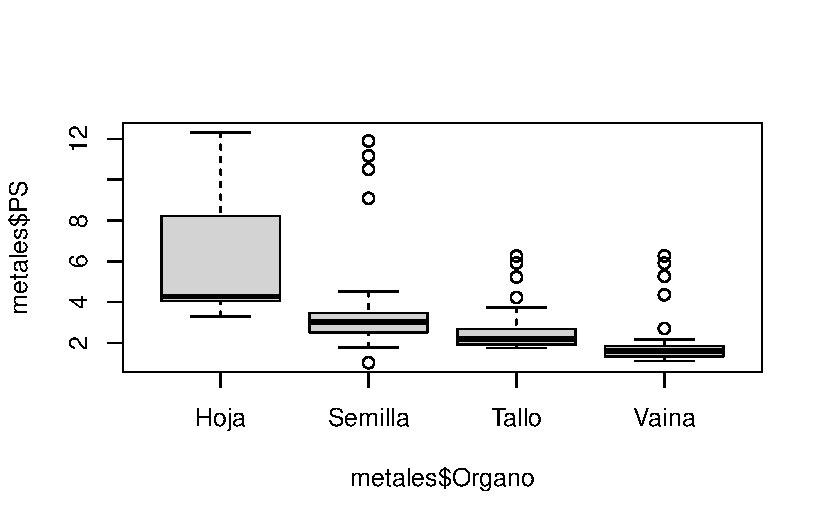
\includegraphics{curso_R_2025_q_files/figure-pdf/unnamed-chunk-12-1.pdf}

}

}

\end{minipage}%
%
\begin{minipage}[t]{0.50\linewidth}

{\centering 

\raisebox{-\height}{

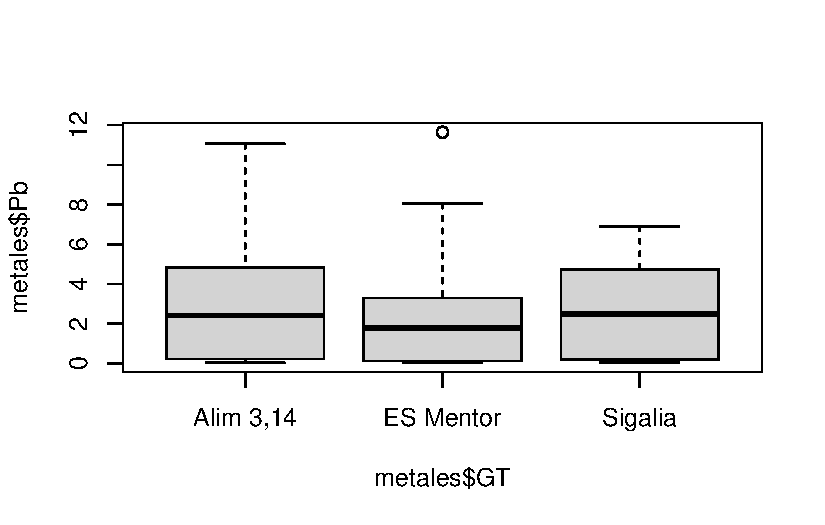
\includegraphics{curso_R_2025_q_files/figure-pdf/unnamed-chunk-12-2.pdf}

}

}

\end{minipage}%
\newline
\begin{minipage}[t]{0.50\linewidth}

{\centering 

\raisebox{-\height}{

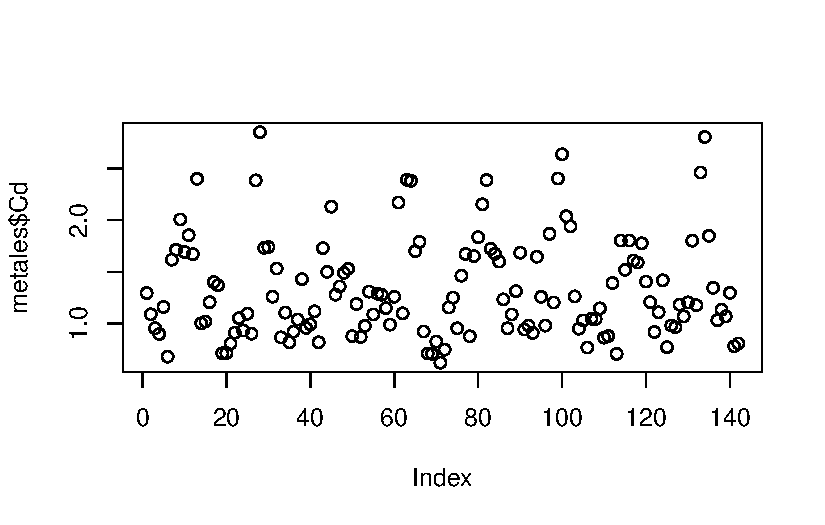
\includegraphics{curso_R_2025_q_files/figure-pdf/unnamed-chunk-12-3.pdf}

}

}

\end{minipage}%
%
\begin{minipage}[t]{0.50\linewidth}

{\centering 

\raisebox{-\height}{

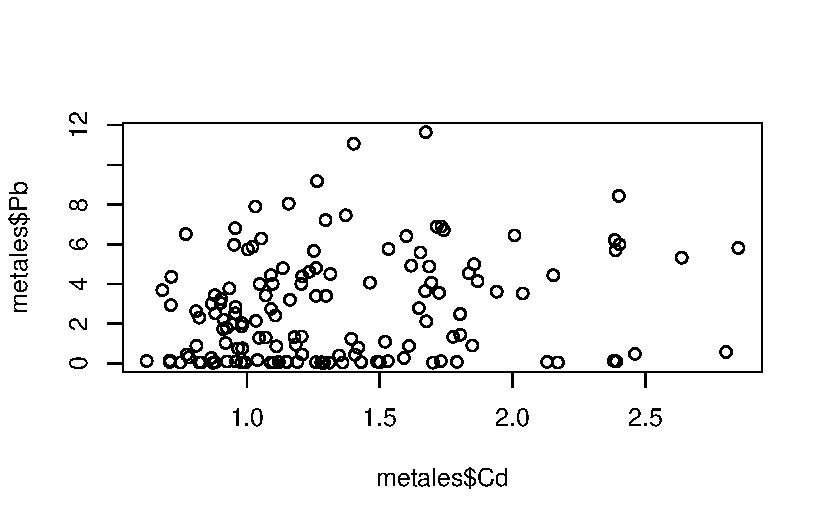
\includegraphics{curso_R_2025_q_files/figure-pdf/unnamed-chunk-12-4.pdf}

}

}

\end{minipage}%

\end{figure}

\hypertarget{manejo-de-la-base-de-datos}{%
\subsection{Manejo de la base de
datos}\label{manejo-de-la-base-de-datos}}

\hypertarget{subdividir-la-base-de-datos}{%
\subsubsection{Subdividir la base de
datos}\label{subdividir-la-base-de-datos}}

Algo muy común en el trabajo en R, es la necesidad de subdividir la base
de datos para utilizar únicamente una parte de ella. Veremos un par de
formas de hacerlo.

Con las funciones que incluye R base, utilizaremos \texttt{subset}. Por
ejemplo para elegir solo las muestras del genotipo \emph{Alim 3,14}:

\begin{Shaded}
\begin{Highlighting}[]
\NormalTok{ALIM }\OtherTok{\textless{}{-}} \FunctionTok{subset}\NormalTok{(metales, metales}\SpecialCharTok{$}\NormalTok{GT}\SpecialCharTok{==}\StringTok{"Alim 3,14"}\NormalTok{)}
\end{Highlighting}
\end{Shaded}

Y creamos un objeto que se llama \emph{ALIM}, nuevamente mediante
\emph{\textless-}.

Otra forma de hacerlo es mediante el uso de pipes (\%\textgreater\%).
Las pipes sirven para concatenar una serie de acciones para modificar
una base de datos. En primer lugar se ubica la base a modificar y entre
cada linea de comando \%\textgreater\% (\emph{Ctrl + Shift + m}). Así,
podemos crear la misma base de antes con \texttt{filter}:

\begin{Shaded}
\begin{Highlighting}[]
\NormalTok{ALIM }\OtherTok{\textless{}{-}}\NormalTok{ metales }\SpecialCharTok{\%\textgreater{}\%} \FunctionTok{filter}\NormalTok{(GT }\SpecialCharTok{==} \StringTok{"Alim 3,14"}\NormalTok{)}
\end{Highlighting}
\end{Shaded}

Si queremos filtrar por más de un parámetro:

\begin{Shaded}
\begin{Highlighting}[]
\CommentTok{\# en dos pasos}
\NormalTok{ALIM\_VyS }\OtherTok{\textless{}{-}}\NormalTok{ metales }\SpecialCharTok{\%\textgreater{}\%}
                    \FunctionTok{filter}\NormalTok{(GT }\SpecialCharTok{==} \StringTok{"Alim 3,14"}\NormalTok{) }\SpecialCharTok{\%\textgreater{}\%} \CommentTok{\# se agrega a lo anterior}
                    \FunctionTok{filter}\NormalTok{(Organo }\SpecialCharTok{==}\StringTok{"Vaina"}\SpecialCharTok{|}\NormalTok{ Organo }\SpecialCharTok{==}\StringTok{"Semilla"}\NormalTok{)}
\end{Highlighting}
\end{Shaded}

\hypertarget{seleccionar-filas-o-columnas}{%
\subsubsection{Seleccionar filas o
columnas}\label{seleccionar-filas-o-columnas}}

En R base, el uso de {[} {]} sirve para seleccionar filas o columnas de
una database, tal que \texttt{data{[}filas,columnas{]}}. En el entorno
de \emph{dplyr} utilizaremos la función \texttt{select} para columnas:

\begin{Shaded}
\begin{Highlighting}[]
\CommentTok{\# seleccionar filas 1 a 3}
\NormalTok{metales[}\DecValTok{1}\SpecialCharTok{:}\DecValTok{3}\NormalTok{,]}
\end{Highlighting}
\end{Shaded}

\begin{verbatim}
# A tibble: 3 x 12
   Pote GT          CO2 ET    Organo    PS    Mn    Cu    Zn    Cd    Pb  SPAD
  <dbl> <chr>     <dbl> <chr> <chr>  <dbl> <dbl> <dbl> <dbl> <dbl> <dbl> <dbl>
1     1 ES Mentor   400 No    Hoja    4.58  53.9 10.3  103.  1.30   7.22  29.5
2     2 ES Mentor   400 No    Hoja    3.61  51.1  7.36 149.  1.09   2.75  21.5
3     3 ES Mentor   400 No    Hoja    4.27  41.7  6.90  96.9 0.956  2.53  24.7
\end{verbatim}

\begin{Shaded}
\begin{Highlighting}[]
\CommentTok{\# seleccionar columnas 1 a 3}
\NormalTok{metales[,}\DecValTok{1}\SpecialCharTok{:}\DecValTok{3}\NormalTok{]}
\end{Highlighting}
\end{Shaded}

\begin{verbatim}
# A tibble: 142 x 3
    Pote GT          CO2
   <dbl> <chr>     <dbl>
 1     1 ES Mentor   400
 2     2 ES Mentor   400
 3     3 ES Mentor   400
 4     4 ES Mentor   400
 5     5 ES Mentor   400
 6     6 ES Mentor   400
 7     7 Sigalia     400
 8     8 Sigalia     400
 9     9 Sigalia     400
10    10 Sigalia     400
# i 132 more rows
\end{verbatim}

\begin{Shaded}
\begin{Highlighting}[]
\NormalTok{metales }\SpecialCharTok{\%\textgreater{}\%} \FunctionTok{select}\NormalTok{(}\DecValTok{1}\SpecialCharTok{:}\DecValTok{3}\NormalTok{)}
\end{Highlighting}
\end{Shaded}

\begin{verbatim}
# A tibble: 142 x 3
    Pote GT          CO2
   <dbl> <chr>     <dbl>
 1     1 ES Mentor   400
 2     2 ES Mentor   400
 3     3 ES Mentor   400
 4     4 ES Mentor   400
 5     5 ES Mentor   400
 6     6 ES Mentor   400
 7     7 Sigalia     400
 8     8 Sigalia     400
 9     9 Sigalia     400
10    10 Sigalia     400
# i 132 more rows
\end{verbatim}

\begin{Shaded}
\begin{Highlighting}[]
\CommentTok{\# seleccionar por nombre de la columna}
\NormalTok{metales }\SpecialCharTok{\%\textgreater{}\%} \FunctionTok{select}\NormalTok{(GT,CO2,Pb)}
\end{Highlighting}
\end{Shaded}

\begin{verbatim}
# A tibble: 142 x 3
   GT          CO2    Pb
   <chr>     <dbl> <dbl>
 1 ES Mentor   400  7.22
 2 ES Mentor   400  2.75
 3 ES Mentor   400  2.53
 4 ES Mentor   400  3.05
 5 ES Mentor   400  3.21
 6 ES Mentor   400  3.69
 7 Sigalia     400  4.93
 8 Sigalia     400  6.89
 9 Sigalia     400  6.45
10 Sigalia     400  4.06
# i 132 more rows
\end{verbatim}

\hypertarget{creaciuxf3n-de-nuevas-variables}{%
\subsubsection{Creación de nuevas
variables}\label{creaciuxf3n-de-nuevas-variables}}

Una opción muy útil ligada al paquete \textbf{dplyr} es la de
transformar nuestras bases de datos para algún gráfico en particular,
sin necesidad de cambiar la tabla original. Para ello utilizaremos la
función \texttt{mutate}, que permite generar muchos cambios en la base
de datos. Por ejemplo, en la base ALIM, si queremos agregar la cantidad
absoluta de Pb extraída:

\begin{Shaded}
\begin{Highlighting}[]
\NormalTok{metales }\OtherTok{\textless{}{-}}\NormalTok{ metales }\SpecialCharTok{\%\textgreater{}\%}
  \FunctionTok{mutate}\NormalTok{(}\StringTok{"Pb\_total"} \OtherTok{=}\NormalTok{ Pb}\SpecialCharTok{*}\NormalTok{PS) }\CommentTok{\# se crea una nueva columna}

\CommentTok{\# para ver la columna nueva}
\NormalTok{metales}\SpecialCharTok{$}\NormalTok{Pb\_total}
\end{Highlighting}
\end{Shaded}

\begin{verbatim}
  [1]  33.06302   9.91306  10.79029  14.08638  15.00876  16.17096  20.29512
  [8]  27.08556  26.89233  16.41048  21.13308  13.07837  90.21291  47.62605
 [15]  34.42750  32.72702 104.37124  60.83160  11.97888  18.05868  11.41854
 [22]   9.45945  26.60670  14.74590  15.39456  10.70520  26.29791  21.00659
 [29]  29.45446  26.90309  56.83056  71.08245  28.40670  20.39830  22.12022
 [36]  15.66058   0.53040   0.21148   0.35308   0.12864   0.18957   0.15876
 [43]   0.34568   0.16218   0.26832   0.16653   0.13771   0.20181   1.30689
 [50]   0.26668   0.24779   0.06052   0.11200   0.13858   0.17000   0.09720
 [57]   0.11232   0.15456   0.21060   0.17806   0.13260   0.18768   0.31376
 [64]   0.43420   0.10500   0.19250   1.15430   1.39783   0.68175   0.09020
 [71]   0.12669   0.09306  19.56636  12.97743  15.53136   8.62628  22.82812
 [78]   6.70020  11.51128   8.49915  10.31240  12.42600   6.58415   3.86750
 [85]  40.15790  17.30625   7.66112  11.69561  13.83342  14.11765   3.68520
 [92]   3.53430   3.21594   5.76495   5.95000   3.79984   8.42044   9.41645
 [99]  11.57807  12.14784   6.73466   7.59570  48.02186  35.38976  33.43392
[106]  22.93984  10.68801   1.87756   0.12788   0.41223   3.65980   1.99801
[113]   0.22490   1.61504   2.01480   4.27158   1.36136   0.36025   8.40807
[120]   1.19240   0.75150   1.33900   1.48086   1.53242   0.71118   0.96642
[127]   0.95130   1.18125   2.77965   2.02789   2.81808   2.32225   0.66102
[134]   1.00975   1.17260   0.57710  12.66513  25.29600  14.93736   7.39102
[141]   0.57288   1.09347
\end{verbatim}

\hypertarget{cambio-en-los-niveles-de-un-factor}{%
\subsubsection{Cambio en los niveles de un
factor}\label{cambio-en-los-niveles-de-un-factor}}

También podemos cambiar los niveles de una factor \texttt{mutate},
mediante la siguiente estructura:

\begin{Shaded}
\begin{Highlighting}[]
\NormalTok{... }\SpecialCharTok{\%\textgreater{}\%}
  \FunctionTok{mutate}\NormalTok{(}\AttributeTok{nombre\_factor =} \FunctionTok{fct\_recode}\NormalTok{(nombre\_factor,}
                        \StringTok{"nombre nuevo"} \OtherTok{=} \StringTok{"nombre viejo"}\NormalTok{))}
\end{Highlighting}
\end{Shaded}

Y podemos incluir una línea para cada nivel que queramos modificar. Por
ejemplo:

\begin{Shaded}
\begin{Highlighting}[]
\NormalTok{ALIM }\SpecialCharTok{\%\textgreater{}\%} \FunctionTok{select}\NormalTok{(CO2, ET, PS) }\SpecialCharTok{\%\textgreater{}\%}
  \FunctionTok{mutate}\NormalTok{(}\AttributeTok{ET =} \FunctionTok{fct\_recode}\NormalTok{(ET,}
                         \StringTok{"Control"}  \OtherTok{=} \StringTok{"No"}\NormalTok{,}
                         \StringTok{"Estrés térmico"} \OtherTok{=} \StringTok{"Si"}\NormalTok{)) }
\end{Highlighting}
\end{Shaded}

\begin{verbatim}
# A tibble: 47 x 3
     CO2 ET                PS
   <dbl> <fct>          <dbl>
 1   400 Control        10.7 
 2   400 Control         8.29
 3   400 Control         5.86
 4   400 Estrés térmico  7.46
 5   400 Estrés térmico  9.43
 6   400 Estrés térmico  8.15
 7   550 Control        11.8 
 8   550 Control        12.3 
 9   550 Control         9.45
10   550 Estrés térmico  8.45
# i 37 more rows
\end{verbatim}

\hypertarget{actividad-1}{%
\subsection{Actividad 1}\label{actividad-1}}

\begin{enumerate}
\def\labelenumi{\arabic{enumi}.}
\tightlist
\item
  Cree a partir de la base de datos original, una que contenga
  únicamente los tallos y hojas del cultivar ES Mentor, y las columnas
  de CO\textsubscript{2}, ET, Organo, PS, Zn y Pb.
\item
  Filtre la base creada para obtener otra que solo tenga aquellos datos
  con más de 3 ppm de Pb.
\end{enumerate}

\href{../}{Volver al inicio}

\hypertarget{unidad-2.-anuxe1lisis-y-representaciuxf3n-de-datos-numuxe9ricos}{%
\section{Unidad 2. Análisis y representación de datos
numéricos}\label{unidad-2.-anuxe1lisis-y-representaciuxf3n-de-datos-numuxe9ricos}}

Veremos los análisis a realizar para procesar variables continuas
(correlación y regresión) y como representarlas gráficamente de una
forma más detallada que como lo vimos hasta ahora.

\hypertarget{correlaciuxf3n}{%
\subsection{Correlación}\label{correlaciuxf3n}}

Cuando queremos evaluar la relación entre 2 variables continuas, sin
establecer relaciones de dependencia, el análisis que debemos hacer es
un análisis de correlación lineal. El test de correlación lineal más
utilizado es el de correlación de Pearson, que nos arroja el coeficiente
de Pearson, que toma valores entre -1 y 1, según la relación sea inversa
o directa. Valores cercanos a cero indican falta de relación entre las
variables. La correlación de Pearson tiene como supuestos la
distribución normal de las variables (entre otros). Debemos poner a
prueba esos supuestos para poder realizar este tipo de análisis.

Comenzaremos creando una base de datos de las semillas:

\begin{Shaded}
\begin{Highlighting}[]
\NormalTok{SEM }\OtherTok{\textless{}{-}}\NormalTok{ metales }\SpecialCharTok{\%\textgreater{}\%} \FunctionTok{filter}\NormalTok{(Organo }\SpecialCharTok{==} \StringTok{"Semilla"}\NormalTok{)}
\end{Highlighting}
\end{Shaded}

Veremos primero como analizar de a pares de variables. Lo recomendable
es iniciar con una exploración gráfica de los datos, en este caso vamos
a relacionar la acumulación de Cu y Zn en semillas.

\begin{Shaded}
\begin{Highlighting}[]
\CommentTok{\# Exploración gráfica}

\FunctionTok{plot}\NormalTok{(SEM}\SpecialCharTok{$}\NormalTok{Cu, }\AttributeTok{pch =} \DecValTok{19}\NormalTok{)}
\FunctionTok{plot}\NormalTok{(SEM}\SpecialCharTok{$}\NormalTok{Zn, }\AttributeTok{pch =} \DecValTok{17}\NormalTok{)}
\FunctionTok{plot}\NormalTok{(SEM}\SpecialCharTok{$}\NormalTok{Cu, SEM}\SpecialCharTok{$}\NormalTok{Zn)}
\end{Highlighting}
\end{Shaded}

\begin{figure}

\begin{minipage}[t]{0.50\linewidth}

{\centering 

\raisebox{-\height}{

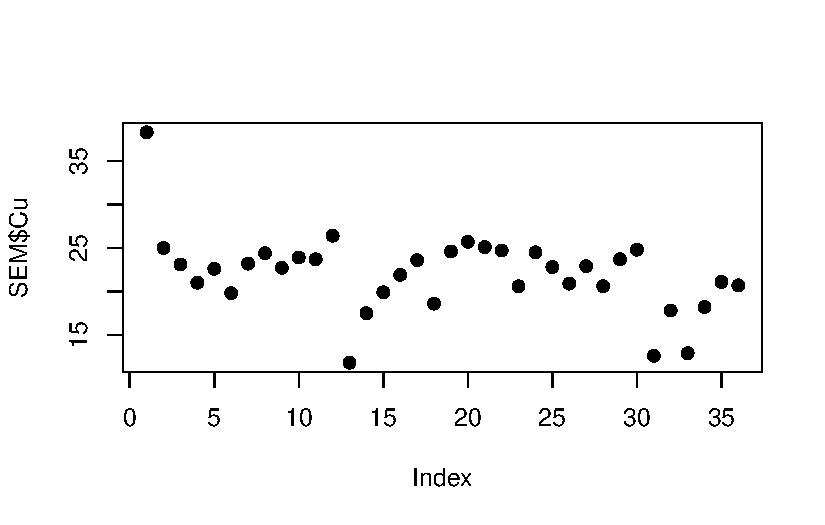
\includegraphics{curso_R_2025_q_files/figure-pdf/unnamed-chunk-21-1.pdf}

}

}

\end{minipage}%
%
\begin{minipage}[t]{0.50\linewidth}

{\centering 

\raisebox{-\height}{

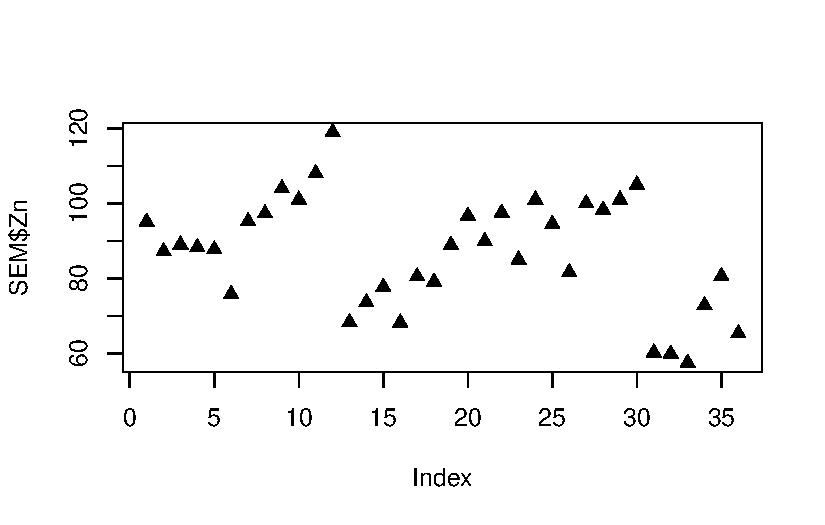
\includegraphics{curso_R_2025_q_files/figure-pdf/unnamed-chunk-21-2.pdf}

}

}

\end{minipage}%
\newline
\begin{minipage}[t]{0.50\linewidth}

{\centering 

\raisebox{-\height}{

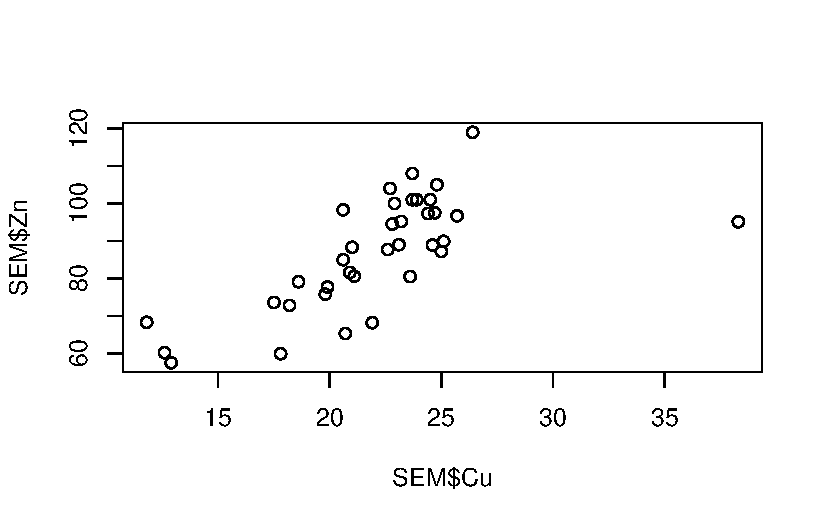
\includegraphics{curso_R_2025_q_files/figure-pdf/unnamed-chunk-21-3.pdf}

}

}

\end{minipage}%

\end{figure}

Vemos que hay un valor extremo en el gráfico de Cu, para identificarlo
podemos correr \emph{identify}:

\begin{Shaded}
\begin{Highlighting}[]
\FunctionTok{plot}\NormalTok{(SEM}\SpecialCharTok{$}\NormalTok{Cu)}
\FunctionTok{identify}\NormalTok{(SEM}\SpecialCharTok{$}\NormalTok{Cu)}
\end{Highlighting}
\end{Shaded}

Ahora veremos cómo hacer la correlación de pearson, de momento ignorando
los supuestos:

\begin{Shaded}
\begin{Highlighting}[]
\FunctionTok{cor.test}\NormalTok{(SEM}\SpecialCharTok{$}\NormalTok{Cu, SEM}\SpecialCharTok{$}\NormalTok{Zn, }\AttributeTok{method =} \StringTok{"pearson"}\NormalTok{)}
\end{Highlighting}
\end{Shaded}

\begin{verbatim}

    Pearson's product-moment correlation

data:  SEM$Cu and SEM$Zn
t = 5.4405, df = 34, p-value = 4.599e-06
alternative hypothesis: true correlation is not equal to 0
95 percent confidence interval:
 0.4558295 0.8256796
sample estimates:
      cor 
0.6822013 
\end{verbatim}

Vemos que nos arroja los resultados del valor del coeficiente lineal de
pearson y su valor p asociado.

\hypertarget{anuxe1lisis-de-normalidad}{%
\subsubsection{Análisis de normalidad}\label{anuxe1lisis-de-normalidad}}

En esta sección veremos cómo poner a prueba la normalidad de nuestros
datos con el test de Shapiro Wilk y como visualizarlo gráficamente en un
qqplot. Recordemos que la hipótesis nula del test es que los datos son
normales, por lo que si rechazamos la hipótesis (p\textless0,05) no hay
normalidad:

\begin{Shaded}
\begin{Highlighting}[]
\CommentTok{\# Forma analítica}

\FunctionTok{shapiro.test}\NormalTok{(SEM}\SpecialCharTok{$}\NormalTok{Cu)}
\FunctionTok{shapiro.test}\NormalTok{(SEM}\SpecialCharTok{$}\NormalTok{Zn)}
\CommentTok{\# Forma gráfica}
\FunctionTok{qqnorm}\NormalTok{(SEM}\SpecialCharTok{$}\NormalTok{Cu)}
\FunctionTok{qqline}\NormalTok{(SEM}\SpecialCharTok{$}\NormalTok{Cu, }\AttributeTok{col=}\StringTok{"red"}\NormalTok{, }\AttributeTok{lwd=}\DecValTok{2}\NormalTok{)}

\FunctionTok{qqnorm}\NormalTok{(SEM}\SpecialCharTok{$}\NormalTok{Zn)}
\FunctionTok{qqline}\NormalTok{(SEM}\SpecialCharTok{$}\NormalTok{Zn, }\AttributeTok{col=}\StringTok{"red"}\NormalTok{, }\AttributeTok{lwd=}\DecValTok{2}\NormalTok{)}
\end{Highlighting}
\end{Shaded}

\begin{figure}

\begin{minipage}[t]{0.50\linewidth}

{\centering 

\begin{verbatim}

    Shapiro-Wilk normality test

data:  SEM$Cu
W = 0.87266, p-value = 0.0006623
\end{verbatim}

}

\end{minipage}%
%
\begin{minipage}[t]{0.50\linewidth}

{\centering 

\begin{verbatim}

    Shapiro-Wilk normality test

data:  SEM$Zn
W = 0.97345, p-value = 0.527
\end{verbatim}

}

\end{minipage}%
\newline
\begin{minipage}[t]{0.50\linewidth}

{\centering 

\raisebox{-\height}{

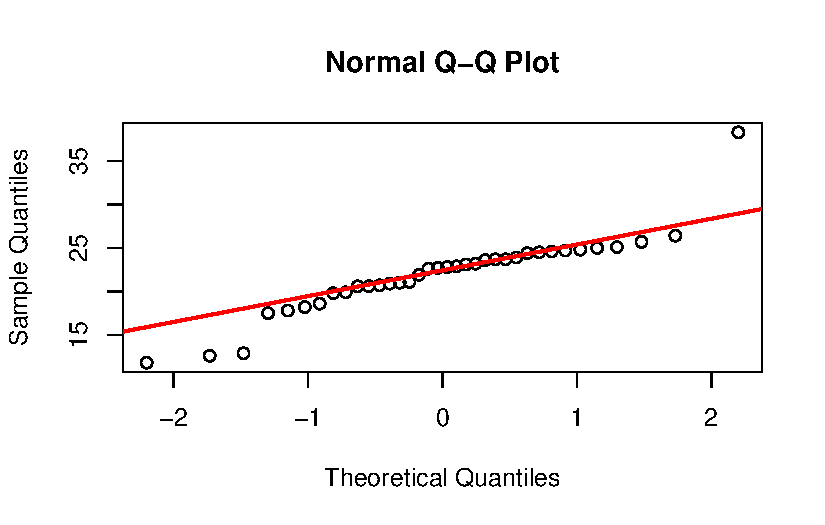
\includegraphics{curso_R_2025_q_files/figure-pdf/unnamed-chunk-24-1.pdf}

}

}

\end{minipage}%
%
\begin{minipage}[t]{0.50\linewidth}

{\centering 

\raisebox{-\height}{

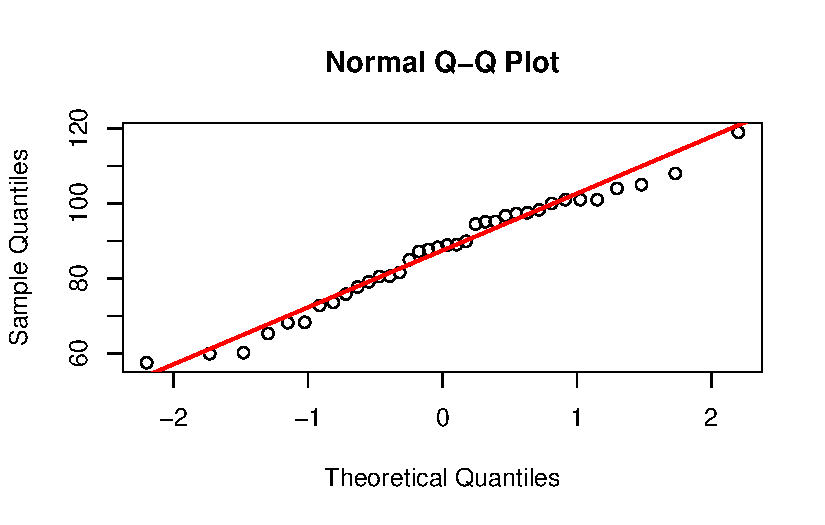
\includegraphics{curso_R_2025_q_files/figure-pdf/unnamed-chunk-24-2.pdf}

}

}

\end{minipage}%

\end{figure}

Vemos que para el caso del Cu no son normales los datos de acuerdo con
el test analítico, aunque el gráfico muestra un valor extremo. En una
primera instancia podemos transformar las variables, que en R lo podemos
hacer directamente:

\begin{Shaded}
\begin{Highlighting}[]
\FunctionTok{shapiro.test}\NormalTok{(}\FunctionTok{log}\NormalTok{(SEM}\SpecialCharTok{$}\NormalTok{Cu)) }\CommentTok{\# convertimos al logaritmo en base 10}
\end{Highlighting}
\end{Shaded}

\begin{verbatim}

    Shapiro-Wilk normality test

data:  log(SEM$Cu)
W = 0.86508, p-value = 0.0004317
\end{verbatim}

\begin{Shaded}
\begin{Highlighting}[]
\FunctionTok{qqnorm}\NormalTok{(}\FunctionTok{log}\NormalTok{(SEM}\SpecialCharTok{$}\NormalTok{Cu))}
\FunctionTok{qqline}\NormalTok{(}\FunctionTok{log}\NormalTok{(SEM}\SpecialCharTok{$}\NormalTok{Cu), }\AttributeTok{col=}\StringTok{"red"}\NormalTok{, }\AttributeTok{lwd=}\DecValTok{2}\NormalTok{)}
\end{Highlighting}
\end{Shaded}

\begin{figure}[H]

{\centering 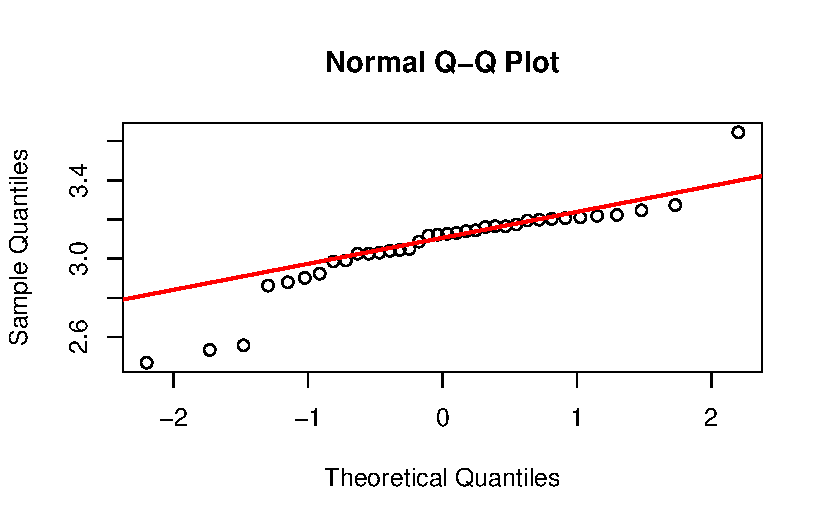
\includegraphics[width=0.5\textwidth,height=\textheight]{curso_R_2025_q_files/figure-pdf/unnamed-chunk-25-1.pdf}

}

\end{figure}

Sigue sin mostrar normalidad. Como vimos antes, el primer valor es mucho
más alto que sus réplicas, si tomáramos la decisión de extraerlo hacemos
el test sin él:

\begin{Shaded}
\begin{Highlighting}[]
\FunctionTok{shapiro.test}\NormalTok{(SEM[}\SpecialCharTok{{-}}\DecValTok{1}\NormalTok{,]}\SpecialCharTok{$}\NormalTok{Cu)}
\end{Highlighting}
\end{Shaded}

\begin{verbatim}

    Shapiro-Wilk normality test

data:  SEM[-1, ]$Cu
W = 0.87851, p-value = 0.001098
\end{verbatim}

\begin{Shaded}
\begin{Highlighting}[]
\FunctionTok{qqnorm}\NormalTok{(SEM[}\SpecialCharTok{{-}}\DecValTok{1}\NormalTok{,]}\SpecialCharTok{$}\NormalTok{Cu)}
\FunctionTok{qqline}\NormalTok{(SEM[}\SpecialCharTok{{-}}\DecValTok{1}\NormalTok{,]}\SpecialCharTok{$}\NormalTok{Cu, }\AttributeTok{col=}\StringTok{"red"}\NormalTok{, }\AttributeTok{lwd=}\DecValTok{2}\NormalTok{)}
\end{Highlighting}
\end{Shaded}

\begin{figure}[H]

{\centering 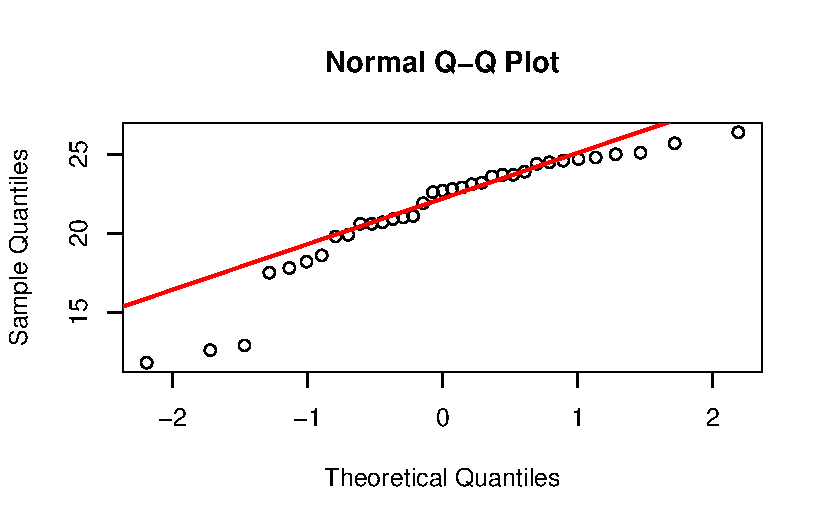
\includegraphics[width=0.5\textwidth,height=\textheight]{curso_R_2025_q_files/figure-pdf/unnamed-chunk-26-1.pdf}

}

\end{figure}

Podemos conformarnos con la eliminación, y correr el test así (no
olvidar eliminar el valor en ambas bases de datos):

\begin{Shaded}
\begin{Highlighting}[]
\FunctionTok{cor.test}\NormalTok{(SEM[}\SpecialCharTok{{-}}\DecValTok{1}\NormalTok{,]}\SpecialCharTok{$}\NormalTok{Cu, SEM[}\SpecialCharTok{{-}}\DecValTok{1}\NormalTok{,]}\SpecialCharTok{$}\NormalTok{Zn, }\AttributeTok{method =} \StringTok{"pearson"}\NormalTok{)}
\end{Highlighting}
\end{Shaded}

\begin{verbatim}

    Pearson's product-moment correlation

data:  SEM[-1, ]$Cu and SEM[-1, ]$Zn
t = 7.5311, df = 33, p-value = 1.161e-08
alternative hypothesis: true correlation is not equal to 0
95 percent confidence interval:
 0.6283377 0.8919974
sample estimates:
      cor 
0.7950977 
\end{verbatim}

Si no logramos de ninguna manera corregir la normalidad, podemos también
correr el test no paramétrico de Spearman que no tiene supuestos
asociados, aunque también presenta menor potencia. En este caso el
coeficiente es el coeficiente de Spearman (\emph{rho}):

\begin{Shaded}
\begin{Highlighting}[]
\FunctionTok{cor.test}\NormalTok{(SEM}\SpecialCharTok{$}\NormalTok{Cu, SEM}\SpecialCharTok{$}\NormalTok{Zn,}
         \AttributeTok{alternative =} \StringTok{"two.sided"}\NormalTok{,}
         \AttributeTok{method =} \StringTok{"spearman"}\NormalTok{, }\AttributeTok{exact =} \ConstantTok{TRUE}\NormalTok{)}
\end{Highlighting}
\end{Shaded}

\begin{verbatim}

    Spearman's rank correlation rho

data:  SEM$Cu and SEM$Zn
S = 2004.8, p-value = 2.233e-07
alternative hypothesis: true rho is not equal to 0
sample estimates:
      rho 
0.7419853 
\end{verbatim}

\hypertarget{muchas-columnas-a-la-vez}{%
\subsubsection{Muchas columnas a la
vez}\label{muchas-columnas-a-la-vez}}

Existen otros test que permiten correlacionar pares de variables pero
correrlas todas a la vez. A diferencia de la función \texttt{cor.test}
que solo admite 2 variables, la función \texttt{cor} permite cargar una
serie de columnas y luego podemos ver los coeficientes en forma
matricial:

\begin{Shaded}
\begin{Highlighting}[]
\NormalTok{CORR }\OtherTok{\textless{}{-}} \FunctionTok{cor}\NormalTok{(SEM[, }\FunctionTok{c}\NormalTok{(}\StringTok{"Pb"}\NormalTok{, }\StringTok{"Cd"}\NormalTok{, }\StringTok{"Mn"}\NormalTok{, }\StringTok{"Cu"}\NormalTok{, }\StringTok{"Zn"}\NormalTok{)],}
            \AttributeTok{use =} \StringTok{"complete.obs"}\NormalTok{, }\AttributeTok{method =} \StringTok{"pearson"}\NormalTok{)}
\NormalTok{CORR }\CommentTok{\# obtenemos los coeficientes}
\end{Highlighting}
\end{Shaded}

\begin{verbatim}
             Pb         Cd         Mn         Cu            Zn
Pb 1.0000000000  0.1480843  0.3825917  0.1104054  0.0009652035
Cd 0.1480843231  1.0000000 -0.3435795  0.2023747  0.6365851679
Mn 0.3825916853 -0.3435795  1.0000000 -0.3945261 -0.3955337272
Cu 0.1104053538  0.2023747 -0.3945261  1.0000000  0.6822013201
Zn 0.0009652035  0.6365852 -0.3955337  0.6822013  1.0000000000
\end{verbatim}

Otra función de utilidad que nos permite ver los coeficientes y los
valores p al mismo tiempo es la función \texttt{rcorr} del paquete
\textbf{Hmisc}:

\begin{Shaded}
\begin{Highlighting}[]
\FunctionTok{library}\NormalTok{(Hmisc)}
\end{Highlighting}
\end{Shaded}

\begin{verbatim}
Warning: package 'Hmisc' was built under R version 4.4.2
\end{verbatim}

\begin{Shaded}
\begin{Highlighting}[]
\NormalTok{CORR.Sem }\OtherTok{\textless{}{-}} \FunctionTok{rcorr}\NormalTok{(}\FunctionTok{as.matrix}\NormalTok{(SEM[,}\DecValTok{7}\SpecialCharTok{:}\DecValTok{11}\NormalTok{])) }\CommentTok{\#argumento matricial}
\NormalTok{CORR.Sem }\CommentTok{\# aquí observamos primero los valores de coeficientes y luego el valor p}
\end{Highlighting}
\end{Shaded}

\begin{verbatim}
      Mn    Cu    Zn    Cd   Pb
Mn  1.00 -0.39 -0.40 -0.34 0.38
Cu -0.39  1.00  0.68  0.20 0.11
Zn -0.40  0.68  1.00  0.64 0.00
Cd -0.34  0.20  0.64  1.00 0.15
Pb  0.38  0.11  0.00  0.15 1.00

n= 36 


P
   Mn     Cu     Zn     Cd     Pb    
Mn        0.0173 0.0170 0.0402 0.0213
Cu 0.0173        0.0000 0.2365 0.5215
Zn 0.0170 0.0000        0.0000 0.9955
Cd 0.0402 0.2365 0.0000        0.3887
Pb 0.0213 0.5215 0.9955 0.3887       
\end{verbatim}

Ahora veremos dos paquetes que nos permiten ver en forma gráfica el
resultado de nuestra correlación. El primero es el paquete
\textbf{corrplot} del cual usaremos las funciones \texttt{cor.mtest} y
\texttt{corrplot}:

\begin{Shaded}
\begin{Highlighting}[]
\FunctionTok{library}\NormalTok{(corrplot)}
\NormalTok{pValues }\OtherTok{\textless{}{-}} \FunctionTok{cor.mtest}\NormalTok{(SEM[,}\DecValTok{7}\SpecialCharTok{:}\DecValTok{11}\NormalTok{]) }\CommentTok{\# generamos un objeto de los valores p}

\FunctionTok{corrplot}\NormalTok{(CORR.Sem}\SpecialCharTok{$}\NormalTok{r,}
         \AttributeTok{type =} \StringTok{"upper"}\NormalTok{,}
         \AttributeTok{tl.col =} \StringTok{"black"}\NormalTok{,}
         \AttributeTok{addCoef.col =} \StringTok{\textquotesingle{}grey20\textquotesingle{}}\NormalTok{,}
         \AttributeTok{p.mat =}\NormalTok{ pValues}\SpecialCharTok{$}\NormalTok{p, }\CommentTok{\# para ver los valores p}
         \AttributeTok{sig.level =} \FloatTok{0.05}\NormalTok{,}
         \AttributeTok{insig =} \StringTok{\textquotesingle{}blank\textquotesingle{}}\NormalTok{,}
         \AttributeTok{tl.srt =} \DecValTok{45}\NormalTok{)}
\end{Highlighting}
\end{Shaded}

\begin{figure}[H]

{\centering 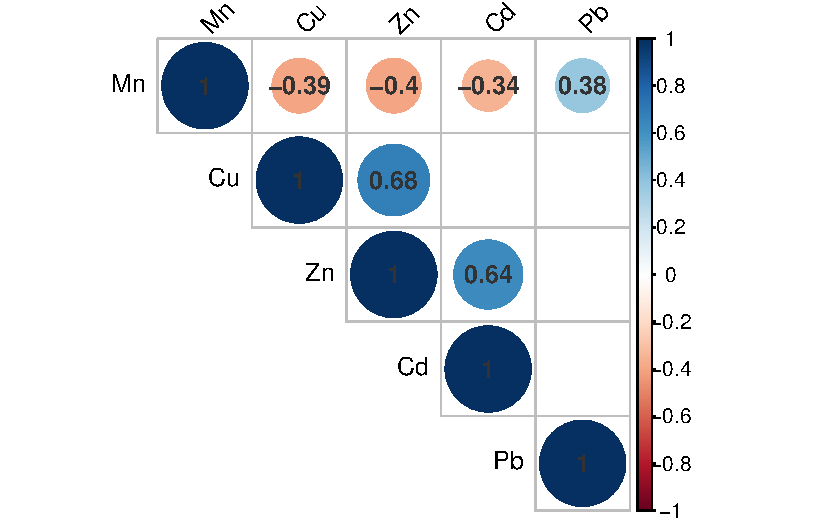
\includegraphics{curso_R_2025_q_files/figure-pdf/unnamed-chunk-31-1.pdf}

}

\end{figure}

Finalmente, introduciré la función \texttt{chart.Correlation} del
paquete \textbf{PerformanceAnalytics}, que permite visualizar
interacciones, gráficos de dispersión, coeficientes de correlación y
significancia todo al mismo tiempo:

\begin{Shaded}
\begin{Highlighting}[]
\FunctionTok{library}\NormalTok{(}\StringTok{"PerformanceAnalytics"}\NormalTok{)}
\FunctionTok{chart.Correlation}\NormalTok{(SEM[,}\DecValTok{9}\SpecialCharTok{:}\DecValTok{11}\NormalTok{],}
                  \AttributeTok{histogram=}\ConstantTok{TRUE}\NormalTok{,}
                  \AttributeTok{method =} \StringTok{"pearson"}\NormalTok{,}
                  \AttributeTok{pch=}\DecValTok{19}\NormalTok{)}
\end{Highlighting}
\end{Shaded}

\begin{figure}[H]

{\centering 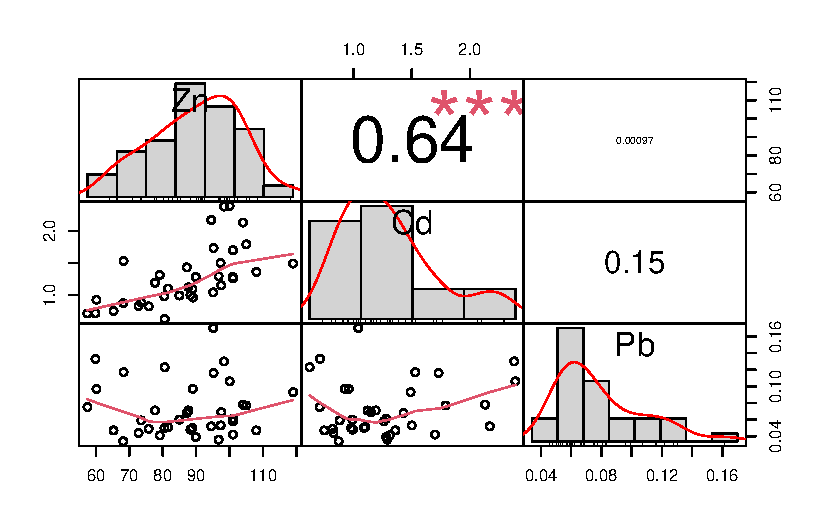
\includegraphics{curso_R_2025_q_files/figure-pdf/unnamed-chunk-32-1.pdf}

}

\end{figure}

Los invito a profundizar más en el uso de los paquetes por su propia
cuenta.

\hypertarget{regresiuxf3n-lineal-simple}{%
\subsection{Regresión lineal simple}\label{regresiuxf3n-lineal-simple}}

El análisis de regresión lineal tiene algunos parecidos con el de
correlación, pero en este caso hay una de la variables que consideramos
que influye en la otra. Es decir, que hay una variable \emph{x}
independiente (regresora) y una \emph{y} dependiente. Ambas variables
deben ser numéricas. El modelo plantea el ajuste lineal de los datos,
por lo tanto hay pruebas de hipótesis para la ordenada al origen y la
pendiente de la recta de ajuste. Los supuestos del modelo son la
distribución normal de las variables y la homogeneidad de los errores.
Un detalle importante, es que el modelo solo es válido en el rango de
nuestra \emph{x}.

Por otro lado, existe un parámetro llamado el coeficiente de
determinación (R\textsuperscript{2}) que nos da una idea de qué
porcentaje de variabilidad de \emph{y} está siendo explicado con
\emph{x}. Este coeficiente toma valores entre 0 y 1, cuanto mayor es
mejor es el ajuste de nuestra nube de puntos a la recta.

En nuestro ejemplo para desarrollar una regresión lineal simple,
relacionaremos el verdor de las hojas (a través de la medición SPAD) con
el Pb acumulado en las mismas. Para ello generaremos una base de datos
para las hojas, y haremos un gráfico rápido para ver esa relación:

\begin{Shaded}
\begin{Highlighting}[]
\NormalTok{HOJA }\OtherTok{\textless{}{-}}\NormalTok{ metales }\SpecialCharTok{\%\textgreater{}\%} \FunctionTok{filter}\NormalTok{(Organo }\SpecialCharTok{==} \StringTok{"Hoja"}\NormalTok{)}

\FunctionTok{plot}\NormalTok{(HOJA}\SpecialCharTok{$}\NormalTok{SPAD, HOJA}\SpecialCharTok{$}\NormalTok{Pb, }\AttributeTok{pch=} \DecValTok{19}\NormalTok{)}
\end{Highlighting}
\end{Shaded}

\begin{figure}[H]

{\centering 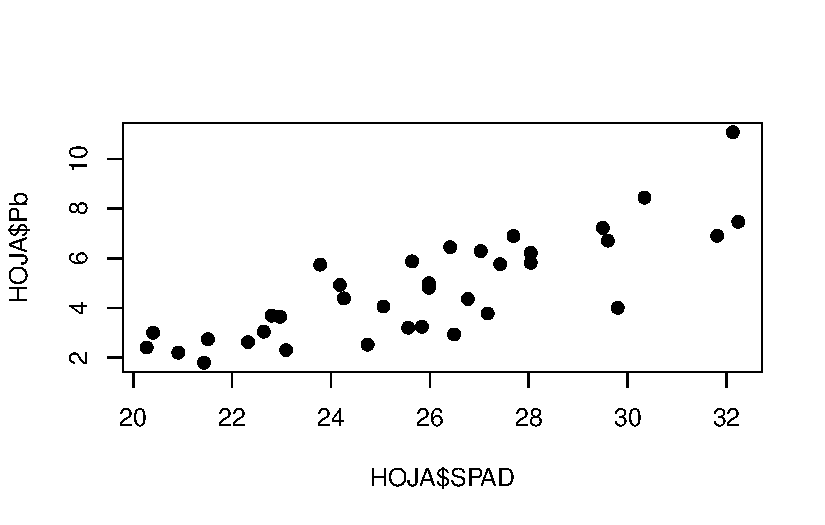
\includegraphics[width=0.6\textwidth,height=\textheight]{curso_R_2025_q_files/figure-pdf/unnamed-chunk-33-1.pdf}

}

\end{figure}

Para realizar una regresión lineal (y que en realidad será de la misma
manera para un ANOVA), se debe plantear un modelo lineal mediante la
función \texttt{lm} de la forma lm(y\textasciitilde x):

\begin{Shaded}
\begin{Highlighting}[]
\NormalTok{fit1 }\OtherTok{\textless{}{-}}\FunctionTok{lm}\NormalTok{(Pb }\SpecialCharTok{\textasciitilde{}}\NormalTok{ SPAD, }\AttributeTok{data =}\NormalTok{ HOJA)}
\end{Highlighting}
\end{Shaded}

Una vez creado el objeto, vamos a poner a prueba los supuestos, tanto de
forma gráfica como analítica. Al someter nuestro modelo a la función
\texttt{plot}, se nos crean 4 gráficos para poner a prueba los
supuestos. Para verlos todos juntos dividiremos la ventana gráfica con
la función \texttt{layout}:

\begin{Shaded}
\begin{Highlighting}[]
\CommentTok{\# Gráfico de supuestos}
\FunctionTok{layout}\NormalTok{(}\FunctionTok{matrix}\NormalTok{(}\DecValTok{1}\SpecialCharTok{:}\DecValTok{4}\NormalTok{, }\DecValTok{2}\NormalTok{, }\DecValTok{2}\NormalTok{)); }\FunctionTok{plot}\NormalTok{(fit1) ;}\FunctionTok{layout}\NormalTok{(}\DecValTok{1}\NormalTok{)}
\end{Highlighting}
\end{Shaded}

\begin{figure}[H]

{\centering 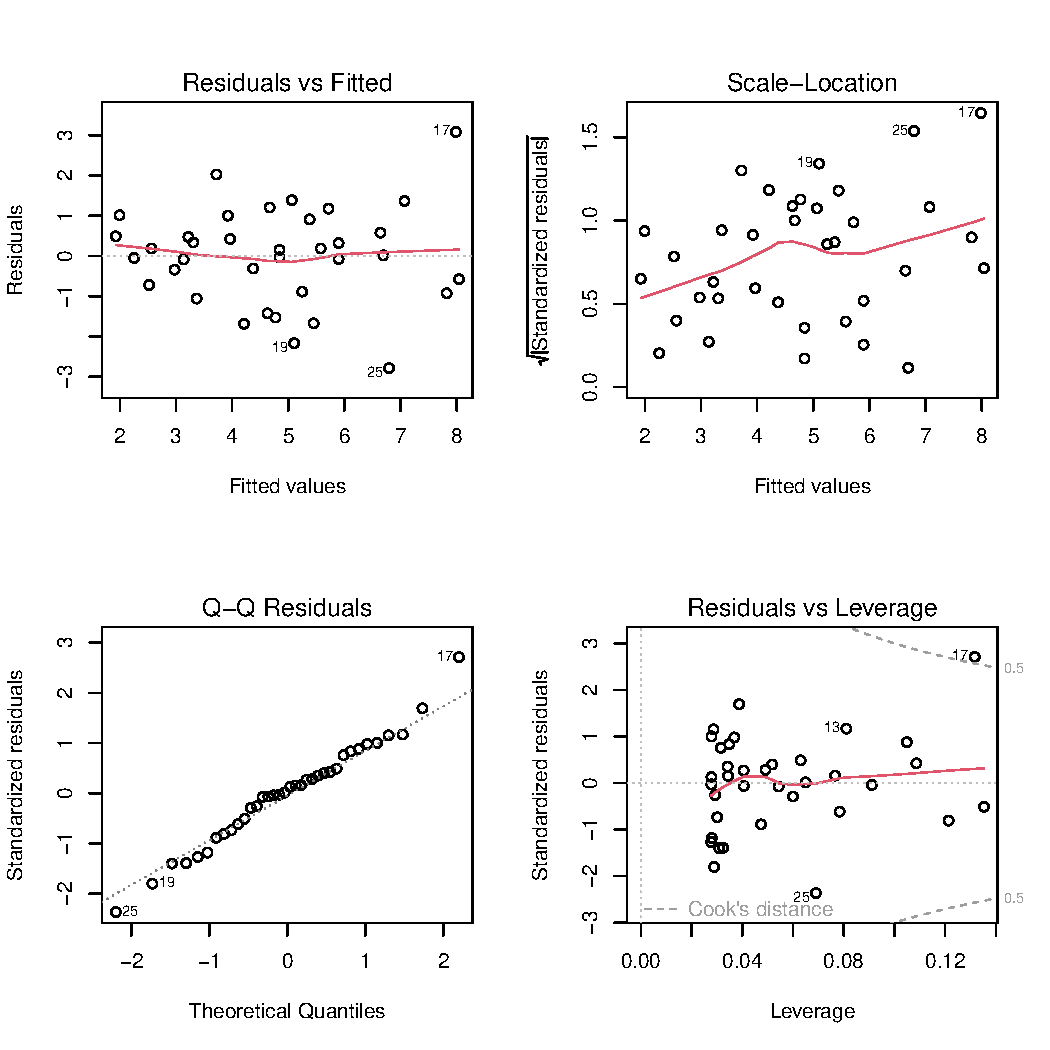
\includegraphics{curso_R_2025_q_files/figure-pdf/unnamed-chunk-35-1.pdf}

}

\end{figure}

Vemos en los dos gráficos superiores la dispersión de los datos, debemos
fijarnos que sea homogénea sin patrones claros. Luego abajo a la derecha
nos aparece en qqplot que ya viéramos anteriormente. Finalmente a la
izquierda el gráfico de \emph{residuos vs leverage} que nos permite
visualizar la distancia de Cook's. En forma resumida este parámetro nos
permite detectar valores muy influyentes en nuestro resultado y que
habría que revisarlos, especialmente si el valor de la distancia es
mayor a 1. En nuestro ejemplo, el valor 17 presenta cierta influencia,
pero no tanta como para concentrarnos en él. Además podemos poner a
prueba de forma analítica la normalidad de los errores:

\begin{Shaded}
\begin{Highlighting}[]
\FunctionTok{shapiro.test}\NormalTok{(}\FunctionTok{resid}\NormalTok{(fit1))}
\end{Highlighting}
\end{Shaded}

\begin{verbatim}

    Shapiro-Wilk normality test

data:  resid(fit1)
W = 0.98603, p-value = 0.9207
\end{verbatim}

Como no se rechaza la hipótesis nula (p\textgreater0,05), no tenemos
evidencia para decir que la distribución no sea normal.

Una vez puestos a prueba los supuestos, procedemos a ver la tabla de
regresión:

\begin{Shaded}
\begin{Highlighting}[]
\FunctionTok{summary}\NormalTok{(fit1)}
\end{Highlighting}
\end{Shaded}

\begin{verbatim}

Call:
lm(formula = Pb ~ SPAD, data = HOJA)

Residuals:
     Min       1Q   Median       3Q      Max 
-2.78646 -0.76173  0.08411  0.66012  3.08197 

Coefficients:
            Estimate Std. Error t value Pr(>|t|)    
(Intercept) -8.43169    1.62522  -5.188 9.79e-06 ***
SPAD         0.51098    0.06243   8.185 1.51e-09 ***
---
Signif. codes:  0 '***' 0.001 '**' 0.01 '*' 0.05 '.' 0.1 ' ' 1

Residual standard error: 1.221 on 34 degrees of freedom
Multiple R-squared:  0.6634,    Adjusted R-squared:  0.6535 
F-statistic:    67 on 1 and 34 DF,  p-value: 1.507e-09
\end{verbatim}

Allí podemos ver los resultados de la prueba de hipótesis para la
ordenada al origen, la pendiente, el valor de R\textsuperscript{2} y el
p del R\textsuperscript{2}. En nuestro caso el modelo obtenido será
\emph{y= -8,43 + 0,51 x} y explica el 65\% de la variabilidad.

El modelo de regresión también puede ser aplicado a una variable
\emph{x} discreta, donde para cada valor de \emph{x} se encuentren
varios valores de \emph{y} . Para ejemplificar vamos a discretizar
nuestra variable SPAD:

\begin{Shaded}
\begin{Highlighting}[]
\CommentTok{\# creamos una nueva columna}
\NormalTok{HOJA}\SpecialCharTok{$}\NormalTok{SPAD\_cat }\OtherTok{\textless{}{-}} \FunctionTok{as.integer}\NormalTok{(}\FunctionTok{round}\NormalTok{(HOJA}\SpecialCharTok{$}\NormalTok{SPAD, }\AttributeTok{digits =} \DecValTok{0}\NormalTok{))}

\FunctionTok{plot}\NormalTok{(HOJA}\SpecialCharTok{$}\NormalTok{SPAD\_cat, HOJA}\SpecialCharTok{$}\NormalTok{Pb, }\AttributeTok{pch=}\DecValTok{19}\NormalTok{)}
\end{Highlighting}
\end{Shaded}

\begin{figure}[H]

{\centering 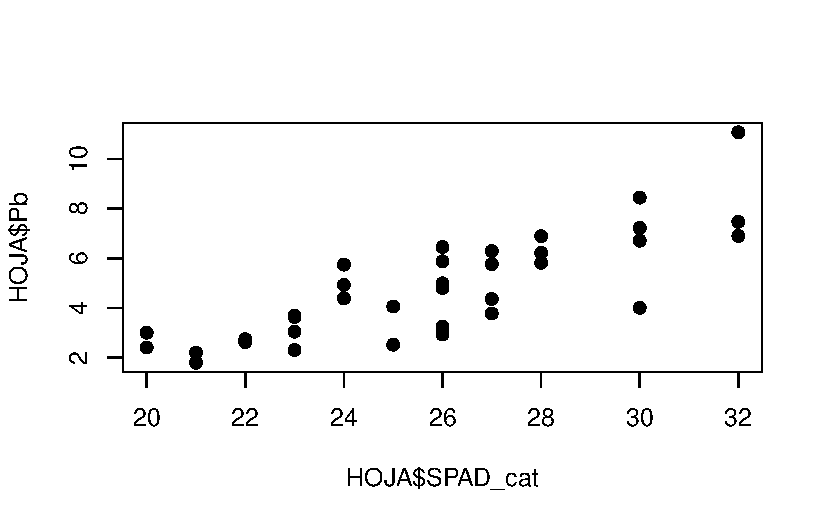
\includegraphics[width=0.75\textwidth,height=\textheight]{curso_R_2025_q_files/figure-pdf/unnamed-chunk-38-1.pdf}

}

\end{figure}

Y corremos nuevamente el modelo, ahora sí podemos hacer un test para
homogeneidad de varianzas y un boxplot de los residuos (errores):

\begin{Shaded}
\begin{Highlighting}[]
\NormalTok{fit2 }\OtherTok{\textless{}{-}}\FunctionTok{lm}\NormalTok{(Pb }\SpecialCharTok{\textasciitilde{}}\NormalTok{ SPAD\_cat, }\AttributeTok{data =}\NormalTok{ HOJA)}

\CommentTok{\# Gráfico de supuestos}
\FunctionTok{layout}\NormalTok{(}\FunctionTok{matrix}\NormalTok{(}\DecValTok{1}\SpecialCharTok{:}\DecValTok{4}\NormalTok{, }\DecValTok{2}\NormalTok{, }\DecValTok{2}\NormalTok{)); }\FunctionTok{plot}\NormalTok{(fit2) ;}\FunctionTok{layout}\NormalTok{(}\DecValTok{1}\NormalTok{)}
\end{Highlighting}
\end{Shaded}

\begin{figure}[H]

{\centering 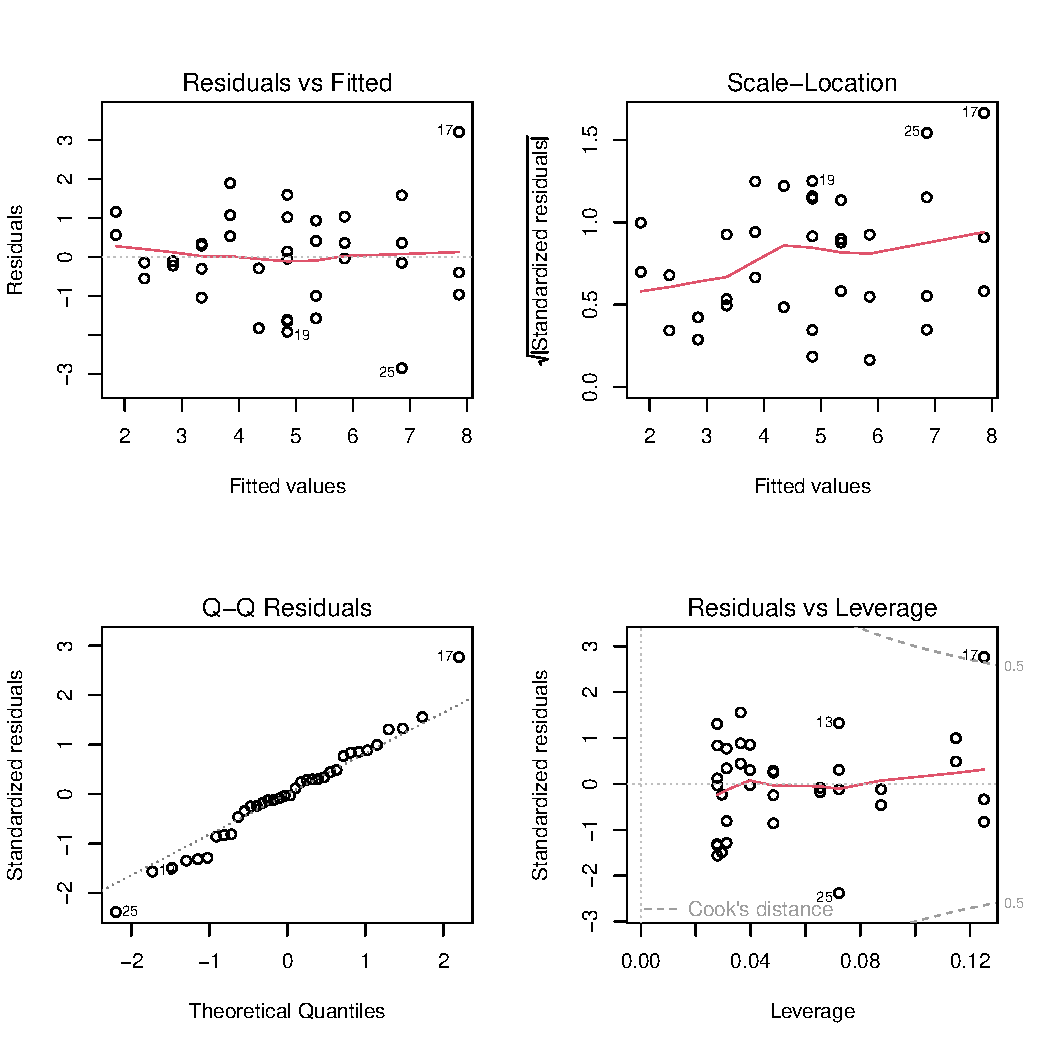
\includegraphics{curso_R_2025_q_files/figure-pdf/unnamed-chunk-39-1.pdf}

}

\end{figure}

\begin{Shaded}
\begin{Highlighting}[]
\FunctionTok{shapiro.test}\NormalTok{(}\FunctionTok{resid}\NormalTok{(fit2))}
\end{Highlighting}
\end{Shaded}

\begin{verbatim}

    Shapiro-Wilk normality test

data:  resid(fit2)
W = 0.98305, p-value = 0.8429
\end{verbatim}

\begin{Shaded}
\begin{Highlighting}[]
\FunctionTok{bartlett.test}\NormalTok{(}\FunctionTok{resid}\NormalTok{(fit2)}\SpecialCharTok{\textasciitilde{}}\NormalTok{HOJA}\SpecialCharTok{$}\NormalTok{SPAD\_cat)}
\end{Highlighting}
\end{Shaded}

\begin{verbatim}

    Bartlett test of homogeneity of variances

data:  resid(fit2) by HOJA$SPAD_cat
Bartlett's K-squared = 13.039, df = 10, p-value = 0.2215
\end{verbatim}

\begin{Shaded}
\begin{Highlighting}[]
\FunctionTok{boxplot}\NormalTok{(}\FunctionTok{residuals}\NormalTok{(fit2,}\AttributeTok{type=}\StringTok{"pearson"}\NormalTok{)}\SpecialCharTok{\textasciitilde{}}\NormalTok{HOJA}\SpecialCharTok{$}\NormalTok{SPAD\_cat,}
        \AttributeTok{ylab=}\StringTok{"Pearson standarized residuals"}\NormalTok{)}
\end{Highlighting}
\end{Shaded}

\begin{figure}[H]

{\centering 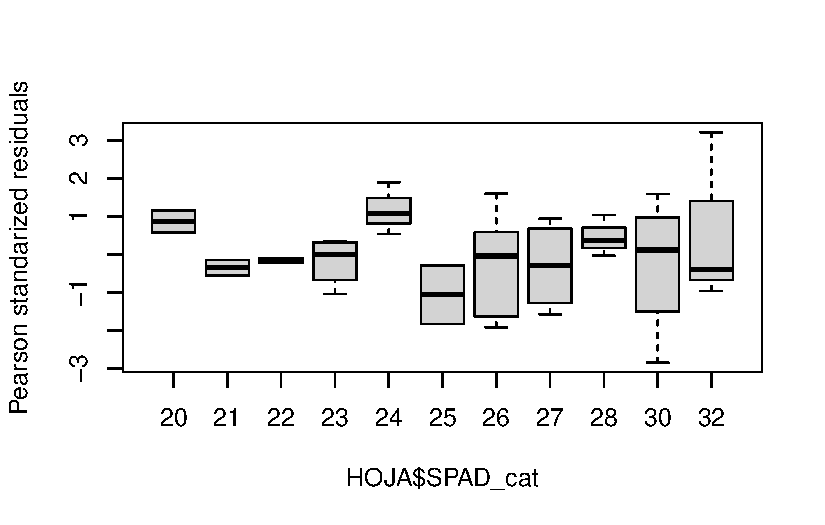
\includegraphics[width=0.75\textwidth,height=\textheight]{curso_R_2025_q_files/figure-pdf/unnamed-chunk-40-1.pdf}

}

\end{figure}

\begin{Shaded}
\begin{Highlighting}[]
\CommentTok{\# Tablas}
\FunctionTok{summary}\NormalTok{(fit2)}
\end{Highlighting}
\end{Shaded}

\begin{verbatim}

Call:
lm(formula = Pb ~ SPAD_cat, data = HOJA)

Residuals:
    Min      1Q  Median      3Q     Max 
-2.8450 -0.6495 -0.0374  0.6626  3.2119 

Coefficients:
            Estimate Std. Error t value Pr(>|t|)    
(Intercept) -8.17737    1.63362  -5.006 1.69e-05 ***
SPAD_cat     0.50105    0.06273   7.988 2.62e-09 ***
---
Signif. codes:  0 '***' 0.001 '**' 0.01 '*' 0.05 '.' 0.1 ' ' 1

Residual standard error: 1.24 on 34 degrees of freedom
Multiple R-squared:  0.6524,    Adjusted R-squared:  0.6421 
F-statistic:  63.8 on 1 and 34 DF,  p-value: 2.623e-09
\end{verbatim}

Vemos que el resultado es muy similar al de antes, por supuesto.

El modelo de regresión lineal puede ser complejizado agregando más
variables regresoras. El planteo del modelo es muy similar, agregando
las nuevas variables y su interacción, por ejemplo para dos regresoras:
lm(y\textasciitilde{} x\textsubscript{1} + x\textsubscript{2} +
x\textsubscript{1}*x\textsubscript{2}). Este tipo de modelos exceden los
alcances de este taller.

\hypertarget{actividad-2}{%
\subsection{Actividad 2}\label{actividad-2}}

\begin{enumerate}
\def\labelenumi{\arabic{enumi}.}
\tightlist
\item
  A partir de la base de datos creada en el punto 1 de la actividad 1,
  realice un modelo de regresión que relaciones el PS con la acumulación
  de Zn en tallos.
\item
  Ponga a prueba los supuestos y concluya.
\end{enumerate}

\begin{center}\rule{0.5\linewidth}{0.5pt}\end{center}

\hypertarget{gruxe1ficos-de-puntos}{%
\subsection{Gráficos de puntos}\label{gruxe1ficos-de-puntos}}

En este apartado veremos cómo una vez que tengamos una correlación o
regresión lineal hecha visualizarla gráficamente de un modo agradable.

\hypertarget{funciuxf3n-plot}{%
\subsubsection{Función plot}\label{funciuxf3n-plot}}

La forma más rápida es mediante la función \texttt{plot} de Rbase

\begin{Shaded}
\begin{Highlighting}[]
\FunctionTok{plot}\NormalTok{(Pb}\SpecialCharTok{\textasciitilde{}}\NormalTok{SPAD, }\AttributeTok{data =}\NormalTok{ HOJA, }\AttributeTok{pch=}\DecValTok{15}\NormalTok{)}
\end{Highlighting}
\end{Shaded}

\begin{figure}[H]

{\centering 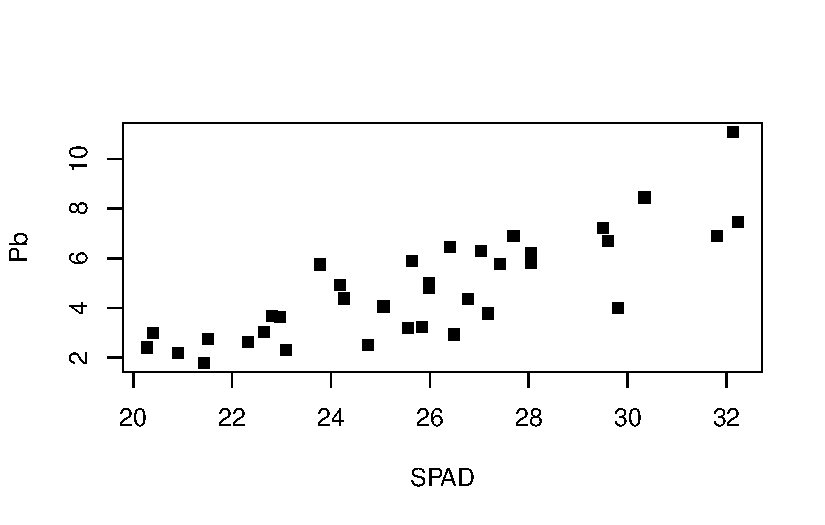
\includegraphics[width=1\textwidth,height=\textheight]{curso_R_2025_q_files/figure-pdf/unnamed-chunk-41-1.pdf}

}

\end{figure}

\hypertarget{funciuxf3n-lineplot.ci-paquete-sciplot}{%
\subsubsection{Función lineplot.CI (paquete
sciplot)}\label{funciuxf3n-lineplot.ci-paquete-sciplot}}

Con el paquete \textbf{sciplot}, podemos crear gráficos de manera rápida
y estéticamente más trabajada con la función \texttt{lineplot.CI}:

\begin{Shaded}
\begin{Highlighting}[]
\FunctionTok{lineplot.CI}\NormalTok{(}\AttributeTok{x.factor =}\NormalTok{ SPAD,}
            \AttributeTok{response =}\NormalTok{ Pb,}
            \AttributeTok{data =}\NormalTok{ HOJA)}
\end{Highlighting}
\end{Shaded}

\begin{figure}[H]

{\centering 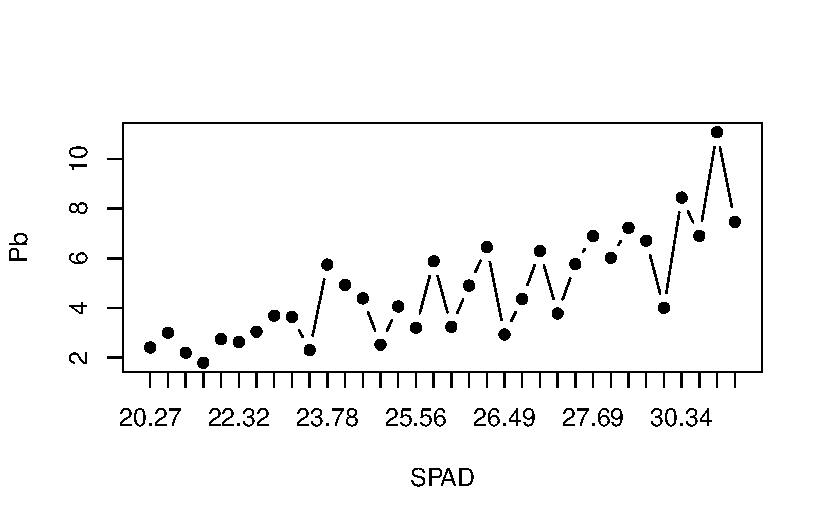
\includegraphics[width=1\textwidth,height=\textheight]{curso_R_2025_q_files/figure-pdf/unnamed-chunk-42-1.pdf}

}

\end{figure}

Si queremos ver qué otras opciones ofrece la función, podemos ir a
buscar la ayuda de la misma. Para ver la ayuda de la función ejecutamos:

\begin{Shaded}
\begin{Highlighting}[]
\NormalTok{?lineplot.CI}
\end{Highlighting}
\end{Shaded}

Y se nos abrirá la ayuda en la ventana 4 de RStudio. Allí vemos una
serie de parámetros que podemos modificar. A su vez podemos subdividir
en grupos, veamos un ejemplo:

\begin{Shaded}
\begin{Highlighting}[]
\FunctionTok{lineplot.CI}\NormalTok{(}\AttributeTok{x.factor =}\NormalTok{ SPAD,}
            \AttributeTok{response =}\NormalTok{ Pb,}
            \AttributeTok{data =}\NormalTok{ HOJA, }\CommentTok{\# dataset}
            \AttributeTok{group =}\NormalTok{ ET, }\CommentTok{\# criterio de agrupamiento}
            \AttributeTok{col=} \FunctionTok{c}\NormalTok{(}\StringTok{"seagreen"}\NormalTok{,}\StringTok{"orange1"}\NormalTok{), }\CommentTok{\# color}
            \AttributeTok{las=}\DecValTok{1}\NormalTok{,  }\CommentTok{\# cambia la inclinación de los números de eje}
            \AttributeTok{ylim =} \FunctionTok{c}\NormalTok{(}\DecValTok{0}\NormalTok{,}\DecValTok{12}\NormalTok{)) }\CommentTok{\# establece los límites del eje y}
\end{Highlighting}
\end{Shaded}

\begin{figure}[H]

{\centering 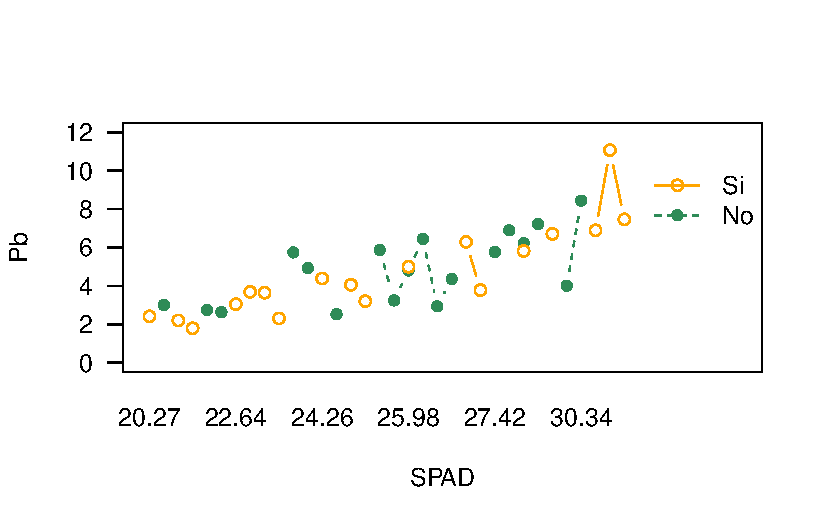
\includegraphics[width=1\textwidth,height=\textheight]{curso_R_2025_q_files/figure-pdf/unnamed-chunk-44-1.pdf}

}

\end{figure}

Todo lo que creamos con la función se denominan parámetros primarios del
gráfico. Luego se le pueden modificar parámetros secundarios como

\begin{Shaded}
\begin{Highlighting}[]
\FunctionTok{lineplot.CI}\NormalTok{(}\AttributeTok{x.factor =}\NormalTok{ SPAD,}
            \AttributeTok{response =}\NormalTok{ Pb,}
            \AttributeTok{data =}\NormalTok{ HOJA,}
            \AttributeTok{ylab =} \StringTok{""}\NormalTok{)}

\CommentTok{\# aquí agregamos los parámetros secundarios}
\FunctionTok{title}\NormalTok{(}\AttributeTok{ylab=} \StringTok{"Pb"}\NormalTok{, }\AttributeTok{line =} \FloatTok{2.5}\NormalTok{) }\CommentTok{\# título del eje eligiendo la distancia}

\FunctionTok{abline}\NormalTok{(}\AttributeTok{h=}\DecValTok{2}\NormalTok{, }\AttributeTok{col=}\StringTok{"red"}\NormalTok{, }\AttributeTok{lty=}\DecValTok{2}\NormalTok{) }\CommentTok{\# línea horizontal}
\FunctionTok{abline}\NormalTok{(}\AttributeTok{v=}\DecValTok{25}\NormalTok{, }\AttributeTok{col=}\StringTok{"red"}\NormalTok{, }\AttributeTok{lty=}\DecValTok{2}\NormalTok{) }\CommentTok{\# línea vertical}
\end{Highlighting}
\end{Shaded}

\begin{figure}[H]

{\centering 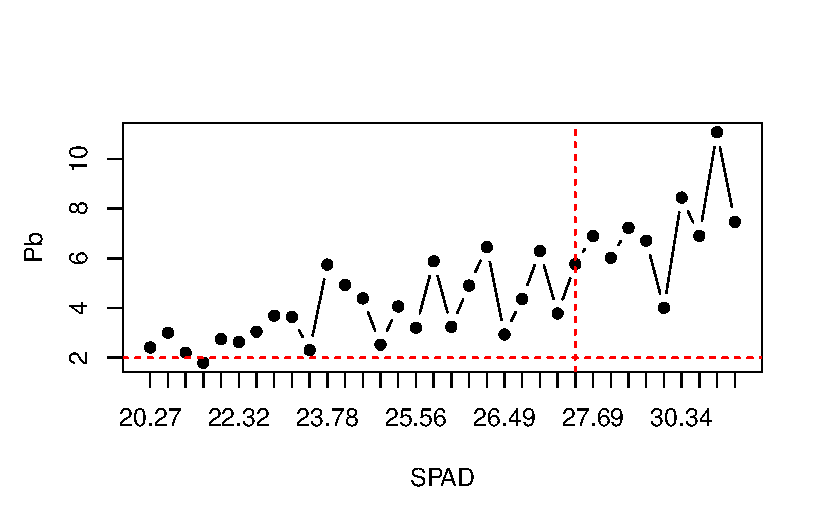
\includegraphics[width=1\textwidth,height=\textheight]{curso_R_2025_q_files/figure-pdf/unnamed-chunk-45-1.pdf}

}

\end{figure}

\hypertarget{funciuxf3n-ggplot-paquete-ggplot2}{%
\subsubsection{Función ggplot (paquete
ggplot2)}\label{funciuxf3n-ggplot-paquete-ggplot2}}

Finalmente introduciremos el paquete gráfico \textbf{ggplot2}. Si bien
es un poco más complicado de aprender y cada gráfico puede requerirnos
más tiempo, es súper versátil y permite hacer infinidad de cosas. La
lógica de trabajo es un poco diferente a las anteriores, ya que aquí se
trabaja en capas que se van separando por el signo +. Todo lo que veamos
en este apartado se aplica a casi cualquier tipo de gráfico con
\texttt{ggplot}, por lo que nos servirá también para variables
categóricas.

\textbf{ggplot2} maneja una composición por capas. En la primera capa
debemos especificar primero la base de datos a utilizar, y luego el
\emph{aesthetic}, es decir, la estructura que tendrán nuestros datos. En
una segunda capa elegiremos el \emph{geom} que dirá la forma que tomará
nuestro gráfico. Con estas capas mínimas podemos obtener un gráfico.

Por ejemplo creamos el gráfico de puntos:

\begin{Shaded}
\begin{Highlighting}[]
\NormalTok{G1 }\OtherTok{\textless{}{-}} \FunctionTok{ggplot}\NormalTok{(}\AttributeTok{data =}\NormalTok{ HOJA, }\CommentTok{\# el data set}
       \FunctionTok{aes}\NormalTok{(}\AttributeTok{x =}\NormalTok{ SPAD, }\AttributeTok{y =}\NormalTok{ Pb)) }\SpecialCharTok{+} \CommentTok{\# x e y dentro de aes}
      \FunctionTok{geom\_point}\NormalTok{() }\CommentTok{\# indica que el gráfico es de puntos}
\NormalTok{G1}
\end{Highlighting}
\end{Shaded}

\begin{figure}[H]

{\centering 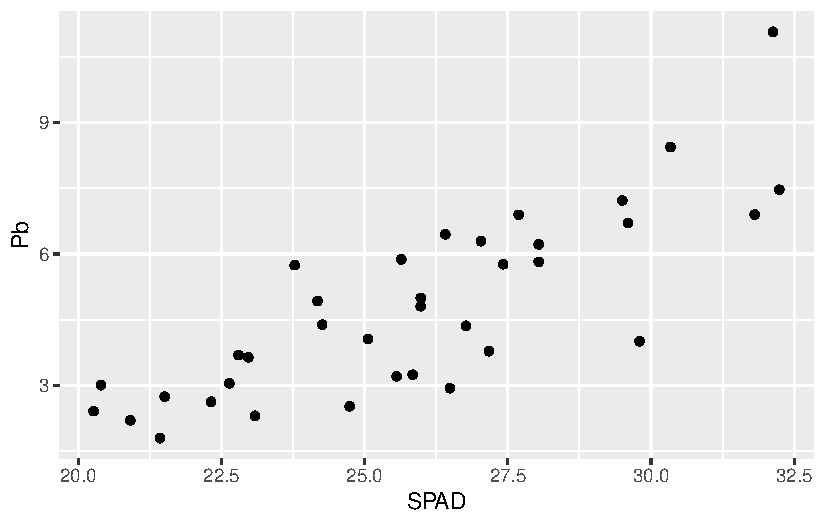
\includegraphics[width=1\textwidth,height=\textheight]{curso_R_2025_q_files/figure-pdf/unnamed-chunk-46-1.pdf}

}

\end{figure}

A partir de acá, podemos ir agregando en sucesivas líneas y separados
por signo + las características que queramos modificar. Por ejemplo,
podemos cambiar el tema general del gráfico (veremos mucho más detalle
más adelante) o modificar el aspecto de los puntos dentro del
\emph{geom}:

\begin{Shaded}
\begin{Highlighting}[]
\FunctionTok{ggplot}\NormalTok{(HOJA, }\FunctionTok{aes}\NormalTok{(SPAD, Pb)) }\SpecialCharTok{+} 
  \FunctionTok{geom\_point}\NormalTok{() }\SpecialCharTok{+} 
  \FunctionTok{theme\_bw}\NormalTok{()}

\FunctionTok{ggplot}\NormalTok{(HOJA, }\FunctionTok{aes}\NormalTok{(SPAD, Pb)) }\SpecialCharTok{+} 
  \FunctionTok{geom\_point}\NormalTok{(}\AttributeTok{size =} \DecValTok{3}\NormalTok{, }\AttributeTok{col =} \StringTok{"yellow"}\NormalTok{) }\SpecialCharTok{+}  \CommentTok{\# cambiamos tamaño y color}
  \FunctionTok{theme\_dark}\NormalTok{()}
\end{Highlighting}
\end{Shaded}

\begin{figure}

\begin{minipage}[t]{0.50\linewidth}

{\centering 

\raisebox{-\height}{

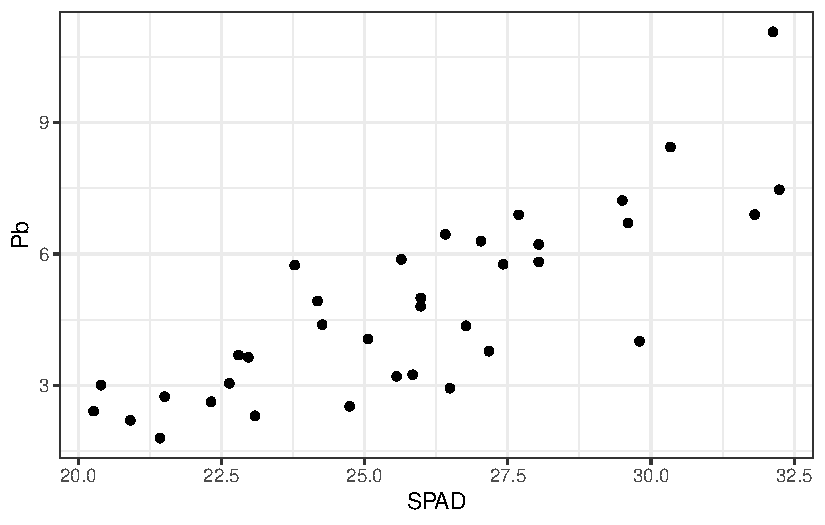
\includegraphics{curso_R_2025_q_files/figure-pdf/unnamed-chunk-47-1.pdf}

}

}

\end{minipage}%
%
\begin{minipage}[t]{0.50\linewidth}

{\centering 

\raisebox{-\height}{

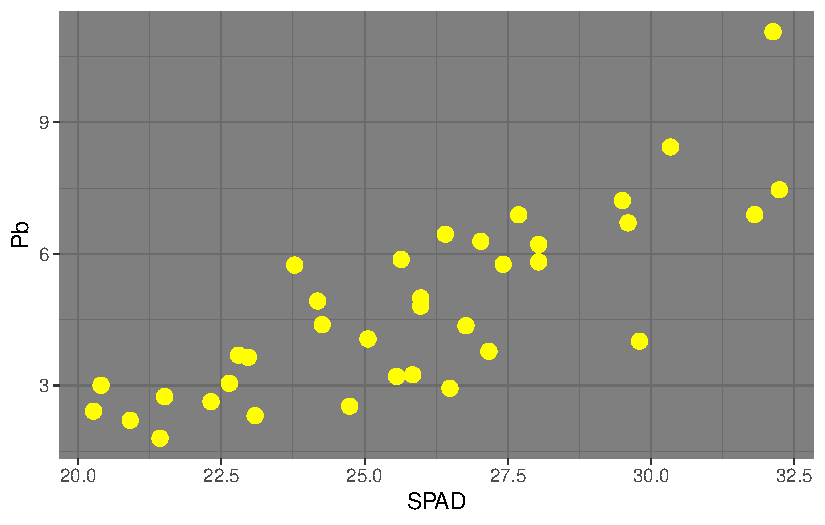
\includegraphics{curso_R_2025_q_files/figure-pdf/unnamed-chunk-47-2.pdf}

}

}

\end{minipage}%

\end{figure}

Podemos agregar nuevas capas con otros \emph{geoms} al mismo gráfico.
Así se puede agregar una línea que una los puntos (con un
\emph{geom\_line}) o una línea de regresión con su intervalo de
confianza (\textbf{geom\_smooth}). Es importante mencionar que el orden
en el que incluyamos las capas afecta al resultado, la última aparecerá
más arriba:

\begin{Shaded}
\begin{Highlighting}[]
\NormalTok{G1 }\SpecialCharTok{+} \FunctionTok{geom\_line}\NormalTok{(}\AttributeTok{col=}\StringTok{"deeppink3"}\NormalTok{) }\CommentTok{\# cambiamos el color en los parámetros del geom}
\NormalTok{G1 }\SpecialCharTok{+} \FunctionTok{geom\_smooth}\NormalTok{(}\AttributeTok{method =} \StringTok{"lm"}\NormalTok{)}
\end{Highlighting}
\end{Shaded}

\begin{verbatim}
`geom_smooth()` using formula = 'y ~ x'
\end{verbatim}

\begin{figure}

\begin{minipage}[t]{0.50\linewidth}

{\centering 

\raisebox{-\height}{

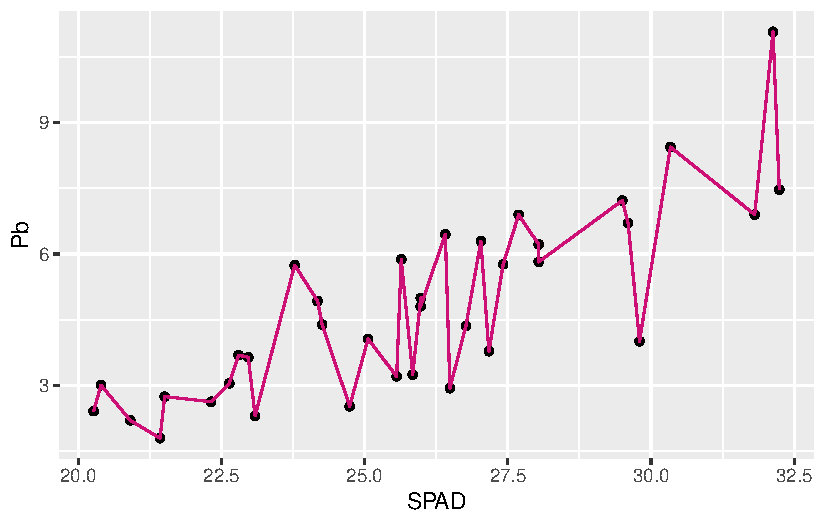
\includegraphics{curso_R_2025_q_files/figure-pdf/unnamed-chunk-48-1.pdf}

}

}

\end{minipage}%
%
\begin{minipage}[t]{0.50\linewidth}

{\centering 

\raisebox{-\height}{

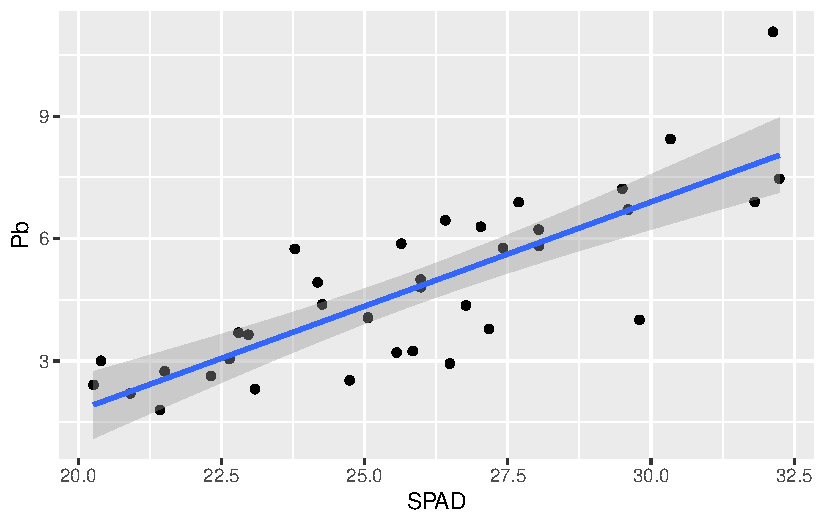
\includegraphics{curso_R_2025_q_files/figure-pdf/unnamed-chunk-48-2.pdf}

}

}

\end{minipage}%

\end{figure}

Al igual que hicimos con \texttt{lineplot.CI}, podemos agrupar los datos
por algún factor según alguna característica que elijamos (color, forma,
relleno, tamaño, etc.). Por ejemplo si queremos distinguir los puntos
por color según el estrés térmico:

\begin{Shaded}
\begin{Highlighting}[]
\NormalTok{G2 }\OtherTok{\textless{}{-}} \FunctionTok{ggplot}\NormalTok{(HOJA,}
             \FunctionTok{aes}\NormalTok{(SPAD, Pb,}
                 \AttributeTok{col =}\NormalTok{ ET)) }\SpecialCharTok{+} \CommentTok{\# agregamos en el aes por qué parámetro dividir}
      \FunctionTok{geom\_point}\NormalTok{()}
\NormalTok{G2}
\end{Highlighting}
\end{Shaded}

\begin{figure}[H]

{\centering 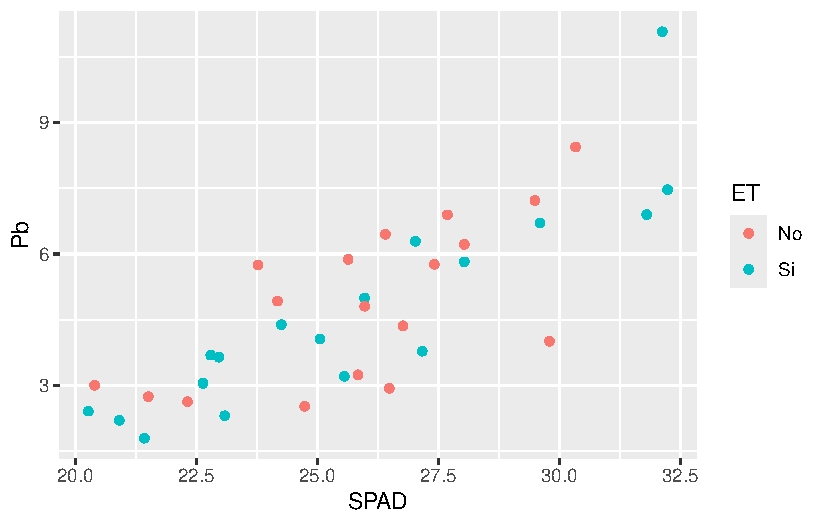
\includegraphics[width=1\textwidth,height=\textheight]{curso_R_2025_q_files/figure-pdf/unnamed-chunk-49-1.pdf}

}

\end{figure}

Ahora si queremos graficar la variable discreta donde para cada valor
del eje \emph{x} tenemos varios valores de \emph{y}, por defecto
\emph{geom\_point} grafica los puntos individualizados, a diferencia de
lo que hacía \emph{lineplot.CI}

\begin{Shaded}
\begin{Highlighting}[]
\FunctionTok{ggplot}\NormalTok{(HOJA, }\FunctionTok{aes}\NormalTok{(SPAD\_cat, Pb)) }\SpecialCharTok{+}
      \FunctionTok{geom\_point}\NormalTok{()}
\end{Highlighting}
\end{Shaded}

\begin{figure}[H]

{\centering 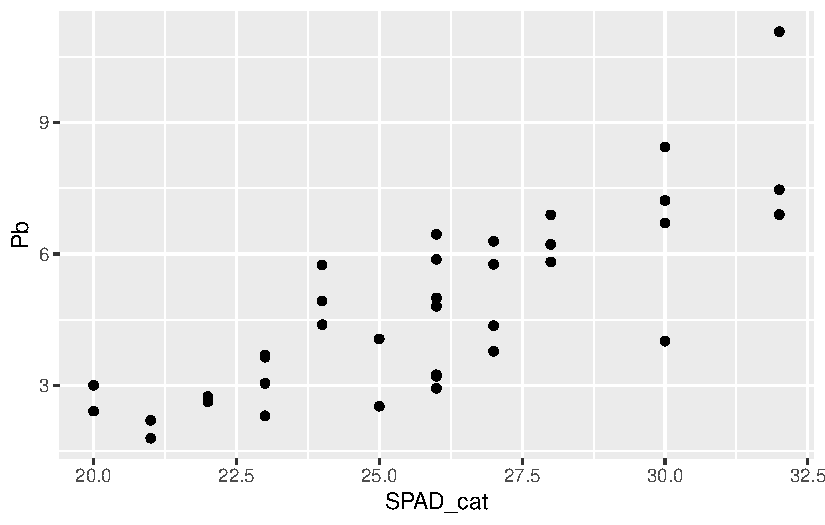
\includegraphics[width=1\textwidth,height=\textheight]{curso_R_2025_q_files/figure-pdf/unnamed-chunk-50-1.pdf}

}

\end{figure}

Entonces para graficar la media y el error estándar, incluimos una capa
de \emph{stat}, que realiza cálculos con la variable respuesta. En este
caso, \textbf{stat\_summary} nos permite graficar el valor medio:

\begin{Shaded}
\begin{Highlighting}[]
\FunctionTok{ggplot}\NormalTok{(}\AttributeTok{data =}\NormalTok{ HOJA,}
       \FunctionTok{aes}\NormalTok{(SPAD\_cat, Pb))}\SpecialCharTok{+}
  \FunctionTok{stat\_summary}\NormalTok{(}\AttributeTok{fun=}\NormalTok{mean, }\AttributeTok{geom=}\StringTok{"point"}\NormalTok{) }\SpecialCharTok{+}
  \FunctionTok{stat\_summary}\NormalTok{(}\AttributeTok{fun.data=}\NormalTok{mean\_se, }\AttributeTok{geom =}\StringTok{\textquotesingle{}errorbar\textquotesingle{}}\NormalTok{)}
\end{Highlighting}
\end{Shaded}

\begin{figure}[H]

{\centering 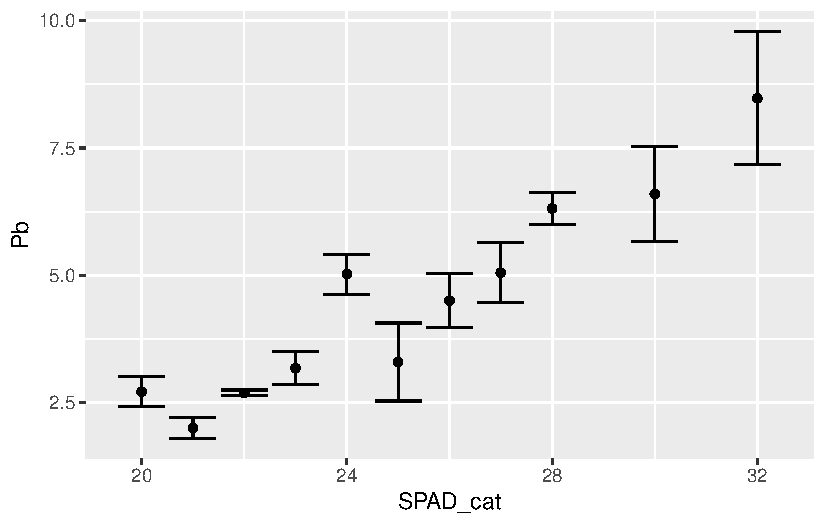
\includegraphics[width=1\textwidth,height=\textheight]{curso_R_2025_q_files/figure-pdf/unnamed-chunk-51-1.pdf}

}

\end{figure}

\begin{Shaded}
\begin{Highlighting}[]
\CommentTok{\# podemos mejorar un poco la estética}
\FunctionTok{ggplot}\NormalTok{(}\AttributeTok{data =}\NormalTok{ HOJA,}
       \FunctionTok{aes}\NormalTok{(SPAD\_cat, Pb))}\SpecialCharTok{+}
  \FunctionTok{stat\_summary}\NormalTok{(}\AttributeTok{fun=}\NormalTok{mean, }\AttributeTok{geom=}\StringTok{"point"}\NormalTok{, }\AttributeTok{size=}\DecValTok{5}\NormalTok{, }\AttributeTok{col =} \StringTok{"azure4"}\NormalTok{) }\SpecialCharTok{+}
  \FunctionTok{stat\_summary}\NormalTok{(}\AttributeTok{fun.data=}\NormalTok{mean\_se, }\AttributeTok{geom =}\StringTok{\textquotesingle{}errorbar\textquotesingle{}}\NormalTok{, }\AttributeTok{width=}\FloatTok{0.2}\NormalTok{)}
\end{Highlighting}
\end{Shaded}

\begin{figure}[H]

{\centering 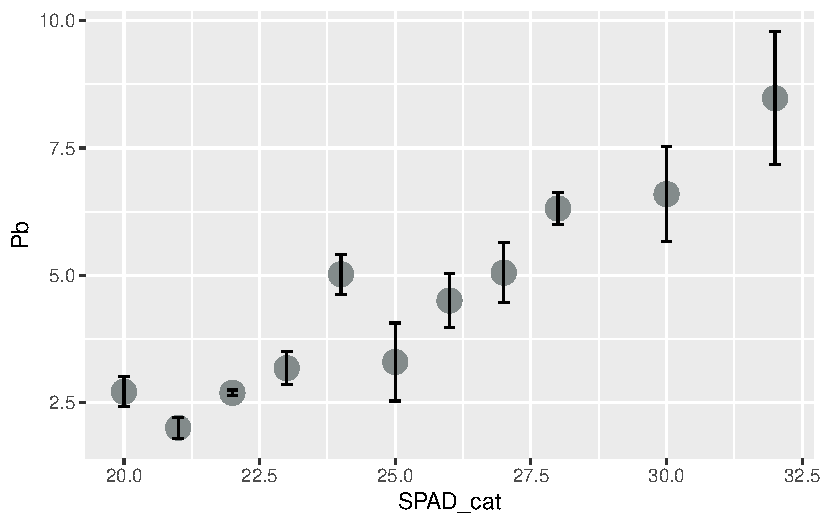
\includegraphics[width=1\textwidth,height=\textheight]{curso_R_2025_q_files/figure-pdf/unnamed-chunk-51-2.pdf}

}

\end{figure}

\hypertarget{actividad-3}{%
\subsubsection{Actividad 3}\label{actividad-3}}

\begin{enumerate}
\def\labelenumi{\arabic{enumi}.}
\tightlist
\item
  Realice una representación gráfica del modelo de regresión realizado
  en la actividad 2. Incorpore en la gráfica una clasificación por
  estrés térmico por color.
\end{enumerate}

\href{../}{Volver al inicio}

\hypertarget{unidad-3.-anuxe1lisis-y-representaciuxf3n-de-datos-categuxf3ricos}{%
\section{Unidad 3. Análisis y representación de datos
categóricos}\label{unidad-3.-anuxe1lisis-y-representaciuxf3n-de-datos-categuxf3ricos}}

\hypertarget{anova-a-1-factor}{%
\subsection{ANOVA a 1 factor}\label{anova-a-1-factor}}

Ahora vamos a trabajar con los datos con variables categóricas. Cuando
incorporamos un factor con diferentes niveles y nos interesa comparar si
hay diferencias entre los efectos de los distintos niveles de uno o más
factores uno de los análisis más utilizados es el análisis de la
varianza. Comenzaremos con el caso de un único factor.

Este análisis plantea la comparación de medias muestrales a partir de la
varianza que presentan los datos dentro de cada grupo (de allí su
nombre). Al igual que el modelo de regresión, presenta supuestos a
cumplirse (normalidad de la variable y homogeneidad de las varianzas).

El planteo del modelo en R será de la misma manera que la regresión, ya
que se trata de otro modelo lineal. En nuestro ejemplo trabajaremos
evaluando el efecto del estrés térmico (inicialmente) en el peso seco de
semillas de la variedad Alim 3,14. Para ello armaremos la base de datos
(doy como ejemplo algunas formas de armarla en base a las que ya
tenemos):

\begin{Shaded}
\begin{Highlighting}[]
\NormalTok{SEM\_Alim }\OtherTok{\textless{}{-}}\NormalTok{ SEM }\SpecialCharTok{\%\textgreater{}\%} \FunctionTok{filter}\NormalTok{(GT }\SpecialCharTok{==} \StringTok{"Alim 3,14"}\NormalTok{)}
\NormalTok{SEM\_Alim }\OtherTok{\textless{}{-}}\NormalTok{ ALIM }\SpecialCharTok{\%\textgreater{}\%} \FunctionTok{filter}\NormalTok{(Organo }\SpecialCharTok{==} \StringTok{"Semilla"}\NormalTok{)}
\NormalTok{SEM\_Alim }\OtherTok{\textless{}{-}}\NormalTok{ ALIM\_VyS }\SpecialCharTok{\%\textgreater{}\%} \FunctionTok{filter}\NormalTok{(Organo }\SpecialCharTok{==} \StringTok{"Semilla"}\NormalTok{)}
\NormalTok{SEM\_Alim }\OtherTok{\textless{}{-}}\NormalTok{ ALIM\_VyS }\SpecialCharTok{\%\textgreater{}\%} \FunctionTok{filter}\NormalTok{(Organo }\SpecialCharTok{!=} \StringTok{"Vaina"}\NormalTok{) }\CommentTok{\# signo diferente a}
\end{Highlighting}
\end{Shaded}

Y ahora sí corremos el modelo y ponemos a prueba los supuestos de igual
manera que hiciéramos anteriormente:

\begin{Shaded}
\begin{Highlighting}[]
\NormalTok{fit3 }\OtherTok{\textless{}{-}}\FunctionTok{lm}\NormalTok{(PS }\SpecialCharTok{\textasciitilde{}}\NormalTok{ ET, }\AttributeTok{data =}\NormalTok{ SEM\_Alim)}

\CommentTok{\# Gráfico de supuestos}
\FunctionTok{layout}\NormalTok{(}\FunctionTok{matrix}\NormalTok{(}\DecValTok{1}\SpecialCharTok{:}\DecValTok{4}\NormalTok{, }\DecValTok{2}\NormalTok{, }\DecValTok{2}\NormalTok{)); }\FunctionTok{plot}\NormalTok{(fit3) ;}\FunctionTok{layout}\NormalTok{(}\DecValTok{1}\NormalTok{)}
\end{Highlighting}
\end{Shaded}

\begin{figure}[H]

{\centering 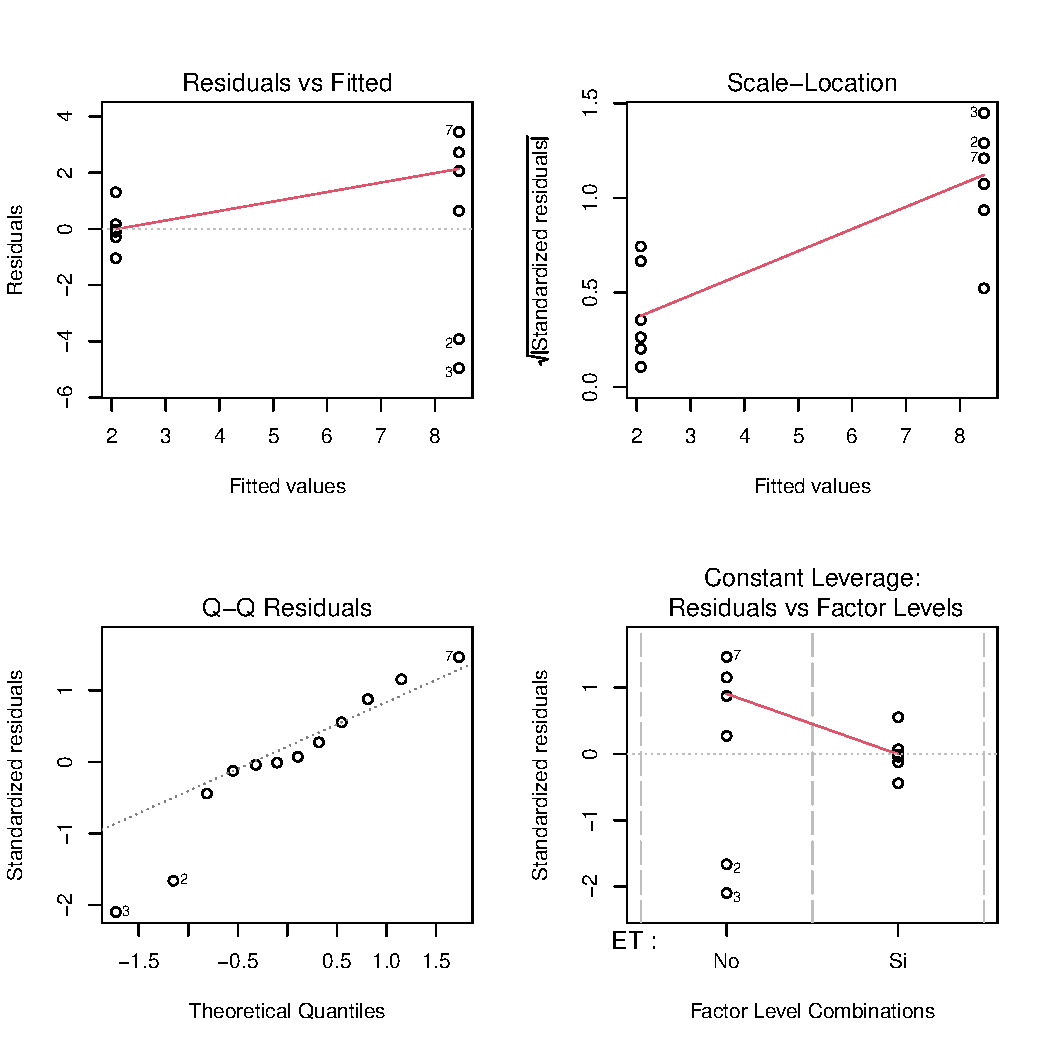
\includegraphics{curso_R_2025_q_files/figure-pdf/unnamed-chunk-53-1.pdf}

}

\end{figure}

\begin{Shaded}
\begin{Highlighting}[]
\FunctionTok{shapiro.test}\NormalTok{(}\FunctionTok{resid}\NormalTok{(fit3))}
\end{Highlighting}
\end{Shaded}

\begin{verbatim}

    Shapiro-Wilk normality test

data:  resid(fit3)
W = 0.92632, p-value = 0.3428
\end{verbatim}

\begin{Shaded}
\begin{Highlighting}[]
\FunctionTok{bartlett.test}\NormalTok{(}\FunctionTok{resid}\NormalTok{(fit3)}\SpecialCharTok{\textasciitilde{}}\NormalTok{SEM\_Alim}\SpecialCharTok{$}\NormalTok{ET) }\CommentTok{\# no hay homogeneidad}
\end{Highlighting}
\end{Shaded}

\begin{verbatim}

    Bartlett test of homogeneity of variances

data:  resid(fit3) by SEM_Alim$ET
Bartlett's K-squared = 8.139, df = 1, p-value = 0.004332
\end{verbatim}

Como vemos hay normalidad de errores pero no homogeneidad de varianza.
Si bien esto pudiera no ser un problema muy grande (el modelo
sobreestimará la varianza general y tendrá menos potencia), podemos
transformar la variable respuesta:

\begin{Shaded}
\begin{Highlighting}[]
\CommentTok{\# Probamos transformando por el logaritmo}
\NormalTok{fit3 }\OtherTok{\textless{}{-}}\FunctionTok{lm}\NormalTok{(}\FunctionTok{log}\NormalTok{(PS) }\SpecialCharTok{\textasciitilde{}}\NormalTok{ ET, }\AttributeTok{data =}\NormalTok{ SEM\_Alim)}

\FunctionTok{layout}\NormalTok{(}\FunctionTok{matrix}\NormalTok{(}\DecValTok{1}\SpecialCharTok{:}\DecValTok{4}\NormalTok{, }\DecValTok{2}\NormalTok{, }\DecValTok{2}\NormalTok{)); }\FunctionTok{plot}\NormalTok{(fit3) ;}\FunctionTok{layout}\NormalTok{(}\DecValTok{1}\NormalTok{)}
\end{Highlighting}
\end{Shaded}

\begin{figure}[H]

{\centering 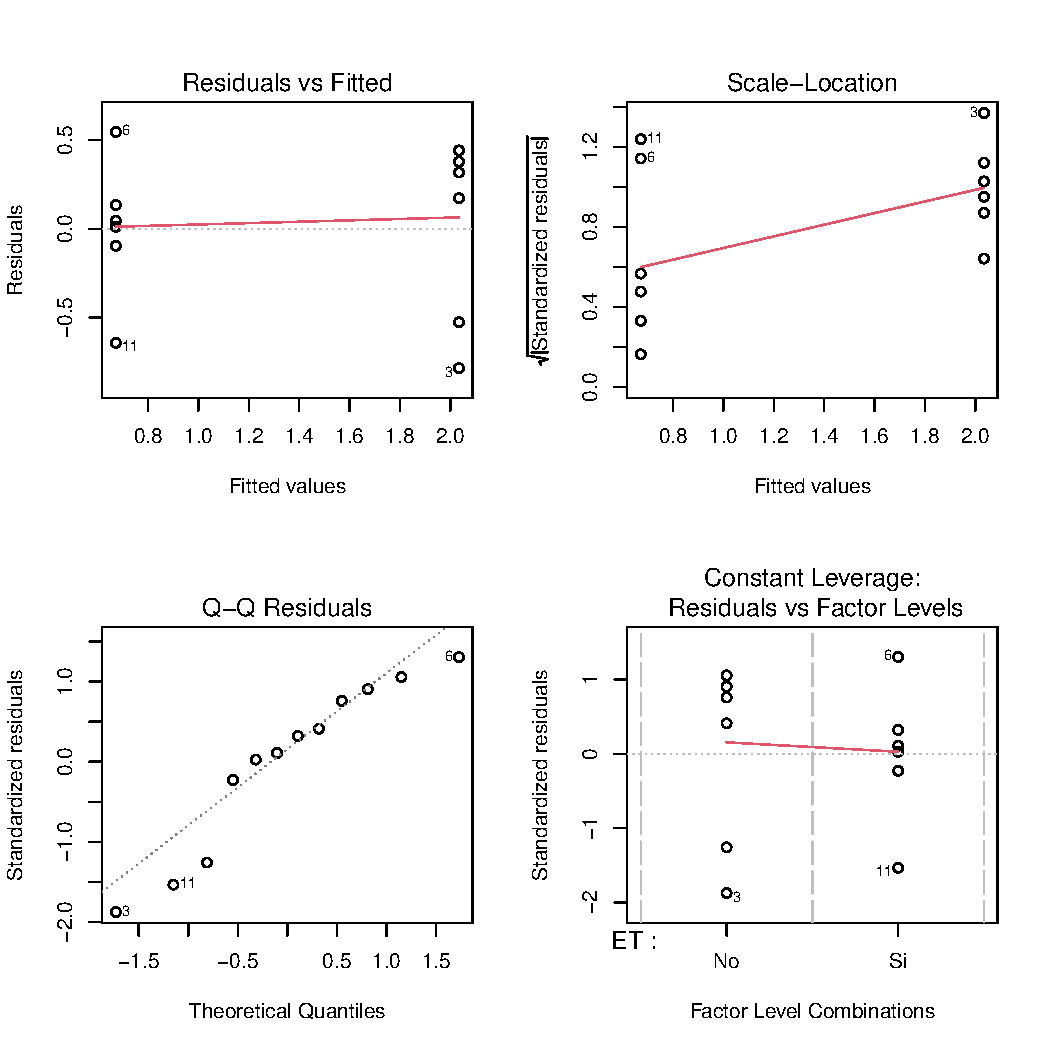
\includegraphics{curso_R_2025_q_files/figure-pdf/unnamed-chunk-54-1.pdf}

}

\end{figure}

\begin{Shaded}
\begin{Highlighting}[]
\FunctionTok{shapiro.test}\NormalTok{(}\FunctionTok{resid}\NormalTok{(fit3))}
\end{Highlighting}
\end{Shaded}

\begin{verbatim}

    Shapiro-Wilk normality test

data:  resid(fit3)
W = 0.91186, p-value = 0.2254
\end{verbatim}

\begin{Shaded}
\begin{Highlighting}[]
\FunctionTok{bartlett.test}\NormalTok{(}\FunctionTok{resid}\NormalTok{(fit3)}\SpecialCharTok{\textasciitilde{}}\NormalTok{SEM\_Alim}\SpecialCharTok{$}\NormalTok{ET)}
\end{Highlighting}
\end{Shaded}

\begin{verbatim}

    Bartlett test of homogeneity of variances

data:  resid(fit3) by SEM_Alim$ET
Bartlett's K-squared = 0.41623, df = 1, p-value = 0.5188
\end{verbatim}

\begin{Shaded}
\begin{Highlighting}[]
\FunctionTok{boxplot}\NormalTok{(}\FunctionTok{residuals}\NormalTok{(fit3,}\AttributeTok{type=}\StringTok{"pearson"}\NormalTok{)}\SpecialCharTok{\textasciitilde{}}\NormalTok{SEM\_Alim}\SpecialCharTok{$}\NormalTok{ET,}
      \AttributeTok{ylab=}\StringTok{"Pearson standarized residuals"}\NormalTok{)}
\end{Highlighting}
\end{Shaded}

\begin{figure}[H]

{\centering 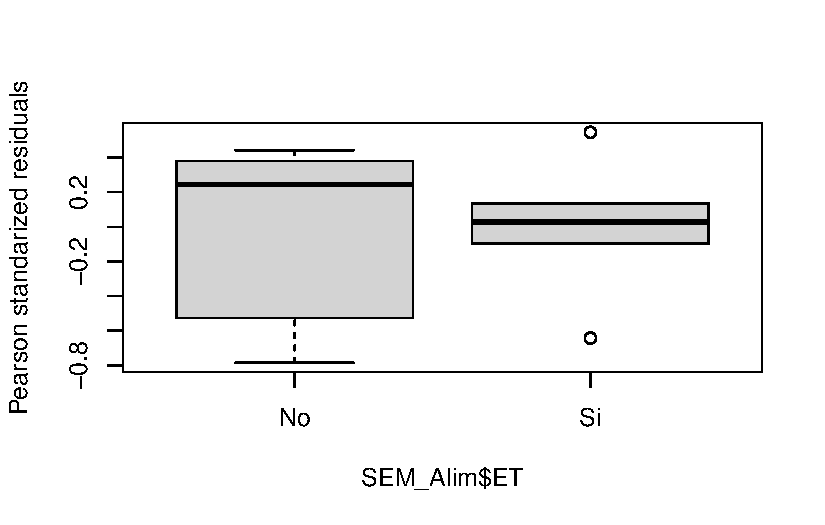
\includegraphics[width=0.5\textwidth,height=\textheight]{curso_R_2025_q_files/figure-pdf/unnamed-chunk-55-1.pdf}

}

\end{figure}

\begin{Shaded}
\begin{Highlighting}[]
\CommentTok{\# ahora sí se cumple}
\end{Highlighting}
\end{Shaded}

Entonces ahora que ya sabemos de la validez del modelo, pediremos la
tabla del ANOVA para ver si existen o no diferencias significativas:

\begin{Shaded}
\begin{Highlighting}[]
\FunctionTok{anova}\NormalTok{(fit3)}
\end{Highlighting}
\end{Shaded}

\begin{verbatim}
Analysis of Variance Table

Response: log(PS)
          Df Sum Sq Mean Sq F value    Pr(>F)    
ET         1 5.5709  5.5709  26.502 0.0004327 ***
Residuals 10 2.1020  0.2102                      
---
Signif. codes:  0 '***' 0.001 '**' 0.01 '*' 0.05 '.' 0.1 ' ' 1
\end{verbatim}

Vemos que arroja un p mucho menor a 0,05, por lo que diremos que al
menos una media es diferente de las otras (como en este caso son dos
niveles, una de la otra). Para saber cuál es diferente de cuál, como
test a posteriori podemos correr el test de Tukey. Para ello utilizamos
la función \texttt{HSD.test} del paquete \textbf{agricolae}:

\begin{Shaded}
\begin{Highlighting}[]
\CommentTok{\# Tukey}
\NormalTok{tukey1 }\OtherTok{\textless{}{-}} \FunctionTok{HSD.test}\NormalTok{(fit3,}\StringTok{"ET"}\NormalTok{)}
\NormalTok{tukey1}\SpecialCharTok{$}\NormalTok{groups}
\end{Highlighting}
\end{Shaded}

\begin{verbatim}
     log(PS) groups
No 2.0346143      a
Si 0.6719101      b
\end{verbatim}

Vemos que sin estrés térmico las semillas tenían mayor peso seco.

\hypertarget{anova-bifactorial}{%
\subsection{ANOVA bifactorial}\label{anova-bifactorial}}

Para correr un modelo de ANOVA con 2 factores diferentes y evaluar su
interacción debemos poner ambas variables separadas por *. Analizaremos
el mismo modelo de antes pero incorporando además el efecto del
CO\textsubscript{2} atmosférico:

\begin{Shaded}
\begin{Highlighting}[]
\NormalTok{SEM\_Alim}\SpecialCharTok{$}\NormalTok{CO2 }\OtherTok{\textless{}{-}} \FunctionTok{as.factor}\NormalTok{(SEM\_Alim}\SpecialCharTok{$}\NormalTok{CO2) }\CommentTok{\# convertimos a factor}
\NormalTok{fit4 }\OtherTok{\textless{}{-}}\FunctionTok{lm}\NormalTok{(PS }\SpecialCharTok{\textasciitilde{}}\NormalTok{ ET}\SpecialCharTok{*}\NormalTok{CO2, }\AttributeTok{data =}\NormalTok{ SEM\_Alim)}
\end{Highlighting}
\end{Shaded}

De la misma manera que antes, probamos los supuestos:

\begin{Shaded}
\begin{Highlighting}[]
\CommentTok{\# Gráfico de supuestos}
\FunctionTok{layout}\NormalTok{(}\FunctionTok{matrix}\NormalTok{(}\DecValTok{1}\SpecialCharTok{:}\DecValTok{4}\NormalTok{, }\DecValTok{2}\NormalTok{, }\DecValTok{2}\NormalTok{)); }\FunctionTok{plot}\NormalTok{(fit4) ;}\FunctionTok{layout}\NormalTok{(}\DecValTok{1}\NormalTok{)}
\end{Highlighting}
\end{Shaded}

\begin{figure}[H]

{\centering 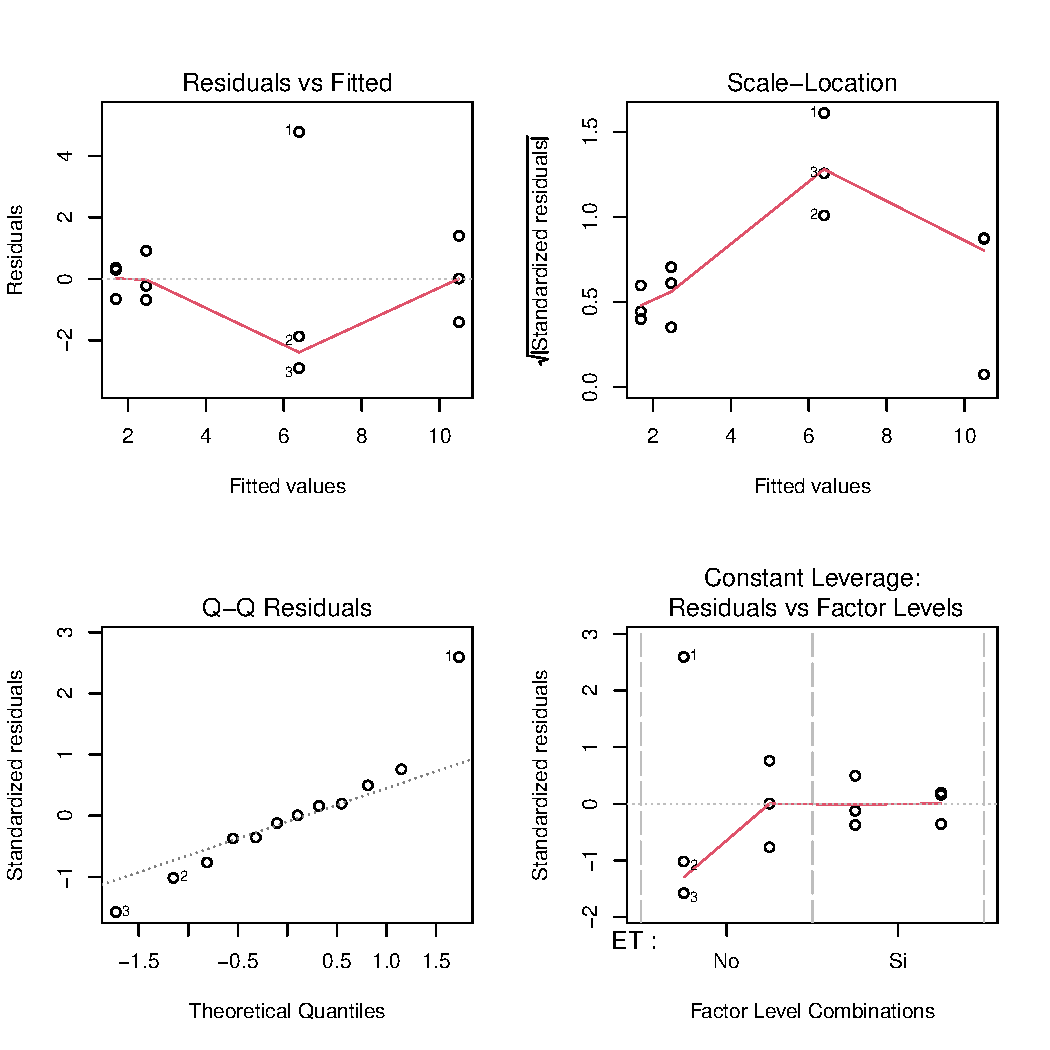
\includegraphics{curso_R_2025_q_files/figure-pdf/unnamed-chunk-59-1.pdf}

}

\end{figure}

\begin{Shaded}
\begin{Highlighting}[]
\CommentTok{\# la homogeneidad se prueba para cada factor}
\FunctionTok{bartlett.test}\NormalTok{(}\FunctionTok{resid}\NormalTok{(fit4)}\SpecialCharTok{\textasciitilde{}}\NormalTok{SEM\_Alim}\SpecialCharTok{$}\NormalTok{ET)}
\FunctionTok{bartlett.test}\NormalTok{(}\FunctionTok{resid}\NormalTok{(fit4)}\SpecialCharTok{\textasciitilde{}}\NormalTok{SEM\_Alim}\SpecialCharTok{$}\NormalTok{CO2)}
\FunctionTok{boxplot}\NormalTok{(}\FunctionTok{residuals}\NormalTok{(fit4,}\AttributeTok{type=}\StringTok{"pearson"}\NormalTok{)}\SpecialCharTok{\textasciitilde{}}\NormalTok{SEM\_Alim}\SpecialCharTok{$}\NormalTok{ET,}
        \AttributeTok{ylab=}\StringTok{"Pearson standarized residuals"}\NormalTok{)}
\FunctionTok{boxplot}\NormalTok{(}\FunctionTok{residuals}\NormalTok{(fit4,}\AttributeTok{type=}\StringTok{"pearson"}\NormalTok{)}\SpecialCharTok{\textasciitilde{}}\NormalTok{SEM\_Alim}\SpecialCharTok{$}\NormalTok{CO2,}
        \AttributeTok{ylab=}\StringTok{"Pearson standarized residuals"}\NormalTok{)}
\end{Highlighting}
\end{Shaded}

\begin{figure}

\begin{minipage}[t]{0.50\linewidth}

{\centering 

\begin{verbatim}

    Bartlett test of homogeneity of variances

data:  resid(fit4) by SEM_Alim$ET
Bartlett's K-squared = 7.6109, df = 1, p-value = 0.005802
\end{verbatim}

}

\end{minipage}%
%
\begin{minipage}[t]{0.50\linewidth}

{\centering 

\begin{verbatim}

    Bartlett test of homogeneity of variances

data:  resid(fit4) by SEM_Alim$CO2
Bartlett's K-squared = 4.1568, df = 1, p-value = 0.04147
\end{verbatim}

}

\end{minipage}%
\newline
\begin{minipage}[t]{0.50\linewidth}

{\centering 

\raisebox{-\height}{

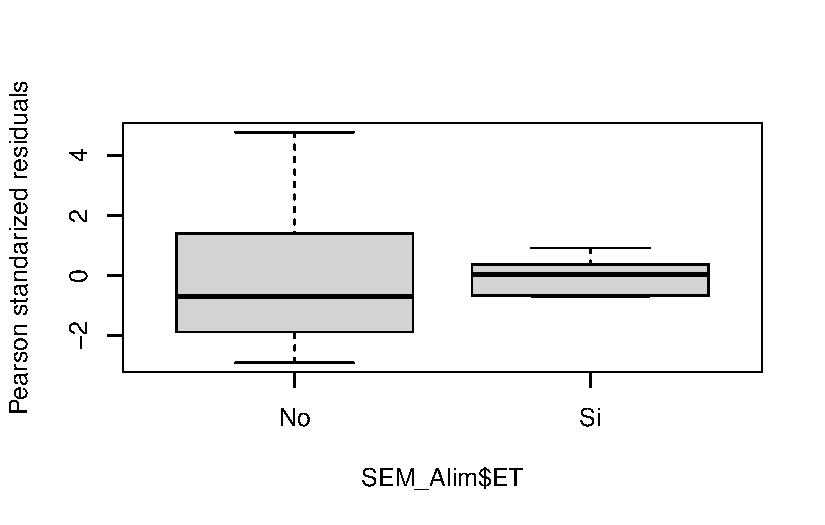
\includegraphics{curso_R_2025_q_files/figure-pdf/unnamed-chunk-60-1.pdf}

}

}

\end{minipage}%
%
\begin{minipage}[t]{0.50\linewidth}

{\centering 

\raisebox{-\height}{

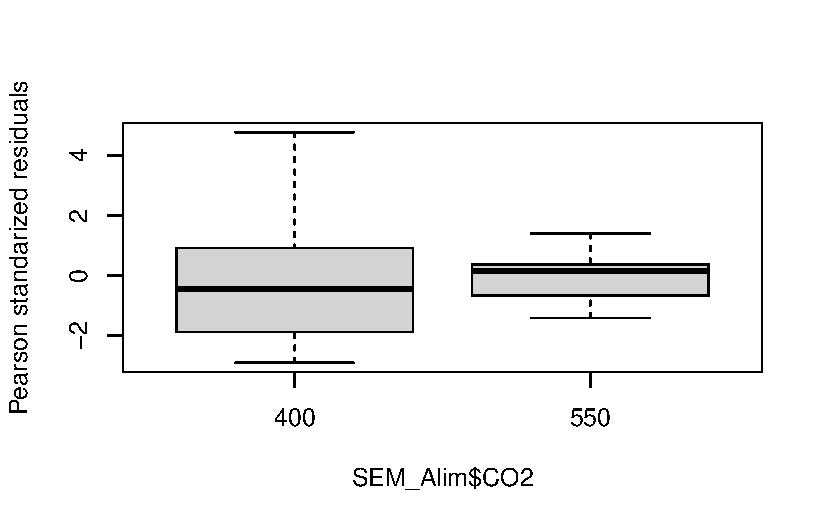
\includegraphics{curso_R_2025_q_files/figure-pdf/unnamed-chunk-60-2.pdf}

}

}

\end{minipage}%

\end{figure}

Una vez comprobados los supuestos, para ver los resultados debemos
ejecutar el comando anova. También podemos ejecutar el summary, que nos
permitirá ver contrastes con respecto al primer nivel del factor:

\begin{Shaded}
\begin{Highlighting}[]
\CommentTok{\# Tablas}
\FunctionTok{anova}\NormalTok{(fit4)}
\end{Highlighting}
\end{Shaded}

\begin{verbatim}
Analysis of Variance Table

Response: PS
          Df Sum Sq Mean Sq F value   Pr(>F)   
ET         1 121.73 121.731 23.9217 0.001207 **
CO2        1   8.30   8.300  1.6311 0.237373   
ET:CO2     1  17.91  17.910  3.5195 0.097500 . 
Residuals  8  40.71   5.089                    
---
Signif. codes:  0 '***' 0.001 '**' 0.01 '*' 0.05 '.' 0.1 ' ' 1
\end{verbatim}

\begin{Shaded}
\begin{Highlighting}[]
\FunctionTok{summary}\NormalTok{(fit4)}
\end{Highlighting}
\end{Shaded}

\begin{verbatim}

Call:
lm(formula = PS ~ ET * CO2, data = SEM_Alim)

Residuals:
    Min      1Q  Median      3Q     Max 
-2.9033 -0.8675 -0.1083  0.5008  4.7767 

Coefficients:
            Estimate Std. Error t value Pr(>|t|)   
(Intercept)    6.393      1.302   4.909  0.00118 **
ETSi          -3.927      1.842  -2.132  0.06560 . 
CO2550         4.107      1.842   2.230  0.05633 . 
ETSi:CO2550   -4.887      2.605  -1.876  0.09750 . 
---
Signif. codes:  0 '***' 0.001 '**' 0.01 '*' 0.05 '.' 0.1 ' ' 1

Residual standard error: 2.256 on 8 degrees of freedom
Multiple R-squared:  0.7842,    Adjusted R-squared:  0.7033 
F-statistic: 9.691 on 3 and 8 DF,  p-value: 0.004853
\end{verbatim}

Vemos que el resultado del ANOVA es significativo únicamente para el
factor ET, por lo que el modelo correcto sería el unifactorial. Sin
embargo mostraremos los test a posteriori para el caso bifactorial:

\begin{Shaded}
\begin{Highlighting}[]
\NormalTok{tukey1 }\OtherTok{\textless{}{-}} \FunctionTok{HSD.test}\NormalTok{(fit4,}\StringTok{"ET"}\NormalTok{)}
\NormalTok{tukey1}\SpecialCharTok{$}\NormalTok{groups}
\end{Highlighting}
\end{Shaded}

\begin{verbatim}
         PS groups
No 8.446667      a
Si 2.076667      b
\end{verbatim}

\begin{Shaded}
\begin{Highlighting}[]
\NormalTok{tukey2 }\OtherTok{\textless{}{-}} \FunctionTok{HSD.test}\NormalTok{(fit4,}\StringTok{"CO2"}\NormalTok{)}
\NormalTok{tukey2}\SpecialCharTok{$}\NormalTok{groups}
\end{Highlighting}
\end{Shaded}

\begin{verbatim}
          PS groups
550 6.093333      a
400 4.430000      a
\end{verbatim}

\begin{Shaded}
\begin{Highlighting}[]
\NormalTok{tukey3 }\OtherTok{\textless{}{-}} \FunctionTok{HSD.test}\NormalTok{(fit4,}\FunctionTok{c}\NormalTok{(}\StringTok{"ET"}\NormalTok{,}\StringTok{"CO2"}\NormalTok{))}
\NormalTok{tukey3}\SpecialCharTok{$}\NormalTok{groups}
\end{Highlighting}
\end{Shaded}

\begin{verbatim}
              PS groups
No:550 10.500000      a
No:400  6.393333     ab
Si:400  2.466667      b
Si:550  1.686667      b
\end{verbatim}

\hypertarget{actividad-4}{%
\subsection{Actividad 4}\label{actividad-4}}

Realice un ANOVA bifactorial con los factores ET y CO2 pero para el peso
seco de semillas de los cultivares ES Mentor y Sigalia. ¿Se observa la
misma respuesta que para el cultivar Alim 3,14?

\hypertarget{gruxe1ficos-de-barras}{%
\subsection{Gráficos de barras}\label{gruxe1ficos-de-barras}}

Nuevamente, veremos varias formas de hacerlos empleando tanto
\textbf{sciplot} como \textbf{ggplot2}.

\hypertarget{bargraph.ci-sciplot}{%
\subsubsection{bargraph.CI (sciplot)}\label{bargraph.ci-sciplot}}

Al igual que para los gráficos de puntos, el paquete \textbf{sciplot}
nos brinda una función para realizar rápidamente un gráfico de barras,
sin necesidad de ejecutar ningún cálculo previo. Por ejemplo:

\begin{Shaded}
\begin{Highlighting}[]
\FunctionTok{bargraph.CI}\NormalTok{(}\AttributeTok{x.factor =}\NormalTok{ ET, }\AttributeTok{response =}\NormalTok{ PS, }\AttributeTok{group =}\NormalTok{ CO2,}
            \AttributeTok{ylim =} \FunctionTok{c}\NormalTok{(}\DecValTok{0}\NormalTok{,}\DecValTok{12}\NormalTok{), }\AttributeTok{legend =}\NormalTok{ T,}
            \AttributeTok{data =}\NormalTok{ SEM\_Alim,  }\AttributeTok{col=} \FunctionTok{c}\NormalTok{(}\StringTok{"honeydew"}\NormalTok{,}\StringTok{"honeydew4"}\NormalTok{),}
            \AttributeTok{las=}\DecValTok{1}\NormalTok{, }\AttributeTok{xlab=}\StringTok{"Estrés térmico"}\NormalTok{,}
            \AttributeTok{ylab=} \StringTok{"Peso seco"}\NormalTok{,}
            \AttributeTok{cex.axis=}\FloatTok{0.8}\NormalTok{);}\FunctionTok{abline}\NormalTok{(}\AttributeTok{h=}\DecValTok{0}\NormalTok{)}
\end{Highlighting}
\end{Shaded}

\begin{figure}[H]

{\centering 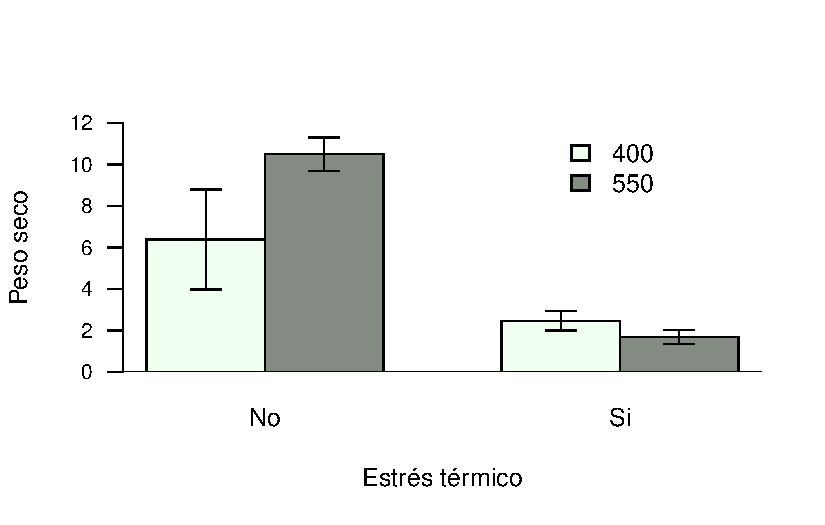
\includegraphics[width=1\textwidth,height=\textheight]{curso_R_2025_q_files/figure-pdf/unnamed-chunk-63-1.pdf}

}

\end{figure}

Los parámetros a modificar son los mismos que vimos anteriormente para
los gráficos de puntos.

\hypertarget{geom_col-ggplot2}{%
\subsubsection{geom\_col (ggplot2)}\label{geom_col-ggplot2}}

\textbf{Ggplot2} nos ofrece dos geoms para hacer gráficos de barras
(\texttt{geom\_col} y \texttt{geom\_bar}). Utilizaremos en este taller
únicamente geom\_col.

Un inconveniente al realizar estos gráficos, es que por defecto el geom
no nos calcula la media y los desvíos de la variable a graficar, sino
que nos representa directamente los datos que le demos. Sin embargo, una
de las principales virtudes de \texttt{ggplot} y del entorno
\textbf{tidyverse} es la posibilidad realizar todos los cambios que
creamos convenientes a nuestro database y luego graficar la base
modificada sin necesidad de haber creado explícitamente un objeto nuevo.
¿Qué ventaja presenta esto? Nos permite manipular fácilmente la base de
datos sin crear una lista muy larga de objetos que luego se nos
complique identificar cuál es cuál. Así, a modo de ejemplo,

Entonces, para realizar el mismo gráfico que hicimos con
\texttt{bargraph.CI}, debemos calcular la media y el error estándar de
la variable PS de semillas:

\begin{Shaded}
\begin{Highlighting}[]
\NormalTok{SEM\_Alim }\SpecialCharTok{\%\textgreater{}\%} \FunctionTok{select}\NormalTok{(CO2, ET, PS) }\SpecialCharTok{\%\textgreater{}\%} \CommentTok{\# seleccionamos las columnas involucradas}
  \FunctionTok{group\_by}\NormalTok{(CO2, ET) }\SpecialCharTok{\%\textgreater{}\%} \CommentTok{\# definimos criterios de agrupamiento}
  \FunctionTok{summarise\_all}\NormalTok{(}\FunctionTok{list}\NormalTok{(mean,se)) }\CommentTok{\# pedimos media y error estándar}
\end{Highlighting}
\end{Shaded}

\begin{verbatim}
# A tibble: 4 x 4
# Groups:   CO2 [2]
  CO2   ET      fn1   fn2
  <fct> <chr> <dbl> <dbl>
1 400   No     6.39 2.41 
2 400   Si     2.47 0.476
3 550   No    10.5  0.811
4 550   Si     1.69 0.329
\end{verbatim}

Vemos que incorpora las columnas \emph{fn1} (que tiene los valores de
las medias) y \emph{fn2} (con los errores estándares). A estos comandos
creados se les anexa el gráfico:

\begin{Shaded}
\begin{Highlighting}[]
\NormalTok{SEM\_Alim }\SpecialCharTok{\%\textgreater{}\%} \FunctionTok{select}\NormalTok{(CO2, ET, PS) }\SpecialCharTok{\%\textgreater{}\%}
  \FunctionTok{group\_by}\NormalTok{(CO2, ET) }\SpecialCharTok{\%\textgreater{}\%}
  \FunctionTok{summarise\_all}\NormalTok{(}\FunctionTok{list}\NormalTok{(mean,se)) }\SpecialCharTok{\%\textgreater{}\%}
  \FunctionTok{ggplot}\NormalTok{(}\FunctionTok{aes}\NormalTok{(ET, fn1, }
             \AttributeTok{fill=}\NormalTok{CO2))}\SpecialCharTok{+} \CommentTok{\# en este caso el parámetro de color lo define fill}
  \FunctionTok{geom\_col}\NormalTok{()}
\end{Highlighting}
\end{Shaded}

\begin{figure}[H]

{\centering 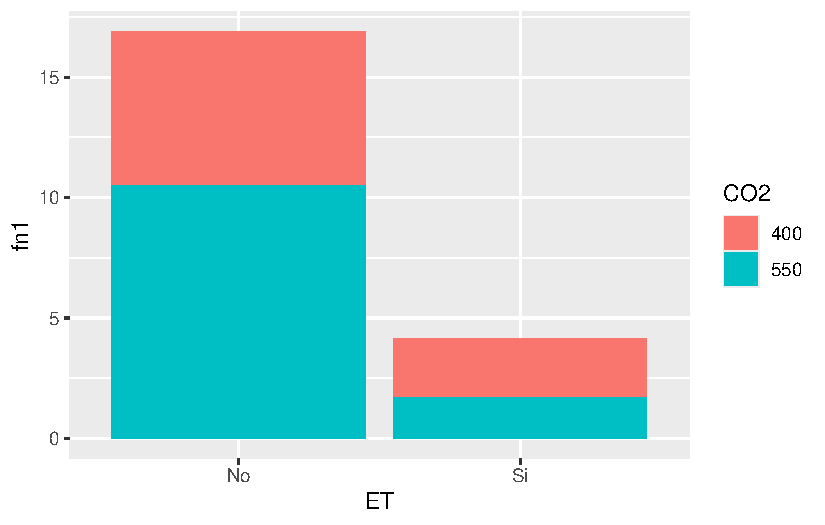
\includegraphics[width=1\textwidth,height=\textheight]{curso_R_2025_q_files/figure-pdf/unnamed-chunk-65-1.pdf}

}

\end{figure}

Como vemos, la barras se apilan. Para que vaya una al lado de la otra,
debemos cambiar el parámetro \emph{position= ``dodge''} dentro del geom
(por defecto está en \emph{identity}). Además agregaremos las barras de
error:

\begin{Shaded}
\begin{Highlighting}[]
\NormalTok{G3 }\OtherTok{\textless{}{-}}\NormalTok{ SEM\_Alim }\SpecialCharTok{\%\textgreater{}\%} \FunctionTok{select}\NormalTok{(CO2, ET, PS) }\SpecialCharTok{\%\textgreater{}\%}
  \FunctionTok{group\_by}\NormalTok{(CO2, ET) }\SpecialCharTok{\%\textgreater{}\%}
  \FunctionTok{summarise\_all}\NormalTok{(}\FunctionTok{list}\NormalTok{(mean,se)) }\SpecialCharTok{\%\textgreater{}\%}
  \FunctionTok{ggplot}\NormalTok{(}\FunctionTok{aes}\NormalTok{(ET, fn1, }\AttributeTok{fill=}\NormalTok{CO2))}\SpecialCharTok{+}
  \FunctionTok{geom\_col}\NormalTok{(}\AttributeTok{position =} \StringTok{"dodge"}\NormalTok{) }\SpecialCharTok{+}
  \FunctionTok{geom\_errorbar}\NormalTok{(}\FunctionTok{aes}\NormalTok{(}\AttributeTok{ymin=}\NormalTok{fn1}\SpecialCharTok{{-}}\NormalTok{fn2, }\AttributeTok{ymax=}\NormalTok{fn1}\SpecialCharTok{+}\NormalTok{fn2), }\AttributeTok{width=}\NormalTok{.}\DecValTok{1}\NormalTok{,}
                \AttributeTok{position =} \FunctionTok{position\_dodge}\NormalTok{(.}\DecValTok{9}\NormalTok{))}
\NormalTok{G3}
\end{Highlighting}
\end{Shaded}

\begin{figure}[H]

{\centering 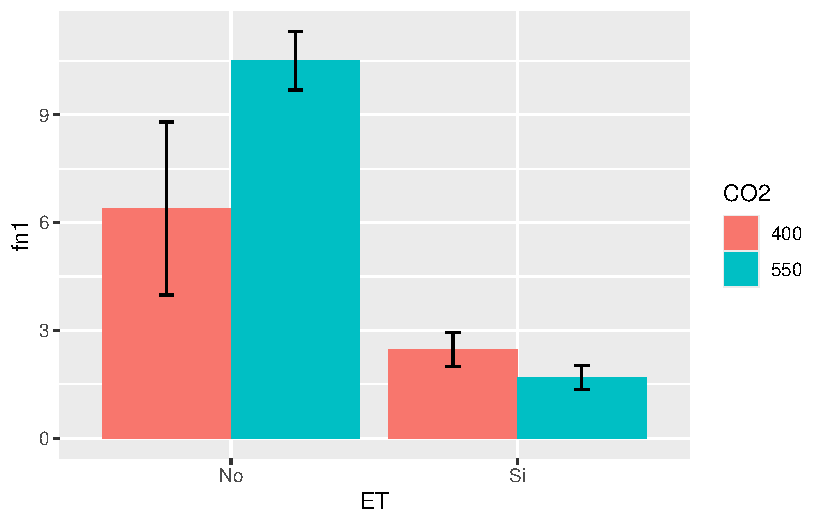
\includegraphics[width=1\textwidth,height=\textheight]{curso_R_2025_q_files/figure-pdf/unnamed-chunk-66-1.pdf}

}

\end{figure}

Una alternativa para no tener que realizar manualmente la transformación
de la base de datos cuando queremos graficar medias y desvíos es usar
\texttt{stat\_summary}. Esta función tiene una nomenclatura algo
distinta a las otras y permite especificar diferentes geoms. Veamos para
realizar el último gráfico:

\begin{Shaded}
\begin{Highlighting}[]
\FunctionTok{ggplot}\NormalTok{(SEM\_Alim, }\FunctionTok{aes}\NormalTok{(ET, PS, }\AttributeTok{fill=}\NormalTok{CO2))}\SpecialCharTok{+}
  \FunctionTok{stat\_summary}\NormalTok{(}\AttributeTok{fun=}\NormalTok{mean, }\AttributeTok{geom=}\StringTok{"col"}\NormalTok{,}
               \AttributeTok{position =} \FunctionTok{position\_dodge}\NormalTok{(}\FloatTok{0.9}\NormalTok{)) }\SpecialCharTok{+}
  \FunctionTok{stat\_summary}\NormalTok{(}\AttributeTok{fun.data=}\NormalTok{mean\_se, }\AttributeTok{geom =}\StringTok{\textquotesingle{}errorbar\textquotesingle{}}\NormalTok{, }\AttributeTok{width=}\FloatTok{0.2}\NormalTok{,}
               \AttributeTok{position =} \FunctionTok{position\_dodge}\NormalTok{(}\FloatTok{0.9}\NormalTok{))}
\end{Highlighting}
\end{Shaded}

Sin embargo, si queremos agregar las letras del Tukey realizado, será
más adecuado hacerlo con el cálculo previo de medias y error estándar.
Esto es así ya que nos permite ubicar adecuadamente las letras en la
altura correspondiente a cada columna. Las letras las incorporaremos de
forma manual con un nuevo geom, el \emph{geom\_text}:

\begin{Shaded}
\begin{Highlighting}[]
\NormalTok{G3 }\SpecialCharTok{+} \FunctionTok{geom\_text}\NormalTok{(}\FunctionTok{aes}\NormalTok{(}\AttributeTok{y =}\NormalTok{ fn1 }\SpecialCharTok{+}\NormalTok{ fn2,}
                \AttributeTok{label=} \FunctionTok{c}\NormalTok{(}\StringTok{"ab"}\NormalTok{, }\StringTok{"b"}\NormalTok{, }\StringTok{"a"}\NormalTok{, }\StringTok{"b"}\NormalTok{)),}
                \AttributeTok{position=}\FunctionTok{position\_dodge}\NormalTok{(}\FloatTok{0.9}\NormalTok{),}
                \AttributeTok{vjust=}\SpecialCharTok{{-}}\NormalTok{.}\DecValTok{5}\NormalTok{) }\CommentTok{\# ajuste vertical de la posición}
\end{Highlighting}
\end{Shaded}

\begin{figure}[H]

{\centering 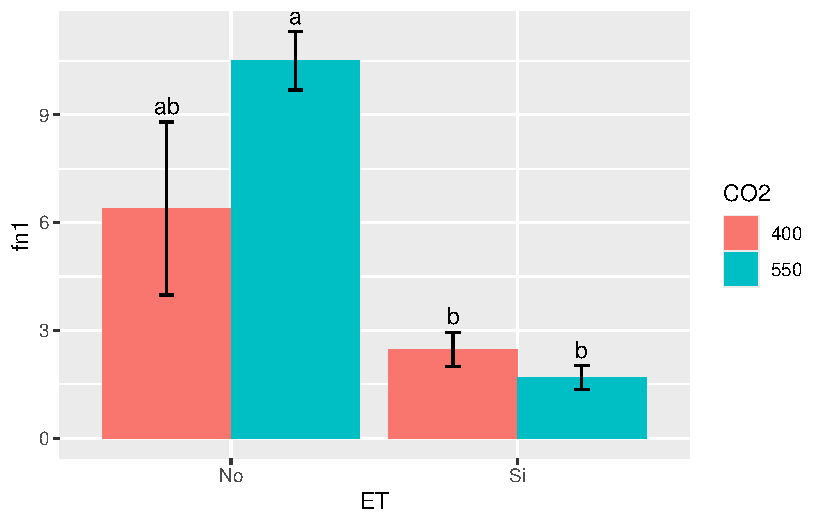
\includegraphics[width=1\textwidth,height=\textheight]{curso_R_2025_q_files/figure-pdf/unnamed-chunk-68-1.pdf}

}

\end{figure}

\hypertarget{gruxe1fico-de-barras-apiladas-y-apilado-porcentual}{%
\subsubsection{Gráfico de barras apiladas y apilado
porcentual}\label{gruxe1fico-de-barras-apiladas-y-apilado-porcentual}}

Veremos ahora cómo realizar un gráfico de barras apilado y un apilado
porcentual. Supongamos como ejemplo que queremos graficar el peso seco
de los órganos evaluados en plantas de soja de la variedad Alim 3,14.
Para ello, lo primero que debemos hacer es ``ordenar'' los niveles del
factor como los queramos mostrar. En nuestro caso, iremos de abajo hacia
arriba de la planta:

\begin{Shaded}
\begin{Highlighting}[]
\NormalTok{ALIM}\SpecialCharTok{$}\NormalTok{Organo }\OtherTok{\textless{}{-}} \FunctionTok{factor}\NormalTok{(ALIM}\SpecialCharTok{$}\NormalTok{Organo, }
                        \AttributeTok{levels =} \FunctionTok{c}\NormalTok{(}\StringTok{"Tallo"}\NormalTok{,}\StringTok{"Hoja"}\NormalTok{,}\StringTok{"Vaina"}\NormalTok{,}\StringTok{"Semilla"}\NormalTok{)) }
\end{Highlighting}
\end{Shaded}

Una vez hecho esto, vamos a transformar nuestra base de datos utilizando
la función \texttt{ddply}del paquete \textbf{plyr}. Esta función tiene
un uso particular que excede el contenido de este curso, veremos
simplemente cómo utilizarla con el ejemplo:

\begin{Shaded}
\begin{Highlighting}[]
\FunctionTok{library}\NormalTok{(plyr)}
\NormalTok{ALIM\_apilado }\OtherTok{\textless{}{-}}\NormalTok{ ALIM }\SpecialCharTok{\%\textgreater{}\%} \FunctionTok{select}\NormalTok{(Organo, ET, PS) }\SpecialCharTok{\%\textgreater{}\%} 
  \FunctionTok{group\_by}\NormalTok{(ET, Organo) }\SpecialCharTok{\%\textgreater{}\%} 
  \FunctionTok{summarise\_all}\NormalTok{(}\FunctionTok{funs}\NormalTok{(mean,se)) }\SpecialCharTok{\%\textgreater{}\%} 
  \FunctionTok{ddply}\NormalTok{(}\FunctionTok{c}\NormalTok{(}\StringTok{"ET"}\NormalTok{), transform,}
        \AttributeTok{percent\_PS =}\NormalTok{  mean}\SpecialCharTok{/} \FunctionTok{sum}\NormalTok{(mean) }\SpecialCharTok{*} \DecValTok{100}\NormalTok{) }\SpecialCharTok{\%\textgreater{}\%} 
  \FunctionTok{ddply}\NormalTok{(}\FunctionTok{c}\NormalTok{(}\StringTok{"ET"}\NormalTok{), transform, }\AttributeTok{label\_y=}\FunctionTok{cumsum}\NormalTok{(mean)) }\SpecialCharTok{\%\textgreater{}\%} 
  \FunctionTok{ddply}\NormalTok{(}\FunctionTok{c}\NormalTok{(}\StringTok{"ET"}\NormalTok{), transform, }\AttributeTok{label\_y\_perc=}\FunctionTok{cumsum}\NormalTok{(percent\_PS)) }\SpecialCharTok{\%\textgreater{}\%} 
  \FunctionTok{mutate}\NormalTok{(}\AttributeTok{Organo=}\FunctionTok{factor}\NormalTok{(Organo, }
                       \AttributeTok{levels=}\FunctionTok{c}\NormalTok{(}\StringTok{"Semilla"}\NormalTok{, }\StringTok{"Vaina"}\NormalTok{,}
                                             \StringTok{"Hoja"}\NormalTok{, }\StringTok{"Tallo"}\NormalTok{)))}
\CommentTok{\# notar que volvemos a invertir el orden  }
\end{Highlighting}
\end{Shaded}

\begin{longtable}[]{@{}llrrrrr@{}}
\toprule\noalign{}
ET & Organo & mean & se & percent\_PS & label\_y & label\_y\_perc \\
\midrule\noalign{}
\endhead
\bottomrule\noalign{}
\endlastfoot
No & Tallo & 4.680000 & 0.5586889 & 17.18587 & 4.68000 & 17.18587 \\
No & Hoja & 9.740000 & 0.9862048 & 35.76718 & 14.42000 & 52.95306 \\
No & Vaina & 4.365000 & 0.7491584 & 16.02913 & 18.78500 & 68.98219 \\
No & Semilla & 8.446667 & 1.4605996 & 31.01781 & 27.23167 & 100.00000 \\
\end{longtable}

Como se puede ver, además de calcular media y error estándar, se crearon
las variables label\_y (que nos da el acumulado parcial, nos servirá
como posición para poner una etiqueta) y label\_y\_perc para el
acumulado porcentual. Ahora podemos ejecutar los gráficos y agregar
además el valor de cada columna apilada:

\begin{Shaded}
\begin{Highlighting}[]
\NormalTok{G4 }\OtherTok{\textless{}{-}}\NormalTok{ ALIM\_apilado }\SpecialCharTok{\%\textgreater{}\%}   
\FunctionTok{ggplot}\NormalTok{(}\FunctionTok{aes}\NormalTok{(ET, mean, }\AttributeTok{fill=}\NormalTok{Organo))}\SpecialCharTok{+}
  \FunctionTok{geom\_col}\NormalTok{() }\SpecialCharTok{+}
  \FunctionTok{geom\_text}\NormalTok{(}\FunctionTok{aes}\NormalTok{(}\AttributeTok{label=}\FunctionTok{round}\NormalTok{(mean, }\DecValTok{2}\NormalTok{), }\CommentTok{\# agregamos el valor}
                \AttributeTok{y =}\NormalTok{ label\_y))  }\CommentTok{\# indica la posición}
\NormalTok{G4}
\end{Highlighting}
\end{Shaded}

\begin{figure}[H]

{\centering 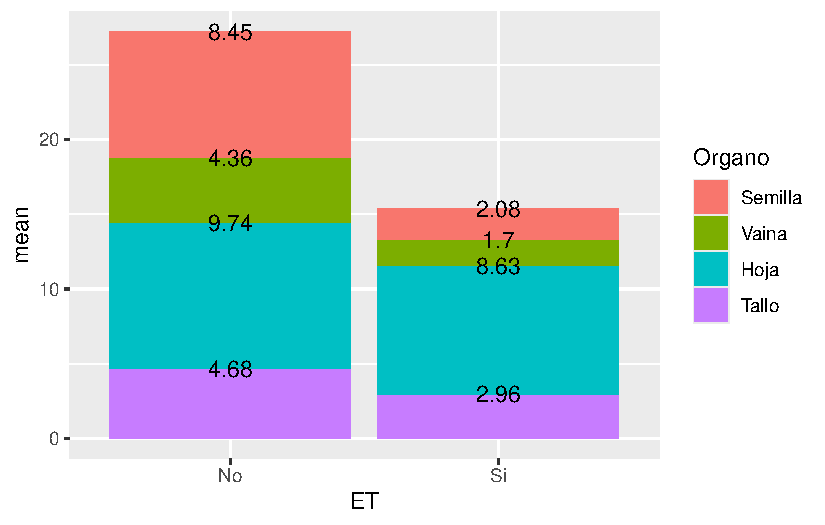
\includegraphics{curso_R_2025_q_files/figure-pdf/unnamed-chunk-71-1.pdf}

}

\end{figure}

\begin{Shaded}
\begin{Highlighting}[]
\NormalTok{G5 }\OtherTok{\textless{}{-}}\NormalTok{ ALIM\_apilado }\SpecialCharTok{\%\textgreater{}\%}   
  \FunctionTok{ggplot}\NormalTok{(}\FunctionTok{aes}\NormalTok{(ET, percent\_PS, }\AttributeTok{fill=}\NormalTok{Organo))}\SpecialCharTok{+}
  \FunctionTok{geom\_col}\NormalTok{() }\SpecialCharTok{+}
  \FunctionTok{geom\_text}\NormalTok{(}\FunctionTok{aes}\NormalTok{(}\AttributeTok{label=}\FunctionTok{round}\NormalTok{(percent\_PS, }\DecValTok{2}\NormalTok{), }\AttributeTok{y =}\NormalTok{ label\_y\_perc), }\AttributeTok{vjust=}\DecValTok{2}\NormalTok{)}
\NormalTok{G5}
\end{Highlighting}
\end{Shaded}

\begin{figure}[H]

{\centering 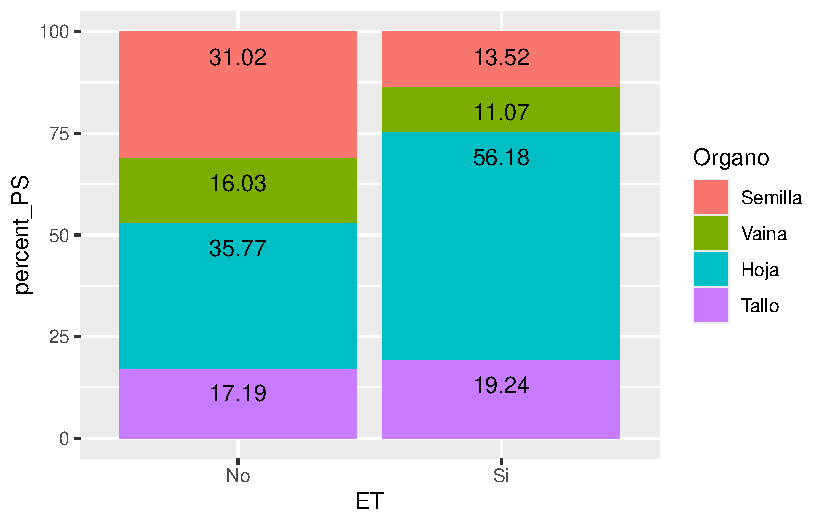
\includegraphics{curso_R_2025_q_files/figure-pdf/unnamed-chunk-71-2.pdf}

}

\end{figure}

\hypertarget{boxplot}{%
\subsection{Boxplot}\label{boxplot}}

Los gráficos tipo boxplot también son formas frecuentes de presentar
variables numéricas con distintos factores de clasificación. Veremos
algunas formas de hacerlo.

\hypertarget{funciuxf3n-boxplot}{%
\subsubsection{Función boxplot}\label{funciuxf3n-boxplot}}

La función derivada de \texttt{plot} para hacer gráficos de barras es
\texttt{boxplot}. Se utiliza de forma similar a los gráficos ya vistos:

\begin{Shaded}
\begin{Highlighting}[]
\FunctionTok{boxplot}\NormalTok{(PS}\SpecialCharTok{\textasciitilde{}}\NormalTok{ET, }\AttributeTok{data =}\NormalTok{ SEM\_Alim,}
        \AttributeTok{ylim =} \FunctionTok{c}\NormalTok{(}\DecValTok{0}\NormalTok{,}\DecValTok{12}\NormalTok{),}
        \AttributeTok{xlab=}\StringTok{"Estrés térmico"}\NormalTok{,}
        \AttributeTok{ylab=} \StringTok{"Peso seco"}\NormalTok{,}
        \AttributeTok{las=}\DecValTok{1}\NormalTok{, }\AttributeTok{cex.axis=}\FloatTok{0.8}\NormalTok{)}
\end{Highlighting}
\end{Shaded}

\begin{figure}[H]

{\centering 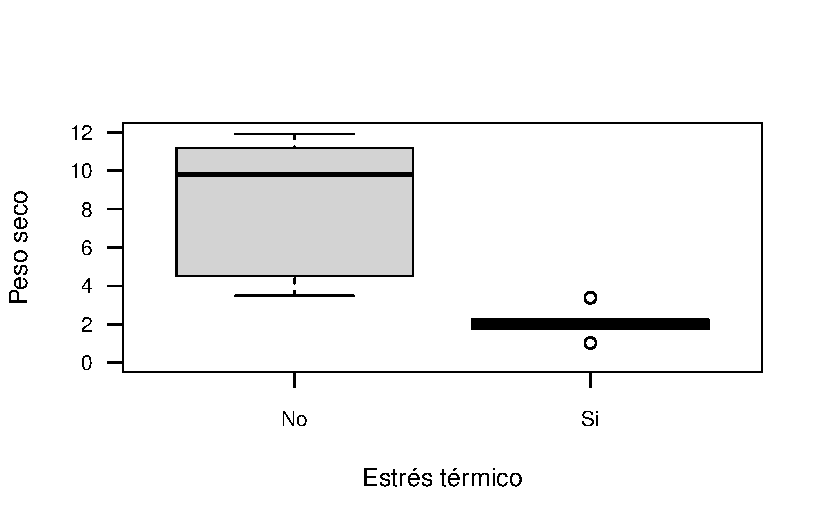
\includegraphics[width=1\textwidth,height=\textheight]{curso_R_2025_q_files/figure-pdf/unnamed-chunk-72-1.pdf}

}

\end{figure}

\hypertarget{geom_boxplot}{%
\subsubsection{geom\_boxplot}\label{geom_boxplot}}

El paquete \textbf{ggplot2} nos ofrece una vez maś una forma muy
versátil de crear gráficos de cajas. La función en cuestión es
\texttt{geom\_boxplot} que, a diferencias de \texttt{geom\_col}, no
requiere que realicemos ningún cálculo previo. De esta manera podemos
generar un gráfico con un par de líneas de código:

\begin{Shaded}
\begin{Highlighting}[]
\FunctionTok{ggplot}\NormalTok{(SEM\_Alim, }\FunctionTok{aes}\NormalTok{(ET, PS))}\SpecialCharTok{+}
  \FunctionTok{geom\_boxplot}\NormalTok{()}
\end{Highlighting}
\end{Shaded}

\begin{figure}[H]

{\centering 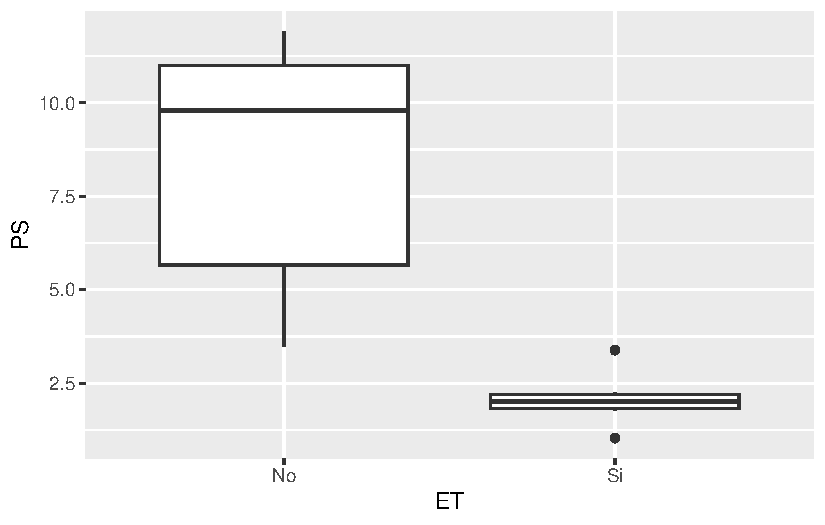
\includegraphics[width=1\textwidth,height=\textheight]{curso_R_2025_q_files/figure-pdf/unnamed-chunk-73-1.pdf}

}

\end{figure}

Si vemos con atención a este gráfico le faltan una serie de cosas que
podrían mejorarlo. Por un lado, los extremos de los cuartiles no tienen
la marca de final, sino que simplemente termina la línea. Sumado a esto,
podría interesarnos agregar el valor de la media, que no figura en el
gráfico. Veamos como incorporarlos con la función ya vista
\texttt{stat\_summary}:

\begin{Shaded}
\begin{Highlighting}[]
\FunctionTok{ggplot}\NormalTok{(SEM\_Alim, }\FunctionTok{aes}\NormalTok{(ET, PS))}\SpecialCharTok{+}
  \FunctionTok{stat\_boxplot}\NormalTok{(}\AttributeTok{geom =}\StringTok{\textquotesingle{}errorbar\textquotesingle{}}\NormalTok{, }\AttributeTok{width=}\FloatTok{0.2}\NormalTok{)}\SpecialCharTok{+} \CommentTok{\#debemos colocarlo primero para que quede al fondo}
  \FunctionTok{geom\_boxplot}\NormalTok{() }\SpecialCharTok{+}
  \FunctionTok{stat\_summary}\NormalTok{(}\AttributeTok{fun=}\NormalTok{mean, }\AttributeTok{geom=}\StringTok{"point"}\NormalTok{)}
\end{Highlighting}
\end{Shaded}

\begin{figure}[H]

{\centering 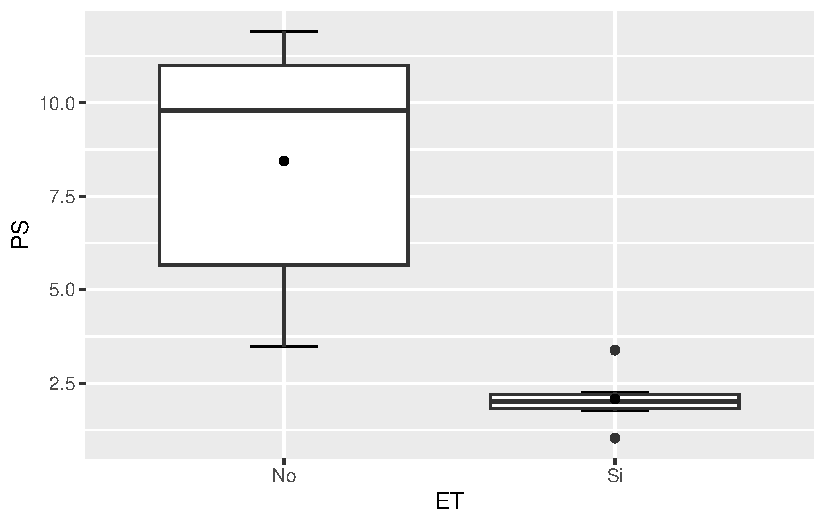
\includegraphics[width=1\textwidth,height=\textheight]{curso_R_2025_q_files/figure-pdf/unnamed-chunk-74-1.pdf}

}

\end{figure}

\hypertarget{actividad-5}{%
\subsection{Actividad 5}\label{actividad-5}}

Realice un gráfico de barras y un gráfico de cajas donde demuestre los
resultados de los ANOVA realizados en la actividad 4.

\href{../}{Volver al inicio}

\hypertarget{unidad-4.-estructura-y-estuxe9tica-de-gruxe1ficos-con-ggplot2.}{%
\section{Unidad 4. Estructura y estética de gráficos con
ggplot2.}\label{unidad-4.-estructura-y-estuxe9tica-de-gruxe1ficos-con-ggplot2.}}

En esta unidad veremos una serie de contenidos relacionados con
parámetros estructurales del gráfico (como las escalas, la división de
la ventana gráfica, etc.) y estéticos que van desde la paleta de colores
utilizada hasta el tema general.

Sin embargo, empezaremos viendo cómo exportar un gráfico para luego
poder ir extrayendo los que iremos generando.

\hypertarget{exportaciuxf3n-de-resultados-y-gruxe1ficos}{%
\subsection{Exportación de resultados y
gráficos}\label{exportaciuxf3n-de-resultados-y-gruxe1ficos}}

\hypertarget{exportaciuxf3n-de-datos}{%
\subsubsection{Exportación de datos}\label{exportaciuxf3n-de-datos}}

A este respecto, en mi práctica personal suelo leer los resultados desde
la consola de R y, de ser necesario, realizo el pasaje manualmente de la
información que me resulte de interés a un excel para su almacenamiento.
De todas maneras, existen maneras de exportar diferentes formatos de
archivos desde R. Cuando lo considero necesario, utilizo archivos del
tipo csv. Así por ejemplo para exportar los datos de una regresión:

\begin{Shaded}
\begin{Highlighting}[]
\NormalTok{REG }\OtherTok{\textless{}{-}} \FunctionTok{summary}\NormalTok{(fit1) }\CommentTok{\# creamos un objeto para poder después extraer los coeficientes}

\FunctionTok{write.csv2}\NormalTok{(REG}\SpecialCharTok{$}\NormalTok{coefficients, }\StringTok{"regresión prueba.csv"}\NormalTok{)}
\end{Highlighting}
\end{Shaded}

Como vemos, debo tener una tabla limpia y luego agregar el nombre y
formato del archivo a crear. Lo mismo si quisiera extraer la tabla de un
anova o un tukey:

\begin{Shaded}
\begin{Highlighting}[]
\FunctionTok{write.csv2}\NormalTok{(}\FunctionTok{anova}\NormalTok{(fit3), }\StringTok{"anova prueba.csv"}\NormalTok{)}
\FunctionTok{write.csv2}\NormalTok{(tukey3}\SpecialCharTok{$}\NormalTok{groups, }\StringTok{"tukey prueba2.csv"}\NormalTok{)}
\end{Highlighting}
\end{Shaded}

Por supuesto, todo lo que exportemos se guardará en el directorio
seteado al comienzo con setwd().

\hypertarget{exportaciuxf3n-de-gruxe1ficos}{%
\subsubsection{Exportación de
gráficos}\label{exportaciuxf3n-de-gruxe1ficos}}

Este apartado es mucho más útil que el anterior y nos va a permitir
extraer nuestras figuras que hayamos creado de una forma adecuada.
Veremos 3 formas de exportar un gráfico.

\hypertarget{interfaz-gruxe1fica-de-rstudio}{%
\paragraph{Interfaz gráfica de
RStudio}\label{interfaz-gruxe1fica-de-rstudio}}

En la ventana 4 de RStudio se nos muestran los gráficos que hayamos
generado. En la barra superior de esa ventana (siempre que estemos en la
pestaña \emph{Plots}) veremos la opción de \emph{Export}. Si allí
entramos en \emph{Save as image} nos brinda una serie de opciones de
exportación. Menciono esta posibilidad porque en algunos contextos puede
sernos de utilidad. Como siempre que utilizamos la interfaz gráfica,
esta tiene la desventaja de no nos deja ningún tipo de registro de lo
que hayamos hecho, lo que no nos permite repetir la exportación en
igualdad de condiciones, si es que fuera necesario.

\hypertarget{devices}{%
\paragraph{Devices}\label{devices}}

Una segunda opción es el uso de Devices. Esta opción consiste en un
código inicial donde definimos el formato, luego el gráfico y finalmente
el cierre. Así por ejemplo para exportar un jpg:

\begin{Shaded}
\begin{Highlighting}[]
\FunctionTok{jpeg}\NormalTok{(}\AttributeTok{file =} \StringTok{"mi\_grafico.jpg"}\NormalTok{,}
      \AttributeTok{width =} \DecValTok{12}\NormalTok{, }\AttributeTok{height =} \DecValTok{10}\NormalTok{, }\CommentTok{\#ancho y alto}
     \AttributeTok{quality =} \DecValTok{95}\NormalTok{, }\CommentTok{\#grado de no{-}compresión}
     \AttributeTok{res =} \DecValTok{300}\NormalTok{) }\CommentTok{\#resolución en puntos por pulgada}
\FunctionTok{boxplot}\NormalTok{(PS}\SpecialCharTok{\textasciitilde{}}\NormalTok{ET,}
        \AttributeTok{data =}\NormalTok{ SEM\_Alim) }\CommentTok{\# comandos gráficos}
\FunctionTok{dev.off}\NormalTok{() }\CommentTok{\# cerrar el gráfico}
\end{Highlighting}
\end{Shaded}

También es posible exportar en PDF, SVG (formato vectorizado), y otros.
Es recomendable pintar todo el texto (inicio + gráfico + cierre) y luego
ejecutar todo como una única corrida.

\hypertarget{ggsave}{%
\paragraph{ggsave}\label{ggsave}}

Esta es una opción interna dentro del entorno de \textbf{ggplot2}. Se
debe ejecutar a continuación y luego de haber corrido el gráfico. Su
estructura es la siguiente:

\begin{Shaded}
\begin{Highlighting}[]
\FunctionTok{ggsave}\NormalTok{(}\StringTok{"mi gráfico.png"}\NormalTok{, }\CommentTok{\# nombre y formato}
       \AttributeTok{width =} \ConstantTok{NA}\NormalTok{, }\AttributeTok{height =} \ConstantTok{NA}\NormalTok{, }\CommentTok{\# ancho y alto, si no especificamos se ve tal cual en la ventana 4}
       \AttributeTok{dpi =} \DecValTok{300}\NormalTok{) }\CommentTok{\# resolución}
\end{Highlighting}
\end{Shaded}

Si se quiere exportar en formato SVG, es necesaria la instalación del
paquete \emph{svglite}.

\hypertarget{tuxedtulos}{%
\subsection{Títulos}\label{tuxedtulos}}

Para modificar los títulos de nuestros gráficos utilizaremos el
parámetro \emph{labs}. Allí modificaremos la etiqueta de cada eje, de la
leyenda, y posibles títulos del gráfico.

\begin{Shaded}
\begin{Highlighting}[]
\NormalTok{G3 }\OtherTok{\textless{}{-}}\NormalTok{ G3 }\SpecialCharTok{+}
  \FunctionTok{labs}\NormalTok{(}\AttributeTok{x =} \StringTok{"Estrés térmico"}\NormalTok{, }
       \AttributeTok{y =} \StringTok{"Peso seco (g)"}\NormalTok{, }
       \AttributeTok{fill =} \FunctionTok{expression}\NormalTok{(CO[}\DecValTok{2}\NormalTok{]), }\CommentTok{\# cambia la leyenda}
       \AttributeTok{title =} \StringTok{"Peso seco de semillas de soja"}\NormalTok{) ; G3}
\end{Highlighting}
\end{Shaded}

\begin{figure}[H]

{\centering 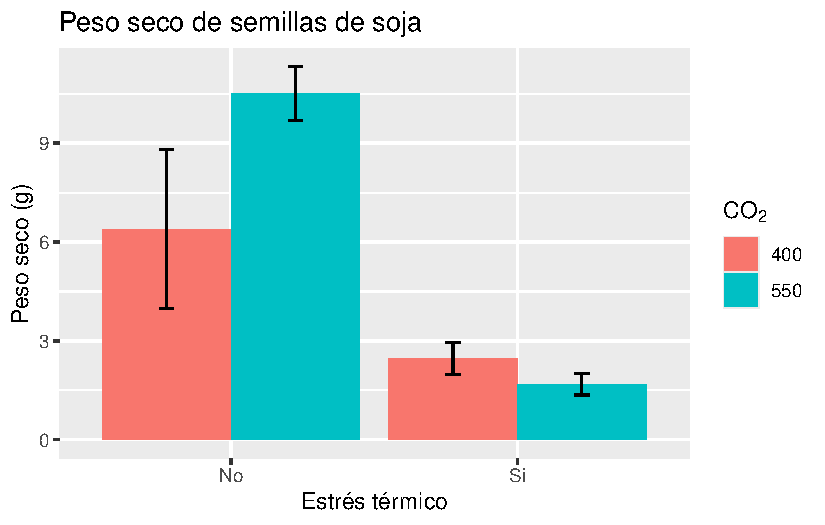
\includegraphics[width=1\textwidth,height=\textheight]{curso_R_2025_q_files/figure-pdf/unnamed-chunk-79-1.pdf}

}

\end{figure}

\hypertarget{scales}{%
\subsection{Scales}\label{scales}}

\hypertarget{manipulando-los-ejes}{%
\subsubsection{Manipulando los ejes}\label{manipulando-los-ejes}}

Podemos establecer la estructura de nuestros ejes a partir de los
comandos \texttt{scale\_x\_***} donde en debemos indicar el tipo de dato
de nuestro eje (todo esto es válido tanto para el eje \emph{x} como el
\emph{y}). Así dependiendo del tipo de variable, serán los datos a
modificar. Por ejemplo si la variable es continua:

\begin{Shaded}
\begin{Highlighting}[]
\NormalTok{  ... }\SpecialCharTok{+}
  \FunctionTok{scale\_x\_continuos}\NormalTok{(}\AttributeTok{expand =} \FunctionTok{c}\NormalTok{(}\DecValTok{0}\NormalTok{,}\DecValTok{0}\NormalTok{), }\CommentTok{\# estable la ubicación en el eje}
                    \AttributeTok{limits=}\FunctionTok{c}\NormalTok{(inferior,superior), }\CommentTok{\# entre qué valores se graficará}
                    \AttributeTok{breaks =} \FunctionTok{seq}\NormalTok{(inferior,superior, }\CommentTok{\# entre qué valores se mostrará la escala}
                                 \AttributeTok{by =}\NormalTok{ número)) }\CommentTok{\# cada cuánto habrá cortes}
\end{Highlighting}
\end{Shaded}

Es importante destacar que el parámetro \emph{limits} establece los
límites del gráfico y los valores que se tomarán en cuenta. Si algo de
nuestros datos excede ese valor, no será considerado para el gráfico. Si
en cambio queremos tomar en cuenta todos los datos pero hacer un recorte
en el gráfico, debemos usar el comando
\texttt{coord\_cartesian(ylim=c(inferior,superior))} en una nueva línea.

En el caso de querer modificar los nombres que aparecen en el eje
(habitualmente para variables discretas o categóricas) usaremos el
comando \texttt{labels}:

\begin{Shaded}
\begin{Highlighting}[]
\FunctionTok{scale\_x\_discrete}\NormalTok{(}\AttributeTok{labels =} \FunctionTok{c}\NormalTok{(etiqueta1, etiqueta2, ...))}
\end{Highlighting}
\end{Shaded}

Continuando con nuestro ejemplo en el G3, comparemos con y sin
manipulación de ejes:

\begin{Shaded}
\begin{Highlighting}[]
\NormalTok{G3}
\NormalTok{G3 }\OtherTok{\textless{}{-}}\NormalTok{ G3 }\SpecialCharTok{+} \FunctionTok{scale\_x\_discrete}\NormalTok{(}\AttributeTok{labels =} \FunctionTok{c}\NormalTok{(}\StringTok{"Sin ET"}\NormalTok{, }\StringTok{"Con ET"}\NormalTok{)) }\SpecialCharTok{+}
  \FunctionTok{scale\_y\_continuous}\NormalTok{(}\AttributeTok{expand =} \FunctionTok{c}\NormalTok{(}\DecValTok{0}\NormalTok{,}\DecValTok{0}\NormalTok{), }
                     \AttributeTok{limits =} \FunctionTok{c}\NormalTok{(}\DecValTok{0}\NormalTok{, }\DecValTok{12}\NormalTok{), }
                     \AttributeTok{breaks =} \FunctionTok{seq}\NormalTok{(}\DecValTok{0}\NormalTok{,}\DecValTok{12}\NormalTok{, }\AttributeTok{by=} \DecValTok{1}\NormalTok{)); G3}
\end{Highlighting}
\end{Shaded}

\begin{figure}[H]

{\centering 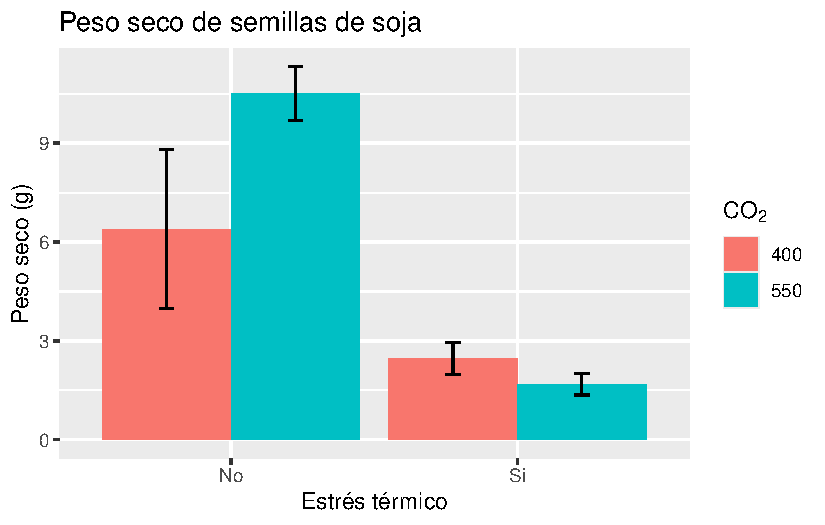
\includegraphics[width=1\textwidth,height=\textheight]{curso_R_2025_q_files/figure-pdf/unnamed-chunk-82-1.pdf}

}

\end{figure}

\begin{figure}[H]

{\centering 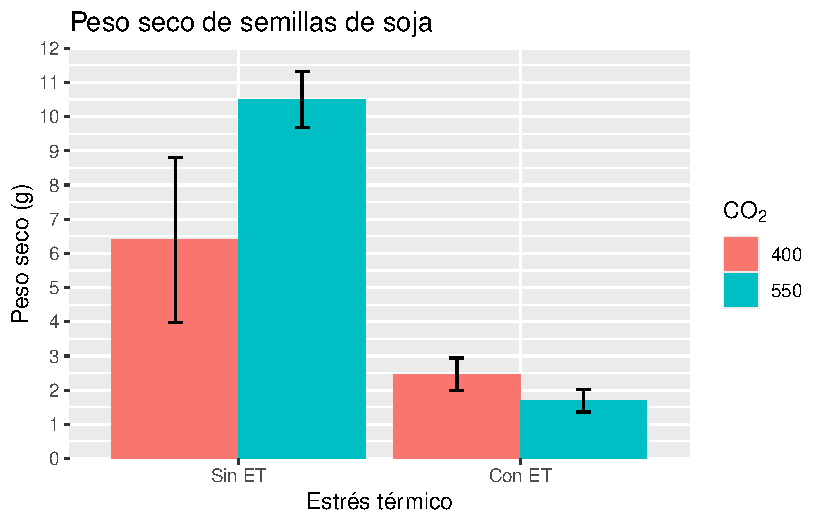
\includegraphics[width=1\textwidth,height=\textheight]{curso_R_2025_q_files/figure-pdf/unnamed-chunk-82-2.pdf}

}

\end{figure}

\hypertarget{colores}{%
\subsubsection{Colores}\label{colores}}

R permite la utilización de una gran cantidad de colores diferentes (ver
documento \emph{ColorChart}). Se pueden modificar los colores de casi
todos los objetos en un gráfico, aquí nos centraremos en contornos y
rellenos de nuestros elementos que representan los datos. Como regla
general, si nuestro geom admite relleno este se modifica con el
parámetro \emph{fill}, mientras que \emph{col} modificará el borde. Si
no se admite relleno (gráficos de líneas o puntos), solo utilizaremos
\emph{col}. Cómo modificamos los colores varía un poco según diferentes
casos:

\begin{itemize}
\item
  Si el color es el mismo para todos, se modifica dentro de los
  parámetros del geom. Por ejemplo:
  \texttt{geom\_col(col=\ "black",\ fill=\ "red")}.
\item
  Si debemos modificar el color o el relleno según un criterio de
  clasificación (es decir que seteamos el parámetro que clasifica en el
  aes()) usaremos el comando
  \texttt{scale\_colour\_manual(values=c("color1",\ "color2",\ ....))}
  para establecer manualmente los colores. Lo mismo para el relleno pero
  será
  \texttt{scale\_fill\_manual(values=c("color1",\ "color2",\ ....))}. Es
  importante destacar que la cantidad de colores debe coincidir con los
  niveles del factor en cuestión.
\end{itemize}

Veamos un ejemplo donde combinamos lo visto hasta ahora:

\begin{Shaded}
\begin{Highlighting}[]
\NormalTok{G3 }\SpecialCharTok{+} \FunctionTok{geom\_col}\NormalTok{(}\AttributeTok{col =} \StringTok{"black"}\NormalTok{, }\AttributeTok{position =} \StringTok{"dodge"}\NormalTok{) }\SpecialCharTok{+} \CommentTok{\# repetimos para cambiar el borde}
  \FunctionTok{scale\_fill\_manual}\NormalTok{(}\AttributeTok{values =} \FunctionTok{c}\NormalTok{(}\StringTok{"skyblue3"}\NormalTok{, }\StringTok{"antiquewhite2"}\NormalTok{))}
\end{Highlighting}
\end{Shaded}

\begin{figure}[H]

{\centering 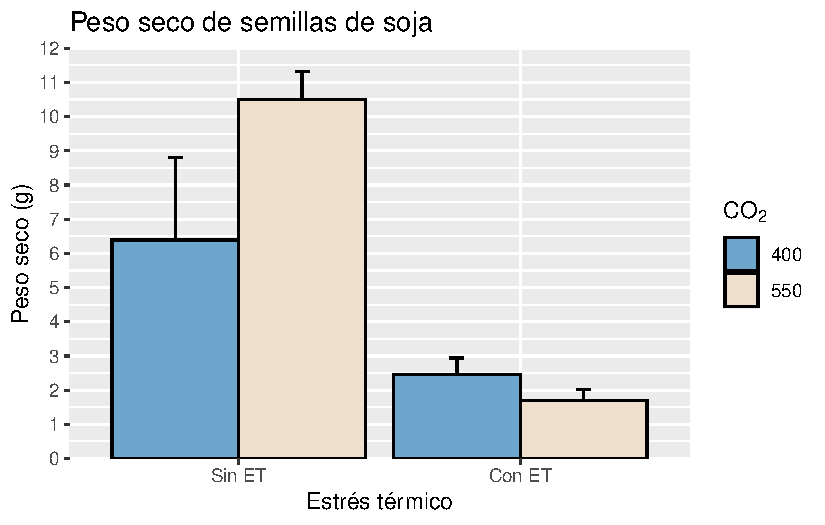
\includegraphics[width=1\textwidth,height=\textheight]{curso_R_2025_q_files/figure-pdf/unnamed-chunk-83-1.pdf}

}

\end{figure}

En estos casos decidimos establecer manualmente el color. También
podemos utilizar paletas de colores que vienen preestablecidas. Algunas
están con el R base y otras debemos cargarlas con paquetes. En este
taller veremos el uso de la paleta \textbf{viridis}, de paquete
homónimo. La función que utilizaremos es
\texttt{scale\_fill\_viridis\_d()}, donde la ``d'' refiere a discreto.
Esta escala está especialmente diseñada para que la puedan distinguir
personas daltónicas y asignará tantos colores como sean necesarios. La
escala viridis va del violeta al amarillo, podemos reducir la escala
estableciendo el comienzo y el final de la misma. Por otro lado, también
veremos el uso del paquete \emph{paletteer}, que incluye una enorme
cantidad de paletas para utilizar
(https://r-charts.com/es/paletas-colores/). Por ejemplo en el gráfico
anterior:

\begin{Shaded}
\begin{Highlighting}[]
\NormalTok{G3 }\SpecialCharTok{+} \FunctionTok{geom\_col}\NormalTok{(}\AttributeTok{col =} \StringTok{"black"}\NormalTok{, }\AttributeTok{position =} \StringTok{"dodge"}\NormalTok{) }\SpecialCharTok{+} 
  \FunctionTok{scale\_fill\_viridis\_d}\NormalTok{()}
\end{Highlighting}
\end{Shaded}

\begin{figure}[H]

{\centering 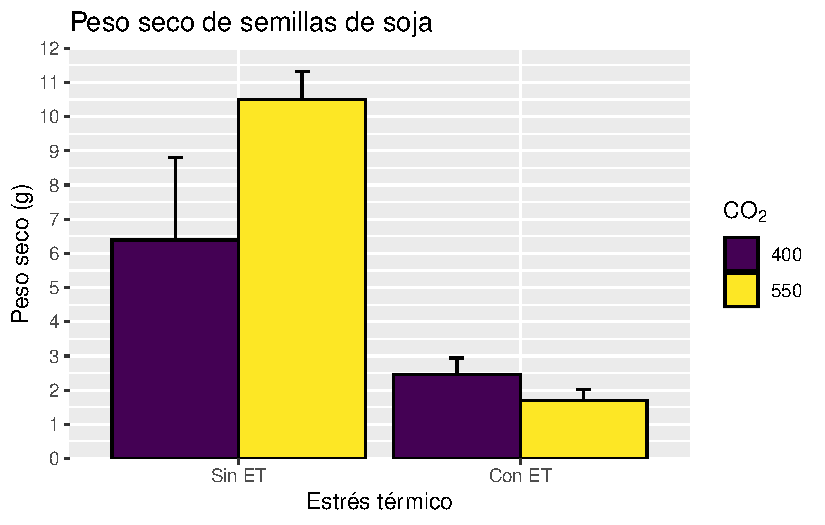
\includegraphics{curso_R_2025_q_files/figure-pdf/unnamed-chunk-84-1.pdf}

}

\end{figure}

\begin{Shaded}
\begin{Highlighting}[]
\FunctionTok{library}\NormalTok{(paletteer)}
\NormalTok{G3 }\SpecialCharTok{+} \FunctionTok{geom\_col}\NormalTok{(}\AttributeTok{col =} \StringTok{"black"}\NormalTok{, }\AttributeTok{position =} \StringTok{"dodge"}\NormalTok{) }\SpecialCharTok{+}
  \FunctionTok{scale\_fill\_manual}\NormalTok{(}\AttributeTok{values =} \FunctionTok{paletteer\_d}\NormalTok{(}\StringTok{"colorBlindness::Blue2DarkOrange12Steps"}\NormalTok{, }\DecValTok{2}\NormalTok{, }
                                         \AttributeTok{type =} \StringTok{"continuous"}\NormalTok{))}
\end{Highlighting}
\end{Shaded}

\begin{figure}[H]

{\centering 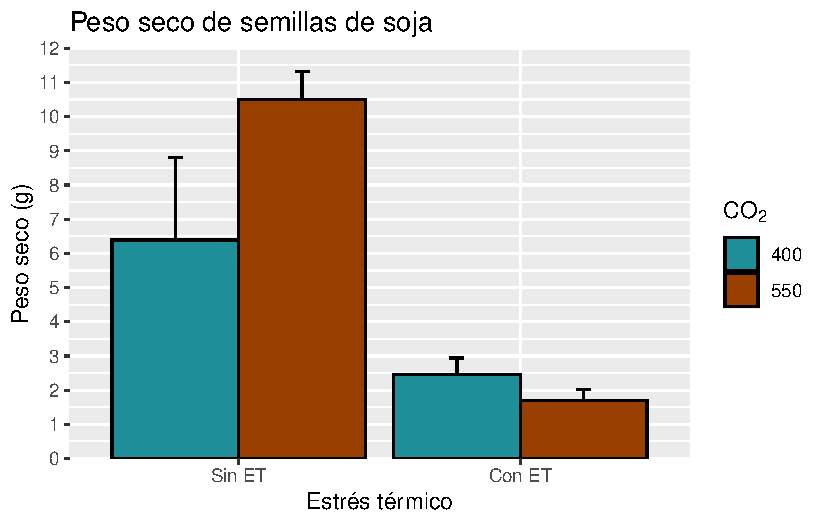
\includegraphics{curso_R_2025_q_files/figure-pdf/unnamed-chunk-84-2.pdf}

}

\end{figure}

Si queremos saber exactamente qué colores utilizó la función, podemos
utilizar la función \texttt{viridis} para nombrar los colores:

\begin{Shaded}
\begin{Highlighting}[]
\FunctionTok{library}\NormalTok{(viridis)}
\FunctionTok{viridis}\NormalTok{(}\DecValTok{2}\NormalTok{)}
\end{Highlighting}
\end{Shaded}

\begin{verbatim}
[1] "#440154FF" "#FDE725FF"
\end{verbatim}

\begin{Shaded}
\begin{Highlighting}[]
\FunctionTok{paletteer\_d}\NormalTok{(}\StringTok{"colorBlindness::Blue2DarkOrange12Steps"}\NormalTok{, }\DecValTok{2}\NormalTok{, }
                                         \AttributeTok{type =} \StringTok{"continuous"}\NormalTok{)}
\end{Highlighting}
\end{Shaded}

\begin{verbatim}
<colors>
#1E8E99FF #993F00FF 
\end{verbatim}

Nos los da con el código RGB que podemos utilizar para otros gráficos.

\hypertarget{forma-y-tipo-de-luxednea}{%
\subsubsection{Forma y tipo de línea}\label{forma-y-tipo-de-luxednea}}

Otro parámetro que puede generar diferencias entre los niveles de una
factor o que puede ser modificado para todos nuestros valores es la
forma. Para indicar el cambio se hará del mismo modo que para el color o
relleno, pero con el parámetro \texttt{shape}. Las diferentes formas se
pueden visualizar en el documento Refcard, son 25 y algunas permiten que
se les modifique el relleno. La forma puede ser combinada por el color
para enfatizar las diferencias, y originarán una sola leyenda, por
ejemplo:

\begin{Shaded}
\begin{Highlighting}[]
\FunctionTok{ggplot}\NormalTok{(HOJA,}
       \FunctionTok{aes}\NormalTok{(SPAD, Pb,}
           \AttributeTok{col =}\NormalTok{ ET,  }\CommentTok{\# clasificamos por color}
           \AttributeTok{shape =}\NormalTok{ ET)) }\SpecialCharTok{+} \CommentTok{\# y por forma}
  \FunctionTok{geom\_point}\NormalTok{(}\AttributeTok{size=} \DecValTok{5}\NormalTok{) }\SpecialCharTok{+}
  \FunctionTok{scale\_shape\_manual}\NormalTok{(}\AttributeTok{values =} \FunctionTok{c}\NormalTok{(}\DecValTok{16}\NormalTok{, }\DecValTok{18}\NormalTok{))}
\end{Highlighting}
\end{Shaded}

\begin{figure}[H]

{\centering 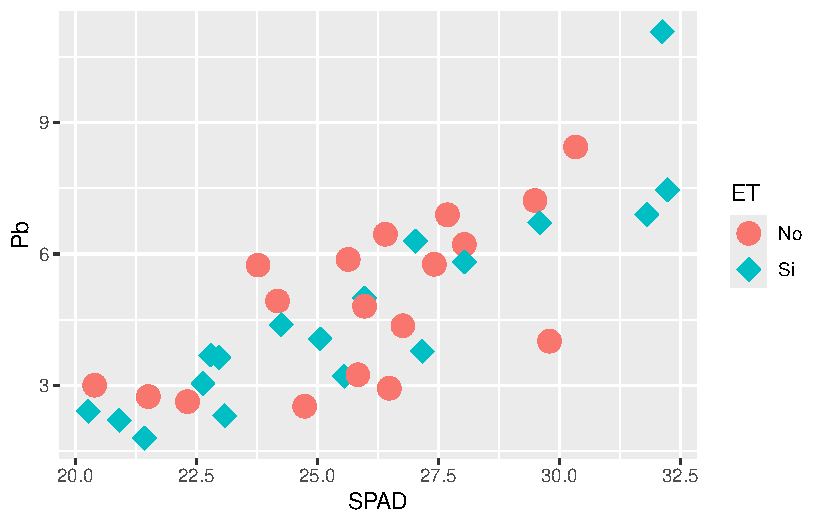
\includegraphics[width=1\textwidth,height=\textheight]{curso_R_2025_q_files/figure-pdf/unnamed-chunk-86-1.pdf}

}

\end{figure}

A su vez podemos establecer tipos de líneas en un gráfico de líneas.
Funciona de la misma manera con el parámetro \texttt{linetype}:

\begin{Shaded}
\begin{Highlighting}[]
\FunctionTok{ggplot}\NormalTok{(HOJA,}
       \FunctionTok{aes}\NormalTok{(SPAD, Pb,}
           \AttributeTok{col =}\NormalTok{ ET,}
           \AttributeTok{shape =}\NormalTok{ ET,}
           \AttributeTok{linetype =}\NormalTok{ ET)) }\SpecialCharTok{+}
  \FunctionTok{geom\_point}\NormalTok{(}\AttributeTok{size=} \DecValTok{5}\NormalTok{) }\SpecialCharTok{+}
  \FunctionTok{geom\_line}\NormalTok{()}\SpecialCharTok{+}
  \FunctionTok{scale\_shape\_manual}\NormalTok{(}\AttributeTok{values =} \FunctionTok{c}\NormalTok{(}\DecValTok{16}\NormalTok{, }\DecValTok{18}\NormalTok{)) }\SpecialCharTok{+}
  \FunctionTok{labs}\NormalTok{(}\AttributeTok{col =} \StringTok{"Estrés }\SpecialCharTok{\textbackslash{}n}\StringTok{térmico"}\NormalTok{, }
       \AttributeTok{shape =} \StringTok{"Estrés }\SpecialCharTok{\textbackslash{}n}\StringTok{térmico"}\NormalTok{, }
       \AttributeTok{linetype =} \StringTok{"Estrés }\SpecialCharTok{\textbackslash{}n}\StringTok{térmico"}\NormalTok{)}
\end{Highlighting}
\end{Shaded}

\begin{figure}[H]

{\centering 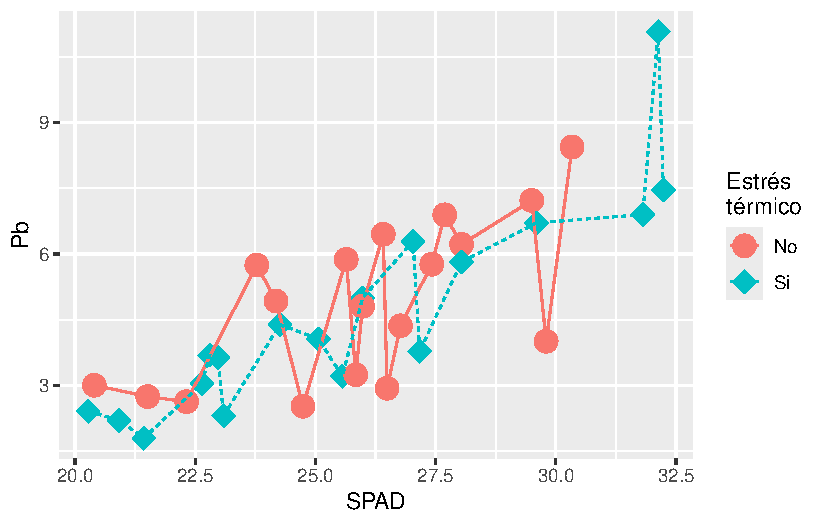
\includegraphics[width=1\textwidth,height=\textheight]{curso_R_2025_q_files/figure-pdf/unnamed-chunk-87-1.pdf}

}

\end{figure}

Como vemos, como todos los parámetros de clasificación responden al
mismo factor, la leyenda es una sola. Para modificar el título de la
leyenda se debe indicar el cambio para todos los parámetros
involucrados.

También se puede clasificar por tamaño en el caso de una variable
continua, generará una escala automática.

\begin{Shaded}
\begin{Highlighting}[]
\FunctionTok{ggplot}\NormalTok{(HOJA,}
       \FunctionTok{aes}\NormalTok{(SPAD, Pb,}
           \AttributeTok{size =}\NormalTok{ Pb, }\CommentTok{\# genera una escala discreta de tamaños }
           \AttributeTok{col =}\NormalTok{ Pb)) }\SpecialCharTok{+} \CommentTok{\# genera una escala continua de color}
  \FunctionTok{geom\_point}\NormalTok{()}
\end{Highlighting}
\end{Shaded}

\begin{figure}[H]

{\centering 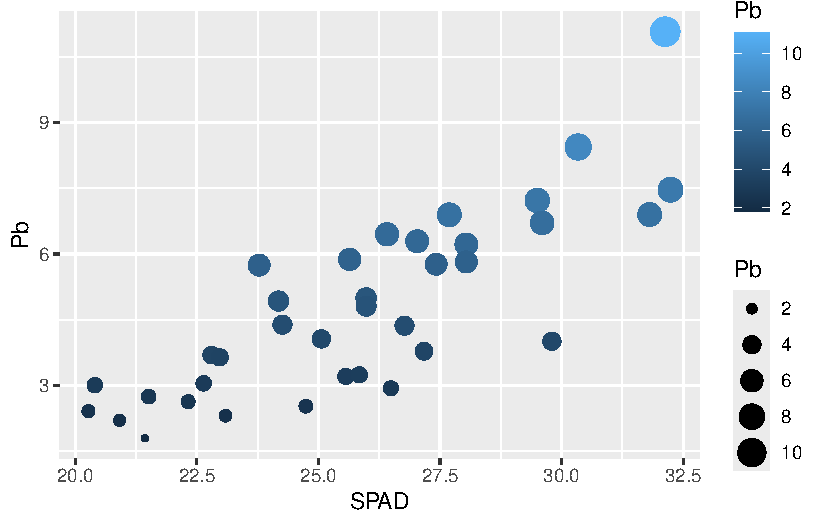
\includegraphics[width=1\textwidth,height=\textheight]{curso_R_2025_q_files/figure-pdf/unnamed-chunk-88-1.pdf}

}

\end{figure}

\hypertarget{subdivisiuxf3n-del-gruxe1fico-con-faceting}{%
\subsection{Subdivisión del gráfico con
faceting}\label{subdivisiuxf3n-del-gruxe1fico-con-faceting}}

Si nuestro gráfico requiere la subdivisión por varios factores, además
de por colores podemos dividir la ventana con faceting. El parámetro
facet\_grid requiere que introduzcamos por cuál/es variable/s se
dividirá, por lo tanto toma la forma var1\textasciitilde var2, si solo
hay una se reemplaza la faltante por un punto (.). Es importante
destacar que todas las divisiones responderán a la misma escala. Así por
ejemplo:

\begin{Shaded}
\begin{Highlighting}[]
\NormalTok{G2 }\SpecialCharTok{+} \FunctionTok{facet\_grid}\NormalTok{(.}\SpecialCharTok{\textasciitilde{}}\NormalTok{GT) }\CommentTok{\# para dividir verticalmente}
\end{Highlighting}
\end{Shaded}

\begin{figure}[H]

{\centering 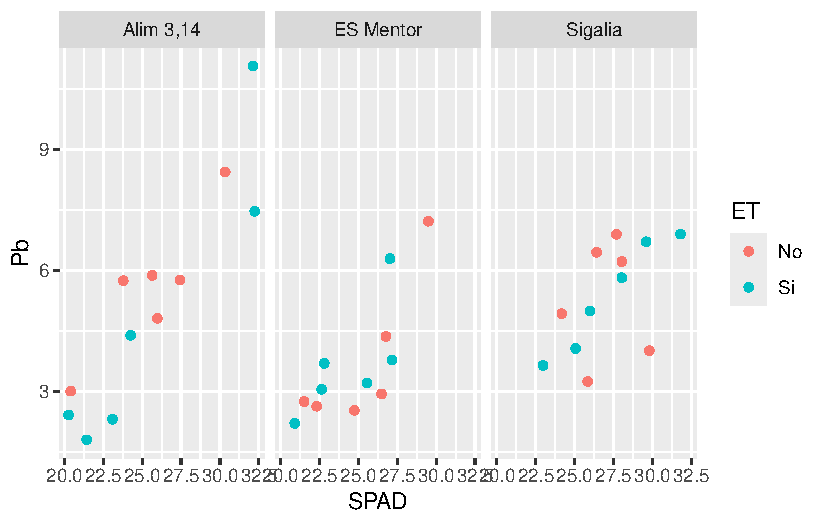
\includegraphics{curso_R_2025_q_files/figure-pdf/unnamed-chunk-89-1.pdf}

}

\end{figure}

\begin{Shaded}
\begin{Highlighting}[]
\NormalTok{G2 }\SpecialCharTok{+} \FunctionTok{facet\_grid}\NormalTok{(GT}\SpecialCharTok{\textasciitilde{}}\NormalTok{.) }\CommentTok{\# para dividir horizontalmente}
\end{Highlighting}
\end{Shaded}

\begin{figure}[H]

{\centering 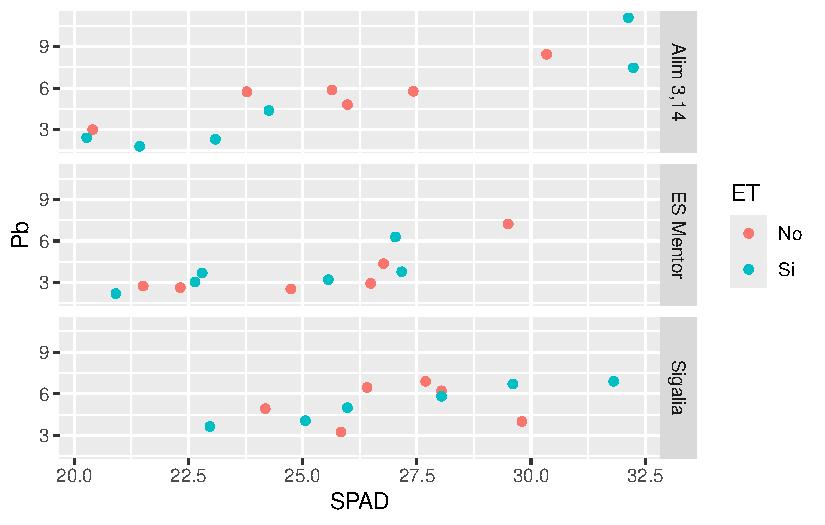
\includegraphics{curso_R_2025_q_files/figure-pdf/unnamed-chunk-89-2.pdf}

}

\end{figure}

\begin{Shaded}
\begin{Highlighting}[]
\NormalTok{G2 }\SpecialCharTok{+} \FunctionTok{facet\_grid}\NormalTok{(CO2}\SpecialCharTok{\textasciitilde{}}\NormalTok{GT) }\CommentTok{\# para dividir por ambas}
\end{Highlighting}
\end{Shaded}

\begin{figure}[H]

{\centering 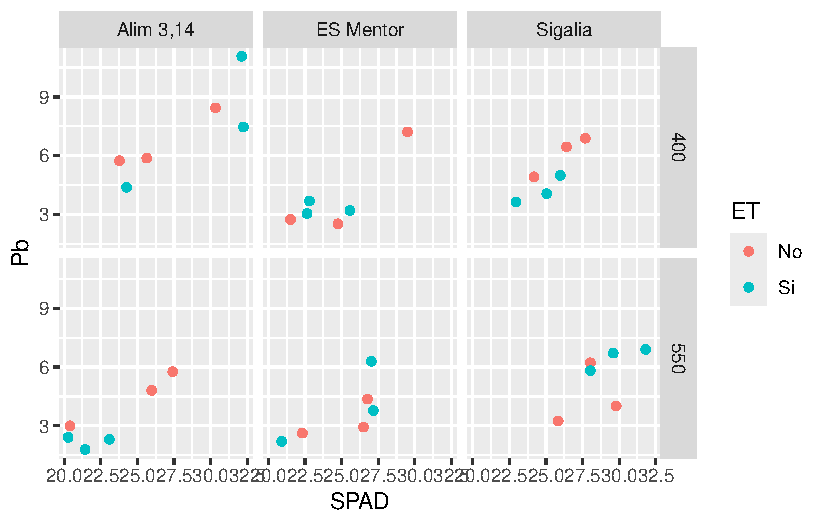
\includegraphics{curso_R_2025_q_files/figure-pdf/unnamed-chunk-89-3.pdf}

}

\end{figure}

\hypertarget{multifaceting}{%
\subsubsection{Multifaceting}\label{multifaceting}}

Si quisiéramos definir más de un nivel de división, podemos utilizar la
función \texttt{facet\_nested} del paquete \emph{ggh4x}. Por ejemplo de
la siguiente manera:

\begin{Shaded}
\begin{Highlighting}[]
\FunctionTok{library}\NormalTok{(ggh4x)}
\end{Highlighting}
\end{Shaded}

\begin{verbatim}
Warning: package 'ggh4x' was built under R version 4.4.2
\end{verbatim}

\begin{Shaded}
\begin{Highlighting}[]
\NormalTok{G2 }\SpecialCharTok{+} \FunctionTok{facet\_nested}\NormalTok{(.}\SpecialCharTok{\textasciitilde{}}\NormalTok{GT}\SpecialCharTok{+}\NormalTok{CO2) }\CommentTok{\# cada nivel de GT se divide por CO2}
\end{Highlighting}
\end{Shaded}

\begin{figure}[H]

{\centering 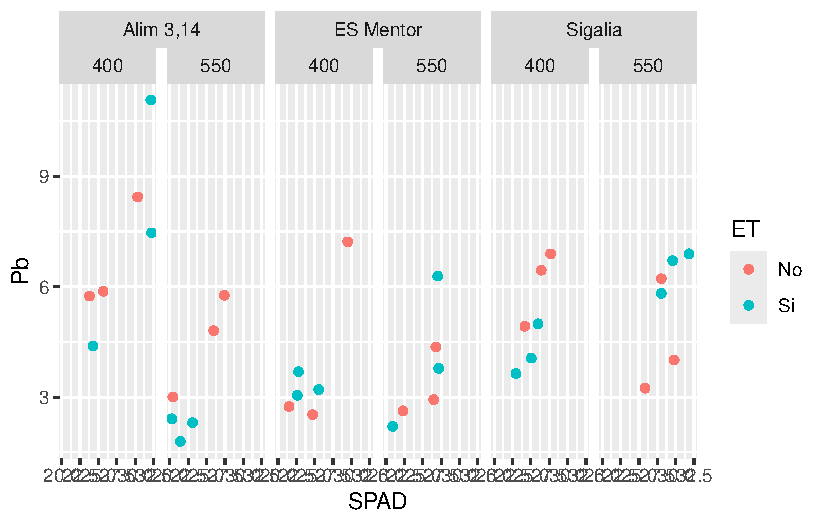
\includegraphics{curso_R_2025_q_files/figure-pdf/unnamed-chunk-90-1.pdf}

}

\end{figure}

\hypertarget{definiendo-la-estuxe9tica-de-nuestros-gruxe1ficos}{%
\subsection{Definiendo la estética de nuestros
gráficos}\label{definiendo-la-estuxe9tica-de-nuestros-gruxe1ficos}}

\hypertarget{exportaciuxf3n-y-ediciuxf3n-posterior-un-arma-de-doble-filo}{%
\subsubsection{Exportación y edición posterior: un arma de doble
filo}\label{exportaciuxf3n-y-ediciuxf3n-posterior-un-arma-de-doble-filo}}

La posibilidad de exportar un gráfico y editarlo posteriormente en otro
software siempre está sobre la mesa. Este apartado tiene como idea
presentar y analizar brevemente sus ventajas y desventajas.

En este caso la que más he utilizado y funciona muy bien es el uso de
imágenes vectorizadas. Si exportamos un archivo en formato svg, el mismo
podrá verse en esta forma en software de edición de imagen. El que yo
recomiendo es Inkscape, ya que es gratuito y multiplataforma y su forma
de uso es muy intuitivo. La ventaja de tener la imagen vectorizada es
que no perdemos calidad y además nos brinda la posibilidad de manipular
cada uno de los elementos del gráfico individualmente.

El manejo externo de los gráficos es una herramienta muy poderosa en
cuanto a las posibilidades que nos ofrece, ya que podemos modificar lo
que queramos a nuestro antojo y con muy buenos resultados. Sin embargo,
tiene una desventaja enorme: nuestra edición no es repetible. Esto
quiere decir, que si por algún motivo tuvimos que hacer el gráfico de
nuevo, todo el trabajo de edición empieza de cero. Y, al menos en mi
experiencia de trabajo, rehacer un gráfico ya hecho es cosa de todos los
días (decidimos incluir o no un outlier, corregimos datos, modificamos
un factor, cambiamos de idioma el gráfico, etc.).

Por estos motivos, mi recomendación es intentar hacer lo más posible
directamente en R y solo en casos de extrema necesidad acudir al
software externo. A pesar de esto, no deja de ser una herramienta
potente y a tener en cuenta.

\hypertarget{definiendo-el-theme-en-ggplot2}{%
\subsubsection{\texorpdfstring{Definiendo el \texttt{theme} en
ggplot2}{Definiendo el theme en ggplot2}}\label{definiendo-el-theme-en-ggplot2}}

Cuando realizamos un gráfico con \texttt{ggplot} la mayor parte de las
cuestiones estéticas se definen dentro del parámetro \texttt{theme}.
Este apartado nos permite modificar las letras del gráficos en general,
de los ejes, de los títulos de los ejes, la posición y estructura de la
leyenda, etc. La estructura general consiste en nombrar el elemento a
modificar, luego establecer el tipo de elemento, y finalmente modificar
los parámetros. Supongamos a modo de ejemplo que queremos que las
etiquetas del eje \emph{x} estén en negro, con tamaño de letra 12, con
inclinación vertical. Entonces escribiremos:

\begin{Shaded}
\begin{Highlighting}[]
\NormalTok{Gráfico }\SpecialCharTok{+}
  \FunctionTok{theme}\NormalTok{(}\AttributeTok{axis.text.x =} \FunctionTok{element\_text}\NormalTok{(}\AttributeTok{size=}\DecValTok{12}\NormalTok{ ,}
                                   \AttributeTok{colour =} \StringTok{"black"}\NormalTok{,}
                                   \AttributeTok{angle=} \DecValTok{90}\NormalTok{))}
\end{Highlighting}
\end{Shaded}

Podemos ir separando por comas diferentes elementos que queramos
modificar. Otra opción interesante es crear un objeto con todas nuestras
modificaciones, que luego podemos aplicar a todos nuestros gráficos.
También existen temas prediseñados que modifican varios parámetros a la
vez. Estos se introducen con el comando theme\_ donde las opciones son
muchas, en particular a mí me gusta la opción \texttt{theme\_pubr}
\footnote{Para más información del paquete \emph{ggpubr} dirigirse a
  https://rpkgs.datanovia.com/ggpubr/ . Es un paquete muy interesante
  orientado a publicaciones usando ggplot2.} del paquete \emph{ggpubr}.
Podemos combinar todo en un objeto, por ejemplo:

\begin{Shaded}
\begin{Highlighting}[]
\FunctionTok{library}\NormalTok{(ggpubr)}
\end{Highlighting}
\end{Shaded}

\begin{verbatim}

Adjuntando el paquete: 'ggpubr'
\end{verbatim}

\begin{verbatim}
The following object is masked from 'package:plyr':

    mutate
\end{verbatim}

\begin{Shaded}
\begin{Highlighting}[]
\NormalTok{THEME }\OtherTok{\textless{}{-}}\FunctionTok{theme\_pubr}\NormalTok{() }\SpecialCharTok{+}
\FunctionTok{theme}\NormalTok{(}\AttributeTok{plot.caption =} \FunctionTok{element\_text}\NormalTok{(}\AttributeTok{hjust =} \DecValTok{0}\NormalTok{, }\AttributeTok{vjust=}\NormalTok{.}\DecValTok{5}\NormalTok{),}
               \AttributeTok{plot.title.position =} \StringTok{"plot"}\NormalTok{,}
               \AttributeTok{plot.title =} \FunctionTok{element\_text}\NormalTok{(}\AttributeTok{size=}\FunctionTok{rel}\NormalTok{(}\FloatTok{1.5}\NormalTok{)),}
               \AttributeTok{text =} \FunctionTok{element\_text}\NormalTok{(}\AttributeTok{size=}\DecValTok{12}\NormalTok{, }\AttributeTok{colour =} \StringTok{"black"}\NormalTok{),}
               \AttributeTok{axis.text =} \FunctionTok{element\_text}\NormalTok{(}\AttributeTok{size=}\DecValTok{12}\NormalTok{ , }\AttributeTok{colour =} \StringTok{"black"}\NormalTok{),}
               \AttributeTok{axis.line =} \FunctionTok{element\_line}\NormalTok{(}\AttributeTok{colour =} \StringTok{"black"}\NormalTok{),}
               \AttributeTok{legend.position =} \StringTok{"right"}\NormalTok{,}
               \AttributeTok{legend.text =} \FunctionTok{element\_text}\NormalTok{(}\AttributeTok{size=}\DecValTok{12}\NormalTok{, }\AttributeTok{colour =} \StringTok{"black"}\NormalTok{),}
               \AttributeTok{legend.background =} \FunctionTok{element\_rect}\NormalTok{(}\AttributeTok{colour =} \StringTok{"black"}\NormalTok{)) }\CommentTok{\# recuadro de la leyenda}
\end{Highlighting}
\end{Shaded}

Luego podemos incorporarlo al final de los gráficos, así:

\begin{Shaded}
\begin{Highlighting}[]
\NormalTok{G1 }\SpecialCharTok{+}\NormalTok{ THEME}
\end{Highlighting}
\end{Shaded}

\begin{figure}[H]

{\centering 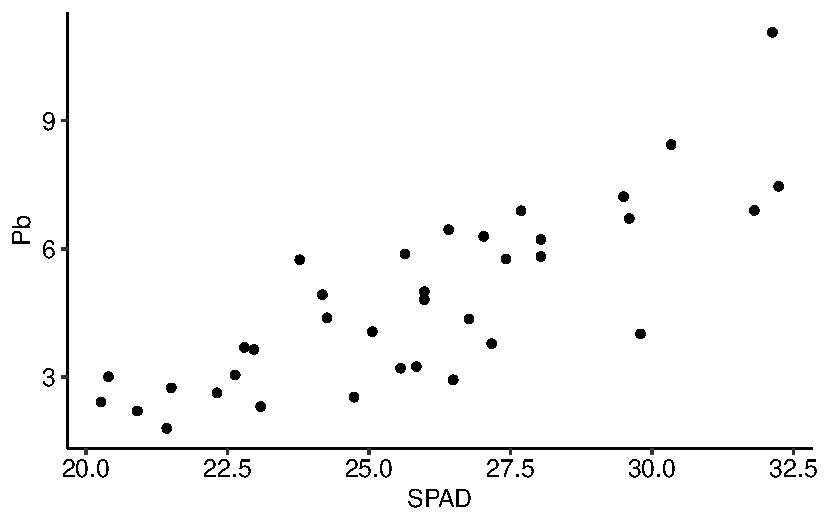
\includegraphics{curso_R_2025_q_files/figure-pdf/unnamed-chunk-93-1.pdf}

}

\end{figure}

\begin{Shaded}
\begin{Highlighting}[]
\NormalTok{G3 }\SpecialCharTok{+}\NormalTok{ THEME}
\end{Highlighting}
\end{Shaded}

\begin{figure}[H]

{\centering 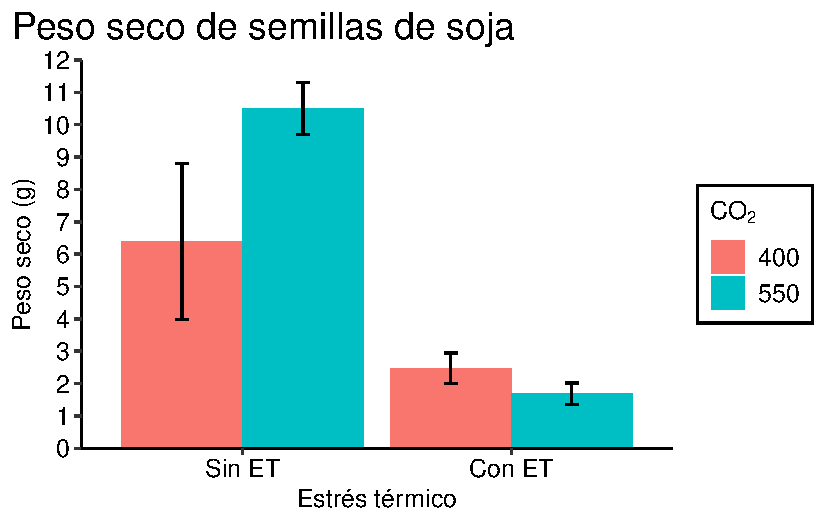
\includegraphics{curso_R_2025_q_files/figure-pdf/unnamed-chunk-93-2.pdf}

}

\end{figure}

\hypertarget{fuentes}{%
\subsubsection{Fuentes}\label{fuentes}}

Dentro de la opción \emph{text}, podemos elegir la fuente de nuestro
gráfico.

\begin{Shaded}
\begin{Highlighting}[]
\FunctionTok{...theme}\NormalTok{(}
    \AttributeTok{text =} \FunctionTok{element\_text}\NormalTok{(}\AttributeTok{family =} \StringTok{"Times New Roman"}\NormalTok{))}
\end{Highlighting}
\end{Shaded}

Las fuentes disponibles en windows no son muchas: ``Arial'', ``Times New
Roman'', ``Calibri'', ``Courier New'', ``Verdana''. Varían un poco de
acuerdo a nuestro sistema operativo. Con el paquete \emph{extrafont}
podemos incorporar bastantes más.

Para chequear las fuentes disponibles en windows ejecutamos:

\begin{Shaded}
\begin{Highlighting}[]
\FunctionTok{names}\NormalTok{(grDevices}\SpecialCharTok{::}\FunctionTok{windowsFonts}\NormalTok{())}
\end{Highlighting}
\end{Shaded}

\begin{verbatim}
[1] "serif" "sans"  "mono" 
\end{verbatim}

Para agregar en R las que tengamos en nuestro sistema podemos correr
\textbf{font\_import()}, luego cargarlas con \emph{loadfonts()} y ver la
lista con \emph{fonts()} :

\begin{Shaded}
\begin{Highlighting}[]
\FunctionTok{library}\NormalTok{(extrafont)}
\FunctionTok{loadfonts}\NormalTok{()}
\FunctionTok{fonts}\NormalTok{()}
\end{Highlighting}
\end{Shaded}

Algo muy importante, es que al momento de exportar como pdf nuestras
imágenes, la fuentes tienen que estar embebidas para que las pueda leer
cualquier lector de archivos pdf. Por suerte las nuevas versiones de
\emph{ggsave()} incluyen una opción que realiza esto de manera muy
simple:

\begin{Shaded}
\begin{Highlighting}[]
\NormalTok{G3 }\SpecialCharTok{+}
  \FunctionTok{theme}\NormalTok{(}\AttributeTok{text =} \FunctionTok{element\_text}\NormalTok{(}\AttributeTok{family =} \StringTok{"serif"}\NormalTok{, }\AttributeTok{size =} \DecValTok{18}\NormalTok{))}
\end{Highlighting}
\end{Shaded}

\begin{figure}[H]

{\centering 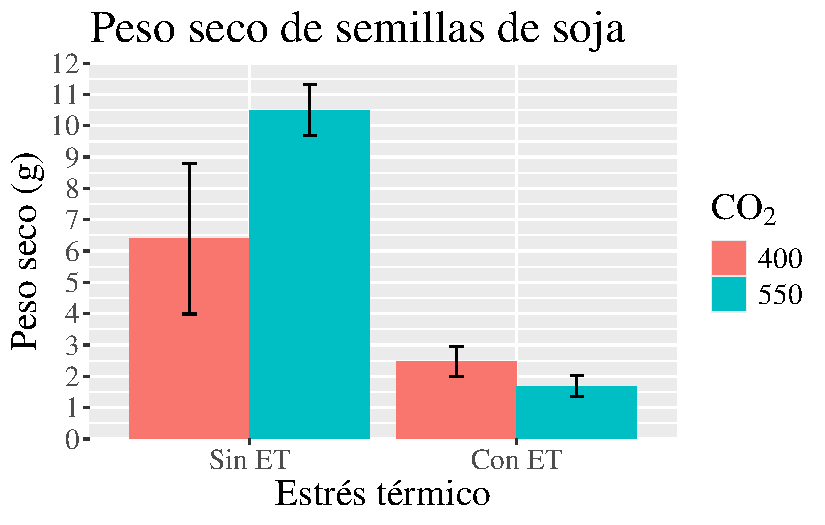
\includegraphics{curso_R_2025_q_files/figure-pdf/unnamed-chunk-97-1.pdf}

}

\end{figure}

\begin{Shaded}
\begin{Highlighting}[]
\NormalTok{G3 }\SpecialCharTok{+}
  \FunctionTok{theme}\NormalTok{(}\AttributeTok{text =} \FunctionTok{element\_text}\NormalTok{(}\AttributeTok{family =} \StringTok{"mono"}\NormalTok{, }\AttributeTok{size =} \DecValTok{18}\NormalTok{))}
\end{Highlighting}
\end{Shaded}

\begin{figure}[H]

{\centering 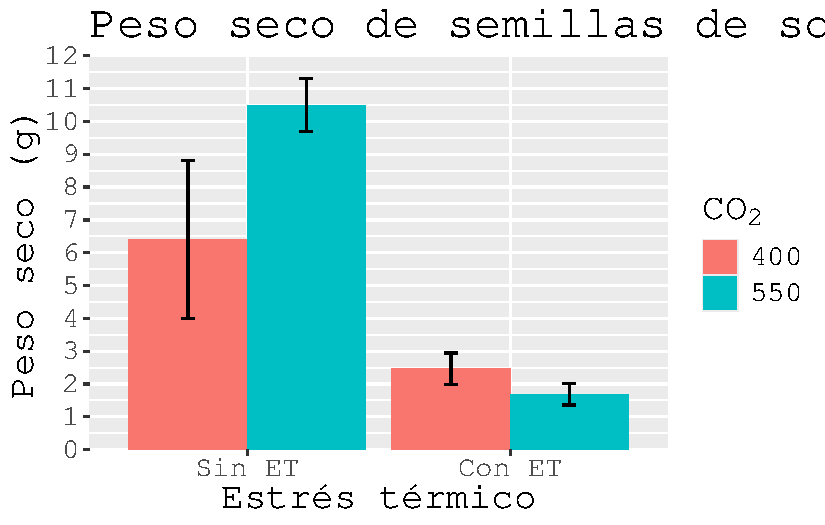
\includegraphics{curso_R_2025_q_files/figure-pdf/unnamed-chunk-97-2.pdf}

}

\end{figure}

\begin{Shaded}
\begin{Highlighting}[]
\FunctionTok{ggsave}\NormalTok{(}\StringTok{"G3.pdf"}\NormalTok{, }\AttributeTok{device =}\NormalTok{ cairo\_pdf)}
\end{Highlighting}
\end{Shaded}

\hypertarget{divisiuxf3n-de-la-ventana-gruxe1fica}{%
\subsection{División de la ventana
gráfica}\label{divisiuxf3n-de-la-ventana-gruxe1fica}}

Esta es una herramienta muy útil que nos permite visualizar más de un
gráfico a la vez en la ventana 4 de RStudio. Ya que esta ventana suele
ser pequeña, es recomendable marcar en \emph{Zoom} una vez creado el
conjunto de gráficos para verlo externamente.

\hypertarget{layout}{%
\subsubsection{layout}\label{layout}}

Esta opción ya la vimos anteriormente para los gráficos de supuestos.
Básicamente se debe especificar una matriz mediante el comando
\texttt{matrix} cuya estructura básica es:

\begin{Shaded}
\begin{Highlighting}[]
\FunctionTok{matrix}\NormalTok{(}\DecValTok{1}\SpecialCharTok{:}\NormalTok{n, }\CommentTok{\#cantidad de casilleros}
\NormalTok{       r,p) }\CommentTok{\# distribución en filas y columnas}
\end{Highlighting}
\end{Shaded}

Entonces para una matriz 2*2 será:

\begin{Shaded}
\begin{Highlighting}[]
\FunctionTok{matrix}\NormalTok{(}\DecValTok{1}\SpecialCharTok{:}\DecValTok{4}\NormalTok{,}\DecValTok{2}\NormalTok{,}\DecValTok{2}\NormalTok{)}
\end{Highlighting}
\end{Shaded}

Para una 3*4 será:

\begin{Shaded}
\begin{Highlighting}[]
\FunctionTok{matrix}\NormalTok{(}\DecValTok{1}\SpecialCharTok{:}\DecValTok{12}\NormalTok{,}\DecValTok{3}\NormalTok{,}\DecValTok{4}\NormalTok{)}
\end{Highlighting}
\end{Shaded}

Por lo tanto, el comando de división gráfica tendrá la forma:

\begin{Shaded}
\begin{Highlighting}[]
\FunctionTok{layout}\NormalTok{(}\FunctionTok{matrix}\NormalTok{(}\DecValTok{1}\SpecialCharTok{:}\DecValTok{2}\NormalTok{,}\DecValTok{2}\NormalTok{,}\DecValTok{1}\NormalTok{))}
\NormalTok{Gráfico }\DecValTok{1}
\NormalTok{Gráfico }\DecValTok{2}
\FunctionTok{layout}\NormalTok{(}\DecValTok{1}\NormalTok{) }\CommentTok{\# al cerrar volvemos a establecer una ventana única}
\end{Highlighting}
\end{Shaded}

Se deben incluir tantos gráficos como particiones creadas. Por ejemplo
viendo dos gráficos creados anteriormente:

\begin{Shaded}
\begin{Highlighting}[]
\CommentTok{\# 1 fila y 2 columnas}
\FunctionTok{layout}\NormalTok{(}\FunctionTok{matrix}\NormalTok{(}\DecValTok{1}\SpecialCharTok{:}\DecValTok{2}\NormalTok{,}\DecValTok{1}\NormalTok{,}\DecValTok{2}\NormalTok{))}
\FunctionTok{lineplot.CI}\NormalTok{(}\AttributeTok{x.factor =}\NormalTok{ SPAD, }\AttributeTok{response =}\NormalTok{ Pb, }\AttributeTok{data =}\NormalTok{ HOJA)}
\FunctionTok{boxplot}\NormalTok{(PS}\SpecialCharTok{\textasciitilde{}}\NormalTok{ET, }\AttributeTok{ylim =} \FunctionTok{c}\NormalTok{(}\DecValTok{0}\NormalTok{,}\DecValTok{12}\NormalTok{),  }\AttributeTok{data =}\NormalTok{ SEM\_Alim)}
\end{Highlighting}
\end{Shaded}

\begin{figure}[H]

{\centering 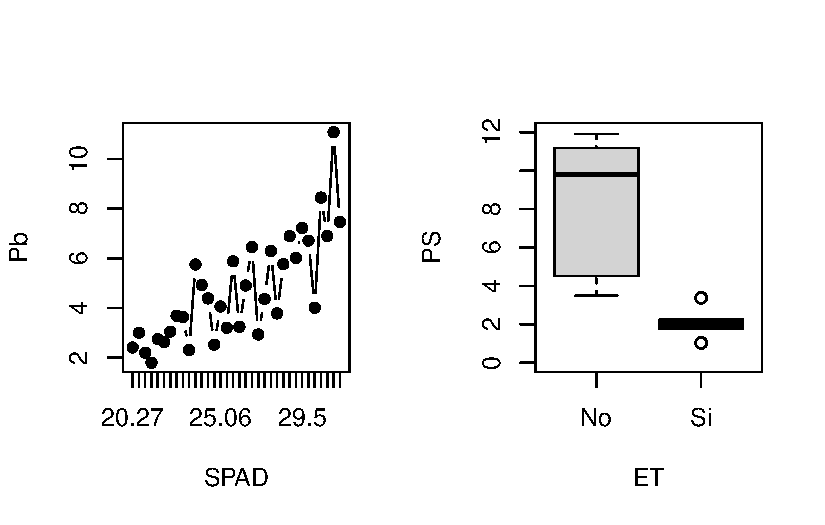
\includegraphics{curso_R_2025_q_files/figure-pdf/unnamed-chunk-103-1.pdf}

}

\end{figure}

\begin{Shaded}
\begin{Highlighting}[]
\FunctionTok{layout}\NormalTok{(}\DecValTok{1}\NormalTok{)}
\end{Highlighting}
\end{Shaded}

Los parámetros \texttt{widths} y \texttt{heights} permite establecer uno
más grande que el otro:

\begin{Shaded}
\begin{Highlighting}[]
\FunctionTok{layout}\NormalTok{(}\FunctionTok{matrix}\NormalTok{(}\DecValTok{1}\SpecialCharTok{:}\DecValTok{2}\NormalTok{,}\DecValTok{1}\NormalTok{,}\DecValTok{2}\NormalTok{), }\AttributeTok{widths =} \FunctionTok{c}\NormalTok{(}\DecValTok{2}\NormalTok{,}\DecValTok{1}\NormalTok{))}
\FunctionTok{lineplot.CI}\NormalTok{(}\AttributeTok{x.factor =}\NormalTok{ SPAD, }\AttributeTok{response =}\NormalTok{ Pb, }\AttributeTok{data =}\NormalTok{ HOJA)}
\FunctionTok{boxplot}\NormalTok{(PS}\SpecialCharTok{\textasciitilde{}}\NormalTok{ET, }\AttributeTok{ylim =} \FunctionTok{c}\NormalTok{(}\DecValTok{0}\NormalTok{,}\DecValTok{12}\NormalTok{),  }\AttributeTok{data =}\NormalTok{ SEM\_Alim)}
\end{Highlighting}
\end{Shaded}

\begin{figure}[H]

{\centering 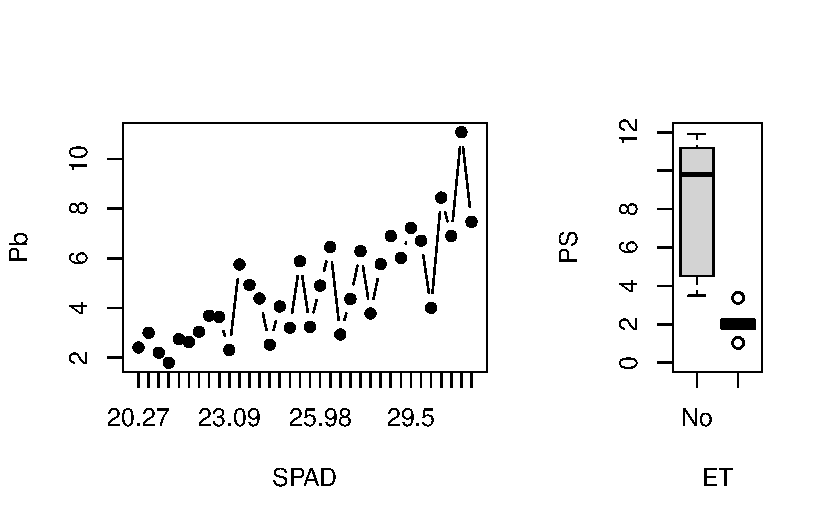
\includegraphics{curso_R_2025_q_files/figure-pdf/unnamed-chunk-104-1.pdf}

}

\end{figure}

\begin{Shaded}
\begin{Highlighting}[]
\FunctionTok{layout}\NormalTok{(}\DecValTok{1}\NormalTok{)}
\end{Highlighting}
\end{Shaded}

\hypertarget{par}{%
\subsubsection{par}\label{par}}

La función \texttt{par} también nos permite dividir la ventana gráfica.
Las opciones que ofrece son muchísimas, incluyendo opciones avanzadas
del manejo de márgenes. Aquí solo la nombraremos brevemente, para
obtener el mismo resultado mostrado anteriormente podemos hacer:

\begin{Shaded}
\begin{Highlighting}[]
\FunctionTok{par}\NormalTok{(}\AttributeTok{mfrow =} \FunctionTok{c}\NormalTok{(}\DecValTok{1}\NormalTok{, }\DecValTok{2}\NormalTok{)) }\CommentTok{\# filas y columnas}
\FunctionTok{lineplot.CI}\NormalTok{(}\AttributeTok{x.factor =}\NormalTok{ SPAD, }\AttributeTok{response =}\NormalTok{ Pb, }\AttributeTok{data =}\NormalTok{ HOJA)}
\FunctionTok{boxplot}\NormalTok{(PS}\SpecialCharTok{\textasciitilde{}}\NormalTok{ET, }\AttributeTok{ylim =} \FunctionTok{c}\NormalTok{(}\DecValTok{0}\NormalTok{,}\DecValTok{12}\NormalTok{),  }\AttributeTok{data =}\NormalTok{ SEM\_Alim)}
\FunctionTok{par}\NormalTok{(}\AttributeTok{mfrow =} \FunctionTok{c}\NormalTok{(}\DecValTok{1}\NormalTok{, }\DecValTok{1}\NormalTok{)) }\CommentTok{\# volvemos a como estaba antes}
\end{Highlighting}
\end{Shaded}

Tanto la función \texttt{layout} como \texttt{par} son compatibles con
\emph{Devices} para la exportación.

\hypertarget{grid.arrange}{%
\subsubsection{grid.arrange}\label{grid.arrange}}

Esta función se encuentra dentro del paquete \textbf{gridExtra} y nos
permite subdividir la ventana gráfica en un entorno de ggplot2. Además,
es enteramente compatible con \texttt{ggsave} para su exportación.

Su estructura general tiene la forma:

\begin{Shaded}
\begin{Highlighting}[]
\FunctionTok{grid.arrange}\NormalTok{(}
\NormalTok{  Grafico1 }\SpecialCharTok{+}\NormalTok{ modificaciones,}
\NormalTok{  Grafico2 }\SpecialCharTok{+}\NormalTok{ modificaciones,}
\NormalTok{  .....,}
  \AttributeTok{ncol=}\NormalTok{ número de columnas,}
  \AttributeTok{nrow=}\NormalTok{ número de filas,  }\CommentTok{\# en general con establecer el número de columnas es suficiente}
  \AttributeTok{widths=}\FunctionTok{c}\NormalTok{(}\DecValTok{1}\NormalTok{,}\DecValTok{1}\NormalTok{,}\DecValTok{2}\NormalTok{), }\CommentTok{\# podemos modificar el ancho relativo de cada columna}
  \AttributeTok{heights=}\FunctionTok{c}\NormalTok{(}\DecValTok{3}\NormalTok{,}\DecValTok{4}\NormalTok{,}\DecValTok{4}\NormalTok{) }\CommentTok{\# lo mismo para las filas}
\NormalTok{)}
\end{Highlighting}
\end{Shaded}

Como los gráficos en ggplot suelen involucrar muchas líneas, es
conveniente crear un objeto con cada gráfico a utilizar. Por ejemplo,
podemos combinar los gráficos creados anteriormente:

\begin{Shaded}
\begin{Highlighting}[]
\FunctionTok{grid.arrange}\NormalTok{(G2, G3, }\AttributeTok{ncol=}\DecValTok{2}\NormalTok{)}
\end{Highlighting}
\end{Shaded}

\begin{figure}[H]

{\centering 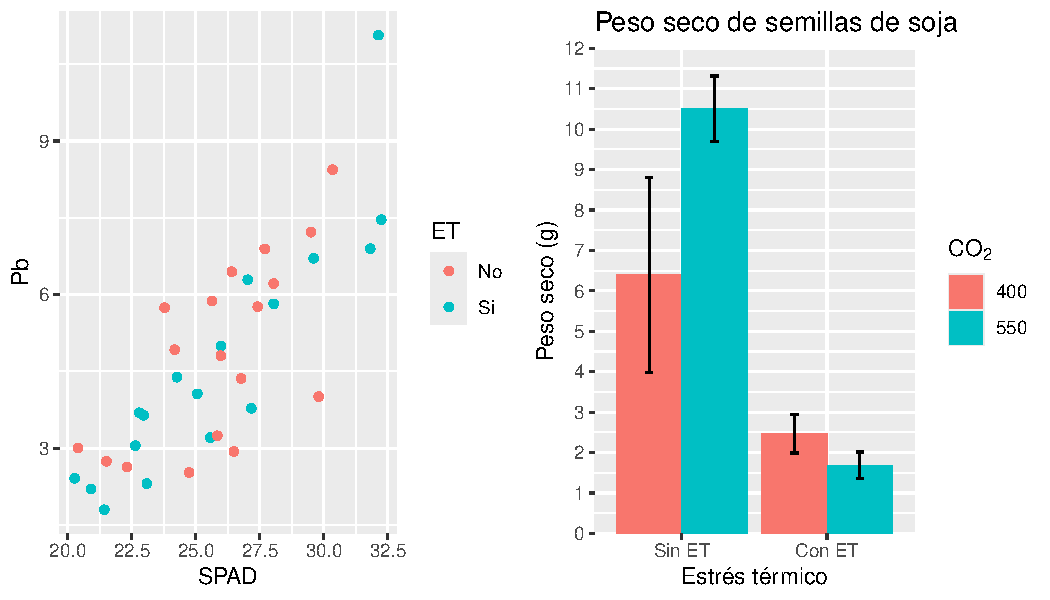
\includegraphics{curso_R_2025_q_files/figure-pdf/unnamed-chunk-107-1.pdf}

}

\end{figure}

Para exportar estos gráficos, hay que reemplazar en el mismo comando
\texttt{ggsave} por todo el arreglo con \texttt{grid.arrange}.

\hypertarget{patchwork}{%
\subsubsection{patchwork}\label{patchwork}}

El paquete \textbf{patchwork}\footnote{Para más información acerca del
  uso de \textbf{patchwork} recomiendo la página
  https://patchwork.data-imaginist.com/index.html.} permite una opción
muy versátil para la combinación de gráficos y división de la ventana
gráfica. Su uso además es muy sencillo, ya que si ya creamos los
gráficos y tenemos el paquete cargado, podemos unir gráficos simplemente
sumándolos:

\begin{Shaded}
\begin{Highlighting}[]
\NormalTok{G2 }\SpecialCharTok{+}\NormalTok{ G3}
\end{Highlighting}
\end{Shaded}

\begin{figure}[H]

{\centering 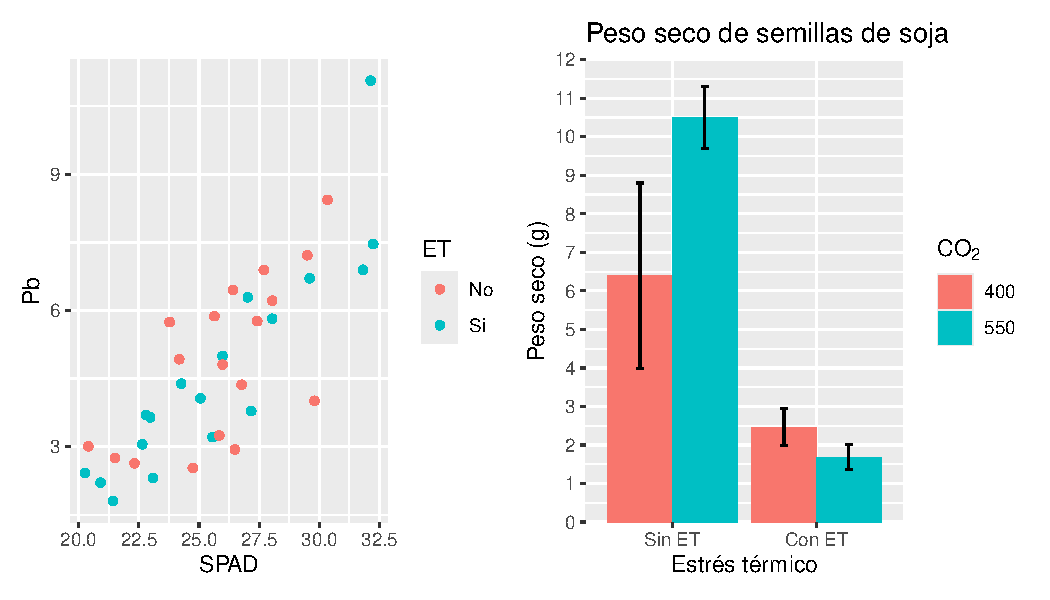
\includegraphics{curso_R_2025_q_files/figure-pdf/unnamed-chunk-108-1.pdf}

}

\end{figure}

Existen diferentes combinaciones posibles, por ejemplo:

\begin{Shaded}
\begin{Highlighting}[]
\NormalTok{(G2 }\SpecialCharTok{+}\NormalTok{ G3)}\SpecialCharTok{/}\NormalTok{ G1}
\end{Highlighting}
\end{Shaded}

\begin{figure}[H]

{\centering 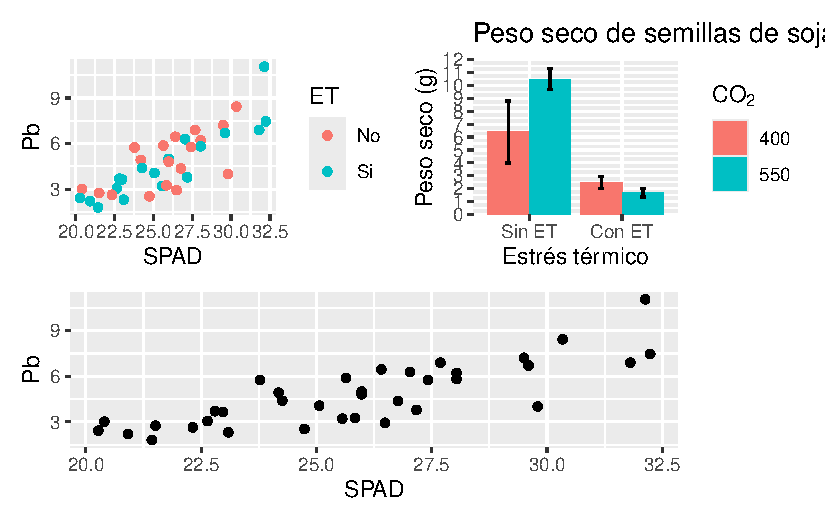
\includegraphics{curso_R_2025_q_files/figure-pdf/unnamed-chunk-109-1.pdf}

}

\end{figure}

Dentro de este paquete se encuentra la función \texttt{wrap\_plots} que
acomoda correctamente los gráficos y alinea los ejes. Así podemos
correr:

\begin{Shaded}
\begin{Highlighting}[]
\FunctionTok{wrap\_plots}\NormalTok{(G1, G2, G3)}
\end{Highlighting}
\end{Shaded}

\begin{figure}[H]

{\centering 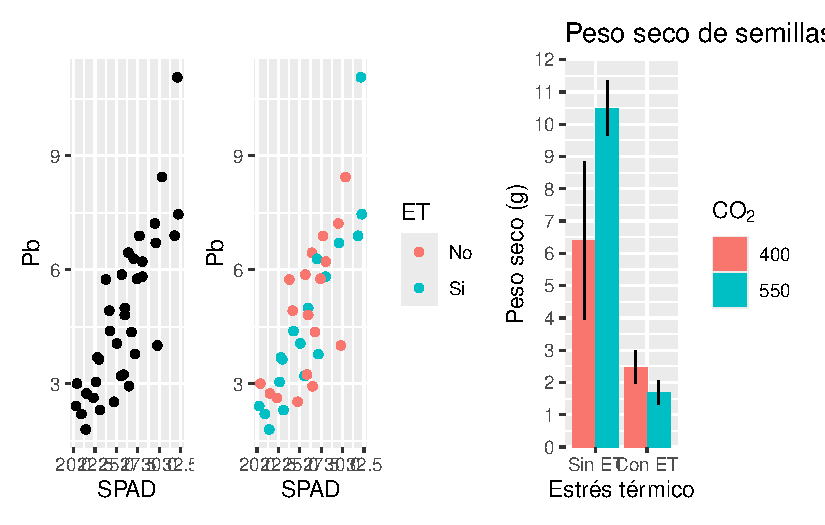
\includegraphics{curso_R_2025_q_files/figure-pdf/unnamed-chunk-110-1.pdf}

}

\end{figure}

Podemos modificar la estructura del gráfico con la función
\texttt{plot\_layout} dentro de \texttt{wrap\_plot}. Aquí podemos
definir la estructura de filas y columnas, la posición de las leyendas
(o agruparlas en algún sector). Por su parte, se pueden modificar e
incluso automatizar anotaciones con \texttt{plot\_annotation}. Por
ejemplo modificando el agrupamiento anterior:

\begin{Shaded}
\begin{Highlighting}[]
\FunctionTok{wrap\_plots}\NormalTok{(G1 }\SpecialCharTok{+}\NormalTok{ G2 }\SpecialCharTok{+}\NormalTok{ G3 }\SpecialCharTok{+}
             \FunctionTok{plot\_layout}\NormalTok{(}\AttributeTok{ncol =} \DecValTok{1}\NormalTok{,}
                         \AttributeTok{nrow =} \DecValTok{3}\NormalTok{,}
                         \AttributeTok{byrow =} \ConstantTok{NULL}\NormalTok{,}
                         \AttributeTok{guides =} \StringTok{\textquotesingle{}collect\textquotesingle{}}\NormalTok{)) }\SpecialCharTok{+} \CommentTok{\# muestra las leyendas juntas}
  \FunctionTok{plot\_annotation}\NormalTok{(}\AttributeTok{tag\_levels =} \StringTok{\textquotesingle{}a\textquotesingle{}}\NormalTok{, }\CommentTok{\# establecemos el tipo de enumeración}
                  \AttributeTok{tag\_prefix =} \StringTok{\textquotesingle{}(\textquotesingle{}}\NormalTok{,}
                  \AttributeTok{tag\_suffix =} \StringTok{\textquotesingle{})\textquotesingle{}}\NormalTok{)}
\end{Highlighting}
\end{Shaded}

\begin{figure}[H]

{\centering 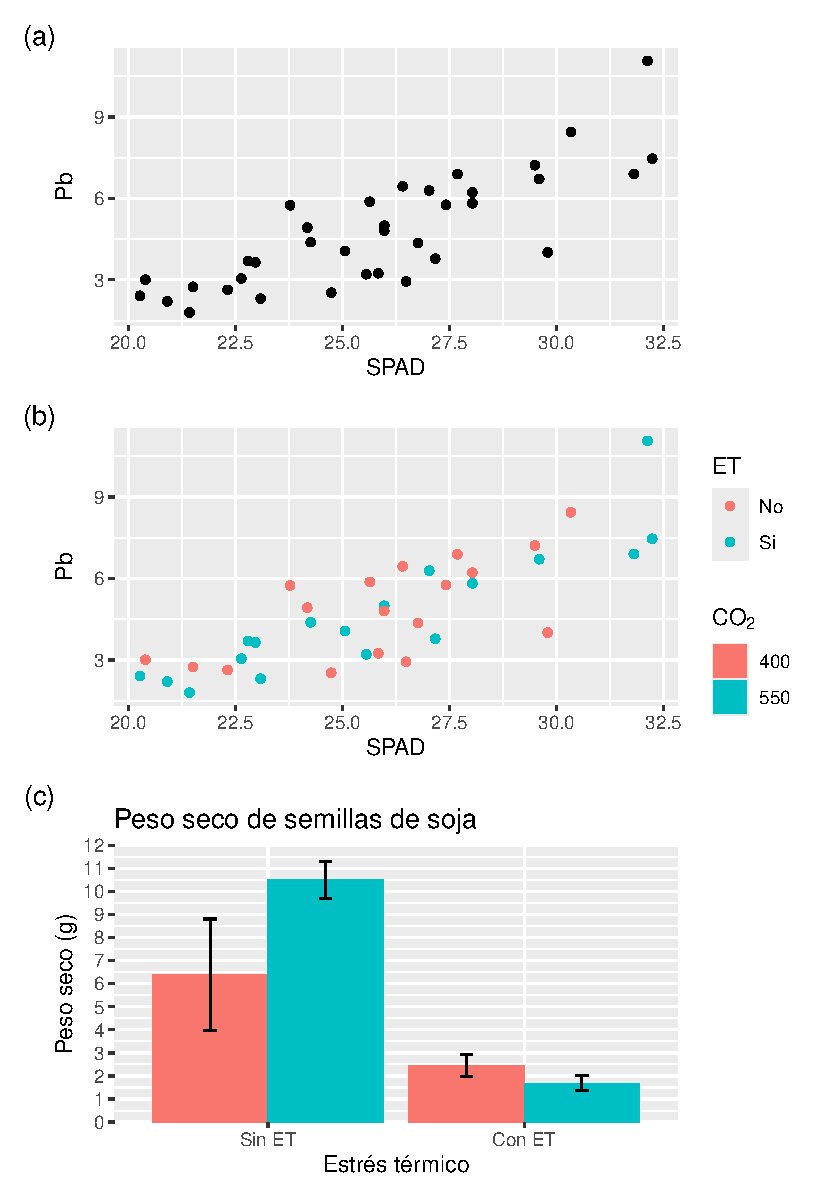
\includegraphics{curso_R_2025_q_files/figure-pdf/unnamed-chunk-111-1.pdf}

}

\end{figure}

Veremos más adelante algunas otras posibilidades con este paquete. Para
exportar los gráficos se procede de igual manera que con cualquier otro
gráfico de ggplot mediante la función \texttt{ggsave}.

También si los gráficos estuvieran combinados con \textbf{patchwork}
podemos incluir la cuestión estética a todos a la vez al final separando
con el comando \&:

\begin{Shaded}
\begin{Highlighting}[]
\FunctionTok{wrap\_plots}\NormalTok{(G1 }\SpecialCharTok{+}\NormalTok{ G2 }\SpecialCharTok{+}\NormalTok{ G3 }\SpecialCharTok{+}
             \FunctionTok{plot\_layout}\NormalTok{(}\AttributeTok{ncol =} \DecValTok{1}\NormalTok{,}
                         \AttributeTok{nrow =} \DecValTok{3}\NormalTok{,}
                         \AttributeTok{guides =} \StringTok{\textquotesingle{}collect\textquotesingle{}}\NormalTok{)) }\SpecialCharTok{+}
  \FunctionTok{plot\_annotation}\NormalTok{(}\AttributeTok{tag\_levels =} \StringTok{\textquotesingle{}a\textquotesingle{}}\NormalTok{,}
                  \AttributeTok{tag\_prefix =} \StringTok{\textquotesingle{}(\textquotesingle{}}\NormalTok{,}
                  \AttributeTok{tag\_suffix =} \StringTok{\textquotesingle{})\textquotesingle{}}\NormalTok{) }\SpecialCharTok{\&}
\NormalTok{  THEME}
\end{Highlighting}
\end{Shaded}

\begin{figure}[H]

{\centering 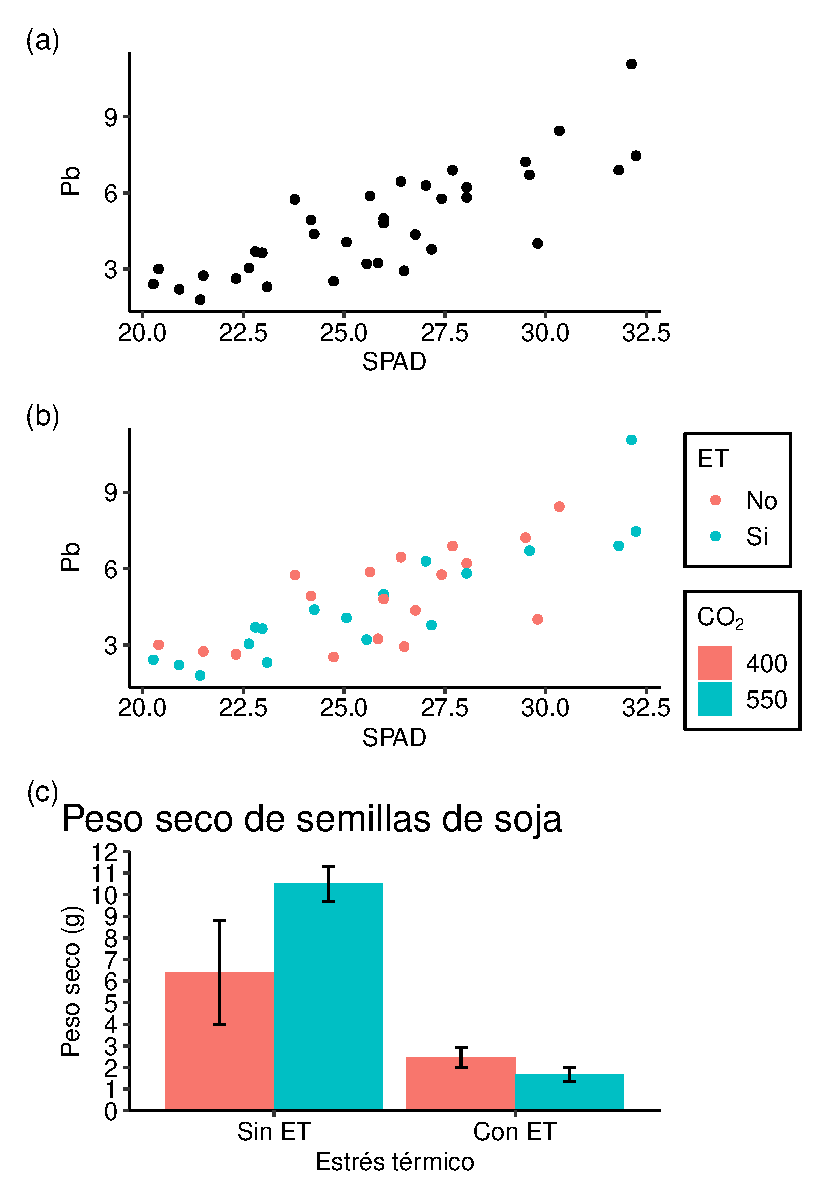
\includegraphics{curso_R_2025_q_files/figure-pdf/unnamed-chunk-112-1.pdf}

}

\end{figure}

Si dos de los gráficos comparten el eje x (por ejemplo), puede ser de
utilidad ocultar el título en uno de ellos, o incluso ocultar la escala
en el eje. Esto se puede hacer de diferentes maneras, pero aquí les
muestro una incluyendo el elemento vacío en el tema con
\emph{element\_blank} :

\begin{Shaded}
\begin{Highlighting}[]
\FunctionTok{wrap\_plots}\NormalTok{(G1 }\SpecialCharTok{+}\NormalTok{ THEME }\SpecialCharTok{+}
             \FunctionTok{theme}\NormalTok{(}\AttributeTok{axis.title.x =} \FunctionTok{element\_blank}\NormalTok{(),}
                      \AttributeTok{axis.text.x =} \FunctionTok{element\_blank}\NormalTok{())}\SpecialCharTok{+} 
\NormalTok{          G2 }\SpecialCharTok{+}\NormalTok{ THEME }\SpecialCharTok{+}
             \FunctionTok{plot\_layout}\NormalTok{(}\AttributeTok{ncol =} \DecValTok{1}\NormalTok{,}
                         \AttributeTok{nrow =} \DecValTok{2}\NormalTok{,}
                         \AttributeTok{guides =} \StringTok{\textquotesingle{}collect\textquotesingle{}}\NormalTok{)) }\SpecialCharTok{+}
  \FunctionTok{plot\_annotation}\NormalTok{(}\AttributeTok{tag\_levels =} \StringTok{\textquotesingle{}a\textquotesingle{}}\NormalTok{,}
                  \AttributeTok{tag\_prefix =} \StringTok{\textquotesingle{}(\textquotesingle{}}\NormalTok{,}
                  \AttributeTok{tag\_suffix =} \StringTok{\textquotesingle{})\textquotesingle{}}\NormalTok{)}
\end{Highlighting}
\end{Shaded}

\begin{figure}[H]

{\centering 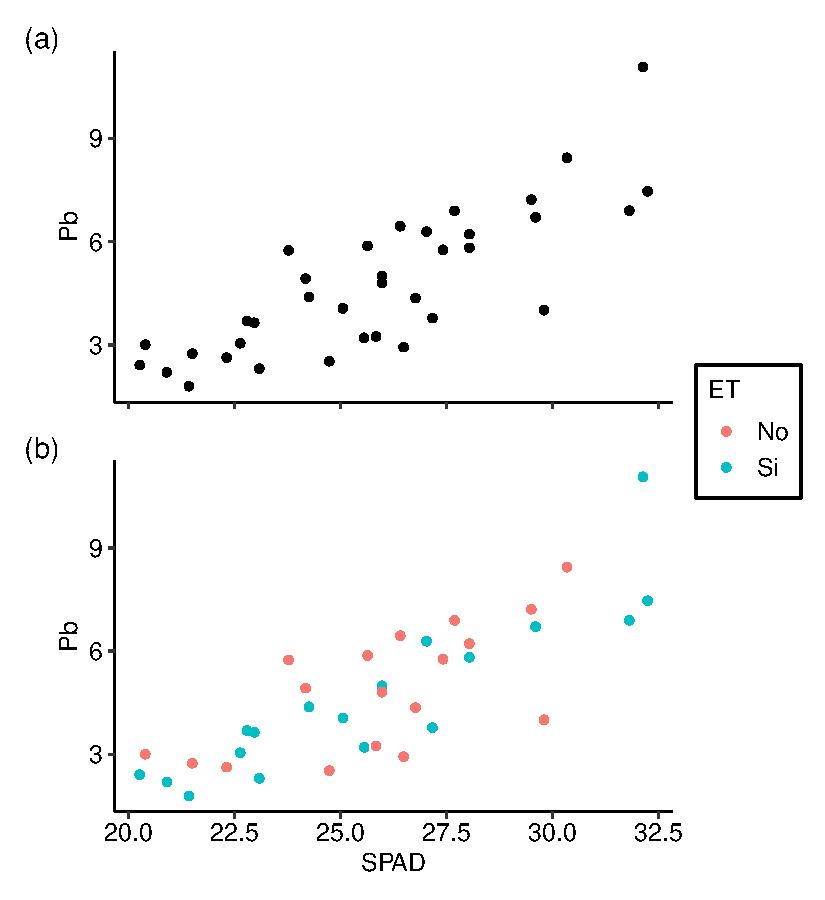
\includegraphics{curso_R_2025_q_files/figure-pdf/unnamed-chunk-113-1.pdf}

}

\end{figure}

\hypertarget{actividad-6}{%
\subsection{Actividad 6}\label{actividad-6}}

Exporte los dos gráficos que realizó en las actividades 3 y 5 combinados
en una sola figura de dos columnas y una fila, agregue etiquetas a cada
uno, aplique colores y escalas a los ejes. Junte las leyendas en una
sola.

\href{../}{Volver al inicio}

\hypertarget{unidad-5.-otros-tipos-y-paruxe1metros-gruxe1ficos}{%
\section{Unidad 5. Otros tipos y parámetros
gráficos}\label{unidad-5.-otros-tipos-y-paruxe1metros-gruxe1ficos}}

\hypertarget{gruxe1ficos-de-uxe1rea}{%
\subsection{Gráficos de área}\label{gruxe1ficos-de-uxe1rea}}

Para trabajar en de aquí en adelante utilizaremos otra base de datos. La
misma la armé en base a los datos de superficie cultivada, producción y
rendimiento de soja en Argentina y el mundo (extraída de informes de la
FAO\footnote{FAOSTATS. https://www.fao.org/faostat/en/\#data/QCL}) desde
1960 hasta 2023.

\begin{Shaded}
\begin{Highlighting}[]
\NormalTok{soja }\OtherTok{\textless{}{-}} \FunctionTok{read\_csv}\NormalTok{(}\StringTok{"produccion\_soja\_2023.csv"}\NormalTok{)}

\CommentTok{\# Dividiremos la base de datos en dos}
\NormalTok{mundo }\OtherTok{\textless{}{-}}\NormalTok{ soja }\SpecialCharTok{\%\textgreater{}\%}
  \FunctionTok{filter}\NormalTok{(Area }\SpecialCharTok{==} \StringTok{"World"}\NormalTok{)}

\NormalTok{argentina }\OtherTok{\textless{}{-}}\NormalTok{ soja }\SpecialCharTok{\%\textgreater{}\%}
  \FunctionTok{filter}\NormalTok{(Area }\SpecialCharTok{==} \StringTok{"Argentina"}\NormalTok{)}
\end{Highlighting}
\end{Shaded}

En primer lugar introduciremos un nuevo geom: \texttt{geom\_area}. Como
su nombre lo indica, permite graficar superficies completas en base a
una escala continua. En este caso usaremos como eje \emph{x} los años,
como si fueran continuos. Así por ejemplo podemos graficar la variación
de la superficie cultivada a lo largo del tiempo:

\begin{Shaded}
\begin{Highlighting}[]
\FunctionTok{ggplot}\NormalTok{(argentina, }\FunctionTok{aes}\NormalTok{(Year, Sup}\SpecialCharTok{/}\DecValTok{1000000}\NormalTok{))}\SpecialCharTok{+} \CommentTok{\# editamos la sup para no ver números tan grandes}
  \FunctionTok{geom\_area}\NormalTok{(}\AttributeTok{fill=}\StringTok{"cornflowerblue"}\NormalTok{, }\AttributeTok{col=}\StringTok{"gray21"}\NormalTok{) }\SpecialCharTok{+}
  \FunctionTok{scale\_y\_continuous}\NormalTok{(}\AttributeTok{expand =} \FunctionTok{c}\NormalTok{(}\DecValTok{0}\NormalTok{,}\DecValTok{0}\NormalTok{), }\AttributeTok{breaks =} \FunctionTok{seq}\NormalTok{(}\DecValTok{0}\NormalTok{, }\DecValTok{25}\NormalTok{, }\AttributeTok{by =} \DecValTok{5}\NormalTok{))}\SpecialCharTok{+}
  \FunctionTok{scale\_x\_continuous}\NormalTok{(}\AttributeTok{expand =} \FunctionTok{c}\NormalTok{(}\DecValTok{0}\NormalTok{,}\DecValTok{0}\NormalTok{),}\AttributeTok{breaks =} \FunctionTok{seq}\NormalTok{(}\DecValTok{1960}\NormalTok{,}\DecValTok{2025}\NormalTok{, }\AttributeTok{by=}\DecValTok{5}\NormalTok{))}\SpecialCharTok{+}
  \FunctionTok{labs}\NormalTok{(}\AttributeTok{x=} \StringTok{"Años"}\NormalTok{,}
    \AttributeTok{y=} \StringTok{"Superficie sembrada [millones de ha]"}\NormalTok{) }\SpecialCharTok{+}
\NormalTok{  THEME}
\end{Highlighting}
\end{Shaded}

\begin{figure}[H]

{\centering 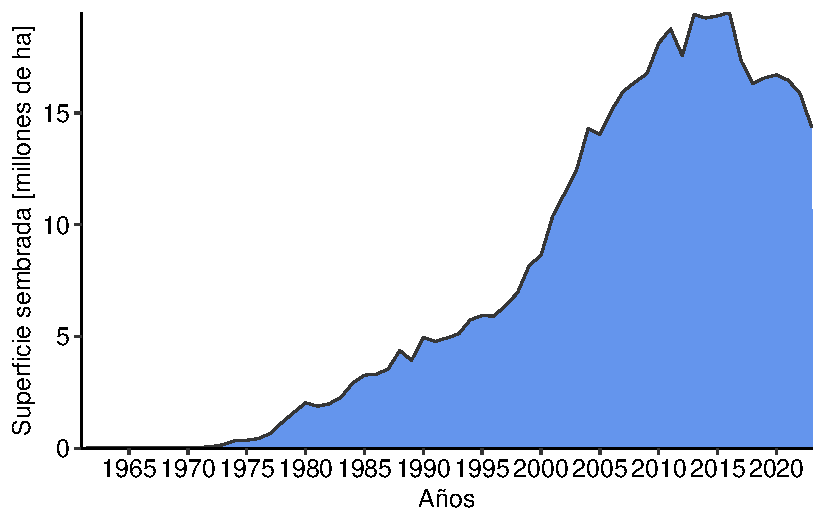
\includegraphics[width=1\textwidth,height=\textheight]{curso_R_2025_q_files/figure-pdf/unnamed-chunk-115-1.pdf}

}

\end{figure}

Ahora supongamos que queremos graficar al mismo tiempo la superficie de
Argentina y la global. Una opción sería dividir la variable Sup entre
las regiones por \emph{fill}.

\begin{Shaded}
\begin{Highlighting}[]
\FunctionTok{ggplot}\NormalTok{(soja, }\FunctionTok{aes}\NormalTok{(Year, Sup}\SpecialCharTok{/}\DecValTok{1000000}\NormalTok{, }\AttributeTok{fill=}\NormalTok{Area))}\SpecialCharTok{+}
  \FunctionTok{geom\_area}\NormalTok{(}\AttributeTok{col=}\StringTok{"gray21"}\NormalTok{) }\SpecialCharTok{+}
  \FunctionTok{scale\_y\_continuous}\NormalTok{(}\AttributeTok{expand =} \FunctionTok{c}\NormalTok{(}\DecValTok{0}\NormalTok{,}\DecValTok{0}\NormalTok{), }\AttributeTok{breaks =} \FunctionTok{seq}\NormalTok{(}\DecValTok{0}\NormalTok{, }\DecValTok{150}\NormalTok{, }\AttributeTok{by =} \DecValTok{10}\NormalTok{))}\SpecialCharTok{+}
  \FunctionTok{scale\_x\_continuous}\NormalTok{(}\AttributeTok{expand =} \FunctionTok{c}\NormalTok{(}\DecValTok{0}\NormalTok{,}\DecValTok{0}\NormalTok{),}\AttributeTok{breaks =} \FunctionTok{seq}\NormalTok{(}\DecValTok{1960}\NormalTok{,}\DecValTok{2025}\NormalTok{, }\AttributeTok{by=}\DecValTok{5}\NormalTok{))}\SpecialCharTok{+}
  \FunctionTok{labs}\NormalTok{(}\AttributeTok{x=} \StringTok{"Años"}\NormalTok{,}
    \AttributeTok{y=} \StringTok{"Superficie sembrada [millones de ha]"}\NormalTok{) }\SpecialCharTok{+}
\NormalTok{  THEME}
\end{Highlighting}
\end{Shaded}

\begin{figure}[H]

{\centering 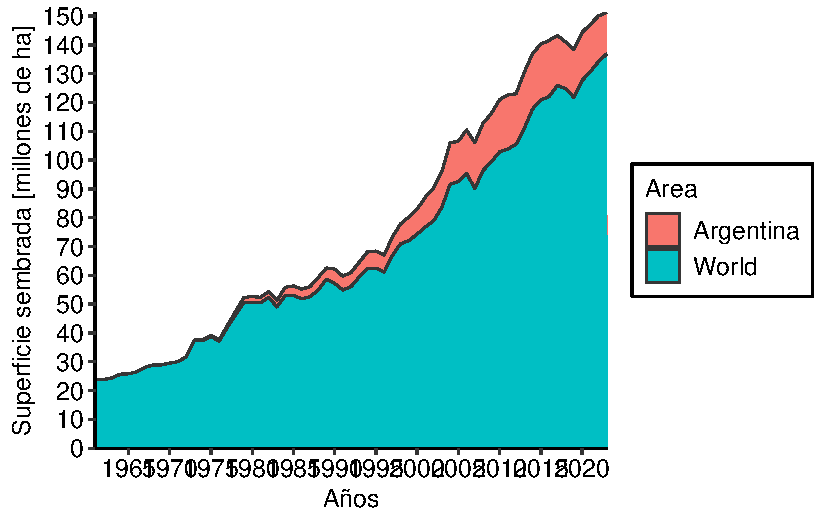
\includegraphics[width=1\textwidth,height=\textheight]{curso_R_2025_q_files/figure-pdf/unnamed-chunk-116-1.pdf}

}

\end{figure}

Si bien parece funcionar, al incluir esta opción geom\_area apila los
datos de una región con la otra. Por lo tanto, lo que vamos a hacer es
superponer dos gráficos de área al mismo tiempo. Para ello
introduciremos una nueva idea que es la de utilizar dos bases de datos
diferentes en el mismo gráfico. Cuando creamos nuestro gráfico
(ggplot(aes(\ldots))) los \emph{geom} que introduzcamos luego
``heredan'' tanto la base de datos como la estructura x-y determinada
por aes que acompaña a ggplot. Si nuestro nuevo \emph{geom} requiere una
diferente, debemos expresamente introducirla. Finalmente, como la
inclusión de nuevos \emph{geom} no incorpora una leyenda, con la función
\emph{annotate} podemos introducir texto en algún lugar específico para
clarificar qué significa cada área. También es posible introducir
segmentos, flechas y otros elementos con esta función. Veamos cómo
quedaría:

\begin{Shaded}
\begin{Highlighting}[]
\FunctionTok{ggplot}\NormalTok{(mundo, }\FunctionTok{aes}\NormalTok{(Year, Sup}\SpecialCharTok{/}\DecValTok{1000000}\NormalTok{))}\SpecialCharTok{+} \CommentTok{\# aes principal}
  \FunctionTok{geom\_area}\NormalTok{(}\AttributeTok{fill=}\StringTok{"burlywood3"}\NormalTok{, }\AttributeTok{col=}\StringTok{"gray21"}\NormalTok{) }\SpecialCharTok{+} \CommentTok{\# primer área, es la que va al fondo}
  \FunctionTok{scale\_y\_continuous}\NormalTok{(}\AttributeTok{expand =} \FunctionTok{c}\NormalTok{(}\DecValTok{0}\NormalTok{,}\DecValTok{0}\NormalTok{), }\AttributeTok{breaks =} \FunctionTok{seq}\NormalTok{(}\DecValTok{0}\NormalTok{,}\DecValTok{120}\NormalTok{, }\AttributeTok{by =} \DecValTok{10}\NormalTok{))}\SpecialCharTok{+}
  \FunctionTok{scale\_x\_continuous}\NormalTok{(}\AttributeTok{expand =} \FunctionTok{c}\NormalTok{(}\DecValTok{0}\NormalTok{,}\DecValTok{0}\NormalTok{),}\AttributeTok{breaks =} \FunctionTok{seq}\NormalTok{(}\DecValTok{1960}\NormalTok{,}\DecValTok{2025}\NormalTok{, }\AttributeTok{by=}\DecValTok{5}\NormalTok{))}\SpecialCharTok{+}
  \FunctionTok{labs}\NormalTok{(}\AttributeTok{x=} \StringTok{"Años"}\NormalTok{,}
       \AttributeTok{y=} \StringTok{"Superficie sembrada [millones de ha]"}\NormalTok{) }\SpecialCharTok{+}
  \FunctionTok{geom\_area}\NormalTok{(}\AttributeTok{data=}\NormalTok{ argentina, }\FunctionTok{aes}\NormalTok{(Year, Sup}\SpecialCharTok{/}\DecValTok{1000000}\NormalTok{), }\CommentTok{\# segunda, aparece al frente}
            \AttributeTok{fill=}\StringTok{"cornflowerblue"}\NormalTok{, }\AttributeTok{col=}\StringTok{"gray21"}\NormalTok{)}\SpecialCharTok{+}
  \FunctionTok{annotate}\NormalTok{(}\StringTok{"text"}\NormalTok{, }\AttributeTok{x=}\DecValTok{2008}\NormalTok{, }\AttributeTok{y=} \DecValTok{8}\NormalTok{, }\AttributeTok{label =} \StringTok{"Argentina"}\NormalTok{, }\CommentTok{\# agregamos texto en un lugar específico}
           \AttributeTok{size=}\DecValTok{6}\NormalTok{)}\SpecialCharTok{+}
  \FunctionTok{annotate}\NormalTok{(}\StringTok{"text"}\NormalTok{, }\AttributeTok{x=}\DecValTok{1990}\NormalTok{, }\AttributeTok{y=} \DecValTok{35}\NormalTok{, }\AttributeTok{label =} \StringTok{"Mundo"}\NormalTok{, }\AttributeTok{size=}\DecValTok{6}\NormalTok{) }\SpecialCharTok{+}
\NormalTok{  THEME}
\end{Highlighting}
\end{Shaded}

\begin{figure}[H]

{\centering 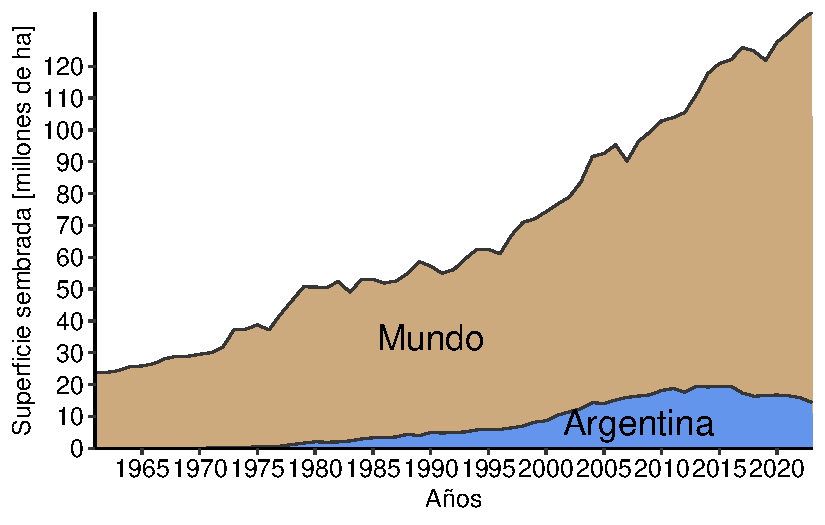
\includegraphics[width=1\textwidth,height=\textheight]{curso_R_2025_q_files/figure-pdf/unnamed-chunk-117-1.pdf}

}

\end{figure}

Entonces ahora nos queda un idea mucho mejor de cómo a crecido la
superficie sembrada de Argentina respecto a la del resto del mundo.

Aquí hemos expuesto otra de las funcionalidades que nos facilita
ggplot2: introducir más de un geom a la vez. Este puede ser del mismo
tipo o diferente, como veremos a continuación.

\hypertarget{combinando-gruxe1ficos-de-distinto-tipo}{%
\subsection{Combinando gráficos de distinto
tipo}\label{combinando-gruxe1ficos-de-distinto-tipo}}

También puede resultarnos de utilidad combinar gráficos de dos tipos
diferentes. Esta opción es muy útil y sencilla de utilizar, sin embargo
hay un par de condiciones a cumplir:

\begin{itemize}
\tightlist
\item
  el eje x debe ser el mismo.
\item
  el eje y también debe ser el mismo, o al menos ser ``compatible'' en
  escala (podría introducirse un eje secundario, pero excede al
  contenido de este taller).
\end{itemize}

Una vez cumplidas estas condiciones, es solo cuestión de usar nuestra
creatividad para crear el mejor gráfico. Supongamos como ejemplo que
queremos comparar el rendimiento de la soja en Argentina contra el
promedio mundial. Podemos hacer un gráfico de columnas clasificando por
región:

\begin{Shaded}
\begin{Highlighting}[]
\NormalTok{soja }\SpecialCharTok{\%\textgreater{}\%} \FunctionTok{mutate}\NormalTok{(}\AttributeTok{Area=}\FunctionTok{fct\_recode}\NormalTok{(Area,}
                              \StringTok{"Argentina"}\OtherTok{=}\StringTok{"Argentine"}\NormalTok{, }\CommentTok{\# modificamos los factores al español}
                              \StringTok{"Mundo"} \OtherTok{=}\StringTok{"World"}\NormalTok{)) }\SpecialCharTok{\%\textgreater{}\%}
\FunctionTok{ggplot}\NormalTok{(}\FunctionTok{aes}\NormalTok{(Year, Yield}\SpecialCharTok{/}\DecValTok{1000}\NormalTok{, }\AttributeTok{fill=}\NormalTok{Area))}\SpecialCharTok{+}
  \FunctionTok{geom\_col}\NormalTok{(}\AttributeTok{position=}\StringTok{"dodge"}\NormalTok{) }\SpecialCharTok{+}
  \FunctionTok{scale\_y\_continuous}\NormalTok{(}\AttributeTok{expand =} \FunctionTok{c}\NormalTok{(}\DecValTok{0}\NormalTok{,}\DecValTok{0}\NormalTok{), }\AttributeTok{breaks =} \FunctionTok{seq}\NormalTok{(}\DecValTok{0}\NormalTok{,}\DecValTok{5}\NormalTok{, }\AttributeTok{by =}\NormalTok{ .}\DecValTok{5}\NormalTok{))}\SpecialCharTok{+}
  \FunctionTok{scale\_x\_continuous}\NormalTok{(}\AttributeTok{expand =} \FunctionTok{c}\NormalTok{(}\DecValTok{0}\NormalTok{,}\DecValTok{0}\NormalTok{),}\AttributeTok{breaks =} \FunctionTok{seq}\NormalTok{(}\DecValTok{1960}\NormalTok{,}\DecValTok{2025}\NormalTok{, }\AttributeTok{by=}\DecValTok{5}\NormalTok{))}\SpecialCharTok{+}
  \FunctionTok{labs}\NormalTok{(}\AttributeTok{x=} \StringTok{"Años"}\NormalTok{,}
       \AttributeTok{y=} \StringTok{"Rendimiento [Tn/ha]"}\NormalTok{)}\SpecialCharTok{+}
\NormalTok{  THEME }\SpecialCharTok{+}
  \FunctionTok{theme}\NormalTok{(}\AttributeTok{legend.position =} \FunctionTok{c}\NormalTok{(.}\DecValTok{2}\NormalTok{,.}\DecValTok{85}\NormalTok{))}
\end{Highlighting}
\end{Shaded}

\begin{figure}[H]

{\centering 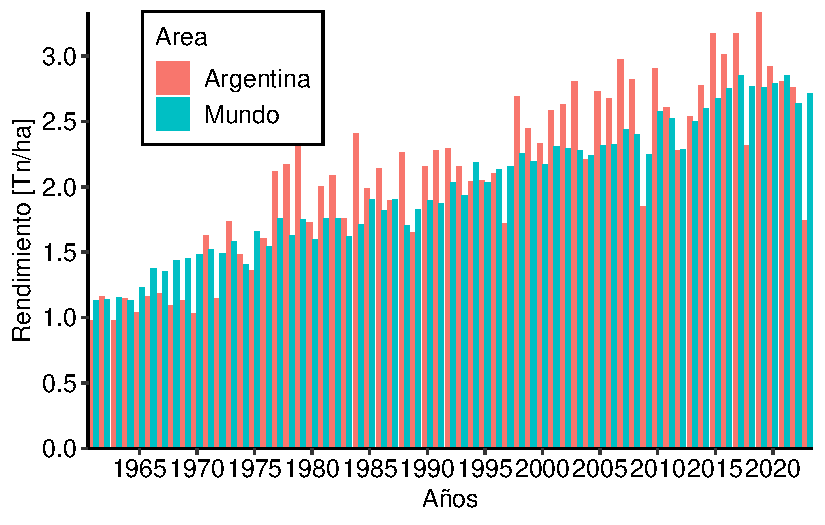
\includegraphics[width=1\textwidth,height=\textheight]{curso_R_2025_q_files/figure-pdf/unnamed-chunk-118-1.pdf}

}

\end{figure}

Como vemos, de esta manera nos quedan demasiadas columnas y es muy
difícil tener una idea clara del patrón. En cambio vamos a colocar el
rendimiento global como puntos unidos por una línea. Para ello
utilizaremos las bases de datos argentina y mundo. Además vemos que las
comas del eje Y aparecen como puntos, lo modificaremos al formato del
español:

\begin{Shaded}
\begin{Highlighting}[]
\FunctionTok{ggplot}\NormalTok{(argentina, }\FunctionTok{aes}\NormalTok{(Year, Yield}\SpecialCharTok{/}\DecValTok{1000}\NormalTok{))}\SpecialCharTok{+} \CommentTok{\# base de datos de argentina}
  \FunctionTok{geom\_col}\NormalTok{(}\AttributeTok{fill=}\StringTok{"cornflowerblue"}\NormalTok{) }\SpecialCharTok{+}  \CommentTok{\# creamos las columnas}
  \FunctionTok{scale\_y\_continuous}\NormalTok{(}\AttributeTok{expand =} \FunctionTok{c}\NormalTok{(}\DecValTok{0}\NormalTok{,}\DecValTok{0}\NormalTok{), }\AttributeTok{breaks =} \FunctionTok{seq}\NormalTok{(}\DecValTok{0}\NormalTok{,}\DecValTok{5}\NormalTok{, }\AttributeTok{by =}\NormalTok{ .}\DecValTok{5}\NormalTok{),}
                     \AttributeTok{labels=}\ControlFlowTok{function}\NormalTok{(x) }\FunctionTok{format}\NormalTok{(x, }\AttributeTok{decimal.mark =} \StringTok{","}\NormalTok{, }\CommentTok{\# cambio . por ,}
                                               \AttributeTok{scientific =} \ConstantTok{FALSE}\NormalTok{))}\SpecialCharTok{+}
  \FunctionTok{scale\_x\_continuous}\NormalTok{(}\AttributeTok{expand =} \FunctionTok{c}\NormalTok{(}\DecValTok{0}\NormalTok{,}\DecValTok{0}\NormalTok{),}\AttributeTok{breaks =} \FunctionTok{seq}\NormalTok{(}\DecValTok{1960}\NormalTok{,}\DecValTok{2025}\NormalTok{, }\AttributeTok{by=}\DecValTok{5}\NormalTok{))}\SpecialCharTok{+}
  \FunctionTok{labs}\NormalTok{(}\AttributeTok{x=} \StringTok{"Años"}\NormalTok{,}
       \AttributeTok{y=} \StringTok{"Rendimiento [Tn/ha]"}\NormalTok{)}\SpecialCharTok{+}
  \FunctionTok{geom\_line}\NormalTok{(}\AttributeTok{data=}\NormalTok{ mundo, }\FunctionTok{aes}\NormalTok{(Year, Yield}\SpecialCharTok{/}\DecValTok{1000}\NormalTok{), }\CommentTok{\# segundo geom, del mundo}
            \AttributeTok{col=}\StringTok{"red"}\NormalTok{)}\SpecialCharTok{+}
  \FunctionTok{geom\_point}\NormalTok{(}\AttributeTok{data=}\NormalTok{ mundo, }\FunctionTok{aes}\NormalTok{(Year, Yield}\SpecialCharTok{/}\DecValTok{1000}\NormalTok{), }\CommentTok{\# tercer geom, de nuevo hay que especificar}
            \AttributeTok{col=}\StringTok{"red"}\NormalTok{, }\AttributeTok{size=}\DecValTok{2}\NormalTok{)}\SpecialCharTok{+}
  \FunctionTok{annotate}\NormalTok{(}\StringTok{"text"}\NormalTok{, }\AttributeTok{x=}\DecValTok{1990}\NormalTok{, }\AttributeTok{y=} \FloatTok{2.5}\NormalTok{, }\AttributeTok{label =} \StringTok{"Argentina"}\NormalTok{, }\AttributeTok{col=}\StringTok{"cornflowerblue"}\NormalTok{, }\AttributeTok{size=}\DecValTok{5}\NormalTok{)}\SpecialCharTok{+}
  \FunctionTok{annotate}\NormalTok{(}\StringTok{"text"}\NormalTok{, }\AttributeTok{x=}\DecValTok{1965}\NormalTok{, }\AttributeTok{y=} \FloatTok{1.6}\NormalTok{, }\AttributeTok{label =} \StringTok{"Mundo"}\NormalTok{, }\AttributeTok{col=}\StringTok{"red"}\NormalTok{, }\AttributeTok{size=}\DecValTok{5}\NormalTok{) }\SpecialCharTok{+}
\NormalTok{  THEME}
\end{Highlighting}
\end{Shaded}

\begin{figure}[H]

{\centering 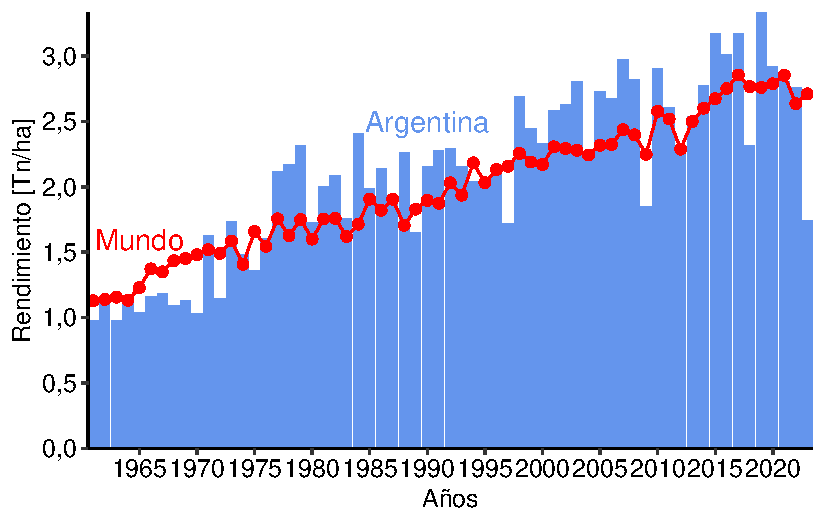
\includegraphics[width=1\textwidth,height=\textheight]{curso_R_2025_q_files/figure-pdf/unnamed-chunk-119-1.pdf}

}

\end{figure}

Ahora nos resulta mucho más fácil diferenciar en qué años (o períodos)
el rendimiento fue mayor en Argentina que el promedio global.

\hypertarget{eje-secundario}{%
\paragraph{Eje secundario}\label{eje-secundario}}

Si bien el uso de gráficos con ejes secundarios no fue planteado por el
creador de ggplot2 por no considerarlo útil (idea que comparto), se
puede incorporar mediante el parámetro \emph{sec.axis} dentro de
\emph{scale\_y\_continuos} . Es importante destacar que este eje
secundario se debe plantear como una transformación del eje primario.
Esto limita fuertemente su uso, y en este curso simplemente
aproximaremos una forma de hacerlo para ilustrar la segunda variable de
una forma ``aproximada''.

Supongamos que queremos graficar, siguiendo con nuestra base de datos,
el rendimiento y la producción de soja en Argentina a lo largo del
tiempo, en el mismo gráfico. Tomaremos como eje primario el de
rendimiento, y secundario el de producción. Como un eje tiene que se una
proporción del otro, creamos una nueva variable que nos indique la
relación entre ellos:

\begin{Shaded}
\begin{Highlighting}[]
\NormalTok{argentina }\OtherTok{\textless{}{-}}\NormalTok{ argentina }\SpecialCharTok{\%\textgreater{}\%} 
  \FunctionTok{mutate}\NormalTok{(}\AttributeTok{Relacion =}\NormalTok{ Production}\SpecialCharTok{/}\NormalTok{(Yield}\SpecialCharTok{/}\DecValTok{1000}\NormalTok{))}
\end{Highlighting}
\end{Shaded}

Y luego utilizaremos el valor máximo de estar relación para graficar y
que ambas variables se ``observen'' en una escala similar. Luego
deberemos realizar una conversión de la escala a poner en el eje
secundario siguiendo un patrón similar. Como vamos a usar la relación
máxima entre rendimiento y producción, el valor graficado será
aproximado ya que cada año dicha relación será diferente. Sin embargo,
veremos que la aproximación es bastante buena y sirve de forma
representativa.

\begin{Shaded}
\begin{Highlighting}[]
\FunctionTok{ggplot}\NormalTok{(argentina, }\FunctionTok{aes}\NormalTok{(}\AttributeTok{x=}\NormalTok{Year))}\SpecialCharTok{+} \CommentTok{\# especificamos el eje x}
  \FunctionTok{geom\_col}\NormalTok{(}\FunctionTok{aes}\NormalTok{(}\AttributeTok{y=}\NormalTok{Yield}\SpecialCharTok{/}\DecValTok{1000}\NormalTok{),  }\CommentTok{\# luego en cada geom el eje y}
           \AttributeTok{fill=}\StringTok{"darkolivegreen2"}\NormalTok{) }\SpecialCharTok{+}
  \FunctionTok{scale\_y\_continuous}\NormalTok{(}\AttributeTok{expand =} \FunctionTok{c}\NormalTok{(}\DecValTok{0}\NormalTok{,}\DecValTok{0}\NormalTok{), }\AttributeTok{limits=}\FunctionTok{c}\NormalTok{(}\DecValTok{0}\NormalTok{,}\FloatTok{3.5}\NormalTok{),}
                     \AttributeTok{breaks =} \FunctionTok{seq}\NormalTok{(}\DecValTok{0}\NormalTok{,}\DecValTok{5}\NormalTok{, }\AttributeTok{by =}\NormalTok{ .}\DecValTok{5}\NormalTok{), }
                     \AttributeTok{sec.axis =}
                       \FunctionTok{sec\_axis}\NormalTok{(}\SpecialCharTok{\textasciitilde{}}\NormalTok{.}\SpecialCharTok{*}\FunctionTok{max}\NormalTok{(argentina}\SpecialCharTok{$}\NormalTok{Relacion)}\SpecialCharTok{/}\DecValTok{1000000}\NormalTok{, }\CommentTok{\#la relación de los ejes  }
                        \AttributeTok{name=}\StringTok{"Producción [millones de Tn]"}\NormalTok{, }\CommentTok{\# título}
                        \AttributeTok{breaks=}\FunctionTok{seq}\NormalTok{(}\DecValTok{0}\NormalTok{,}\DecValTok{65}\NormalTok{, }\AttributeTok{by=}\DecValTok{5}\NormalTok{)))}\SpecialCharTok{+}
  \FunctionTok{scale\_x\_continuous}\NormalTok{(}\AttributeTok{expand =} \FunctionTok{c}\NormalTok{(}\DecValTok{0}\NormalTok{,}\DecValTok{0}\NormalTok{),}\AttributeTok{breaks =} \FunctionTok{seq}\NormalTok{(}\DecValTok{1960}\NormalTok{,}\DecValTok{2023}\NormalTok{, }\AttributeTok{by=}\DecValTok{5}\NormalTok{))}\SpecialCharTok{+}
  \FunctionTok{labs}\NormalTok{(}\AttributeTok{x=} \StringTok{"Años"}\NormalTok{,}
       \AttributeTok{y=} \StringTok{"Rendimiento [Tn/ha]"}\NormalTok{)}\SpecialCharTok{+}
  \FunctionTok{geom\_line}\NormalTok{(}\FunctionTok{aes}\NormalTok{(}\AttributeTok{y=}\NormalTok{Production}\SpecialCharTok{/}\FunctionTok{max}\NormalTok{(Relacion)), }
            \AttributeTok{col=}\StringTok{"blue3"}\NormalTok{)}\SpecialCharTok{+} 
  \FunctionTok{geom\_point}\NormalTok{(}\FunctionTok{aes}\NormalTok{(}\AttributeTok{y=}\NormalTok{Production}\SpecialCharTok{/}\FunctionTok{max}\NormalTok{(Relacion)), }
            \AttributeTok{col=}\StringTok{"blue3"}\NormalTok{, }\AttributeTok{size =} \DecValTok{4}\NormalTok{)}\SpecialCharTok{+}
  \FunctionTok{annotate}\NormalTok{(}\StringTok{"text"}\NormalTok{, }\AttributeTok{x=}\DecValTok{1990}\NormalTok{, }\AttributeTok{y=} \FloatTok{2.5}\NormalTok{, }\AttributeTok{label =} \StringTok{"Rendimiento"}\NormalTok{, }\AttributeTok{col=}\StringTok{"darkolivegreen4"}\NormalTok{, }\AttributeTok{size=}\DecValTok{6}\NormalTok{)}\SpecialCharTok{+}
  \FunctionTok{annotate}\NormalTok{(}\StringTok{"text"}\NormalTok{, }\AttributeTok{x=}\DecValTok{2010}\NormalTok{, }\AttributeTok{y=} \DecValTok{1}\NormalTok{, }\AttributeTok{label =} \StringTok{"Producción"}\NormalTok{, }\AttributeTok{col=}\StringTok{"blue3"}\NormalTok{, }\AttributeTok{size=}\DecValTok{6}\NormalTok{) }\SpecialCharTok{+}
\NormalTok{  THEME}
\end{Highlighting}
\end{Shaded}

\begin{figure}[H]

{\centering 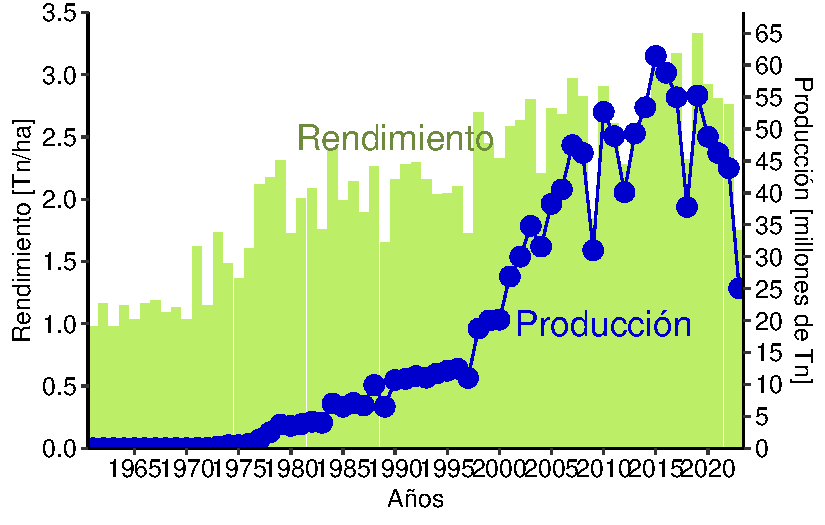
\includegraphics[width=1\textwidth,height=\textheight]{curso_R_2025_q_files/figure-pdf/unnamed-chunk-121-1.pdf}

}

\end{figure}

\hypertarget{pivoteando-pivoting}{%
\subsection{Pivoteando (pivoting)}\label{pivoteando-pivoting}}

La última funcionalidad que veremos en este taller es el uso de
\texttt{pivot\_longer} y \texttt{pivot\_wider}. Estas dos funciones
tienen usos opuestos y veremos de a una cómo se usan, ya que nos permite
transformar completamente la estructura de la base de datos, a partir de
intercambiar columnas por filas (o viceversa).

\hypertarget{pivot_longer}{%
\subsubsection{pivot\_longer}\label{pivot_longer}}

Nos permite agrupar diferentes variables (que tengamos en varias
columnas) en una que contenga el nombre de la categoría (que antes era
el nombre de una columna) y otra que contenga el valor numérico que
corresponde a cada una. Nada mejor para ilustrarlo que un ejemplo.
Recordemos nuestra base de datos \emph{soja} que tenía esta estructura
inicial:

\begin{Shaded}
\begin{Highlighting}[]
\FunctionTok{head}\NormalTok{(soja)}
\end{Highlighting}
\end{Shaded}

\begin{verbatim}
# A tibble: 6 x 6
  Area      Element         Year   Sup Production Yield
  <chr>     <chr>          <dbl> <dbl>      <dbl> <dbl>
1 Argentina Area harvested  1961   980        957   977
2 Argentina Area harvested  1962  9649      11220  1163
3 Argentina Area harvested  1963 19302      18920   980
4 Argentina Area harvested  1964 12220      14000  1146
5 Argentina Area harvested  1965 16422      17000  1035
6 Argentina Area harvested  1966 15689      18200  1160
\end{verbatim}

Supongamos ahora que queremos crear una columna que contenga en sus
filas el tipo de parámetro que estamos midiendo (superficie, producción
o rendimiento) y otra que contenga el valor del parámetro
correspondiente. La estructura básica de \texttt{pivot\_longer} es la
siguiente:

\begin{Shaded}
\begin{Highlighting}[]
\FunctionTok{pivot\_longer}\NormalTok{(}\FunctionTok{c}\NormalTok{(}\StringTok{\textasciigrave{}}\AttributeTok{variable\_1}\StringTok{\textasciigrave{}}\NormalTok{, }\StringTok{\textasciigrave{}}\AttributeTok{variable\_2}\StringTok{\textasciigrave{}}\NormalTok{, ... , }\StringTok{\textasciigrave{}}\AttributeTok{variable\_n}\StringTok{\textasciigrave{}}\NormalTok{), }\CommentTok{\# variables a combinar}
       \AttributeTok{names\_to =} \StringTok{"Variables"}\NormalTok{, }\CommentTok{\# el titulo de la nueva columna con las variables}
       \AttributeTok{values\_to =} \StringTok{"Valor"}\NormalTok{) }\CommentTok{\# el título de la nueva columna con el valor numérico}
\end{Highlighting}
\end{Shaded}

Notar que el nombre de las variables se debe introducir entre tildes
invertidas (`). En nuestro caso de ejemplo será:

\begin{Shaded}
\begin{Highlighting}[]
\NormalTok{soja }\SpecialCharTok{\%\textgreater{}\%} \FunctionTok{pivot\_longer}\NormalTok{(}\FunctionTok{c}\NormalTok{(}\StringTok{\textasciigrave{}}\AttributeTok{Sup}\StringTok{\textasciigrave{}}\NormalTok{, }\StringTok{\textasciigrave{}}\AttributeTok{Yield}\StringTok{\textasciigrave{}}\NormalTok{, }\StringTok{\textasciigrave{}}\AttributeTok{Production}\StringTok{\textasciigrave{}}\NormalTok{),}
       \AttributeTok{names\_to =}  \StringTok{"Variables"}\NormalTok{,}
       \AttributeTok{values\_to =} \StringTok{"Valor"}\NormalTok{)}
\end{Highlighting}
\end{Shaded}

\begin{verbatim}
# A tibble: 378 x 5
   Area      Element         Year Variables  Valor
   <chr>     <chr>          <dbl> <chr>      <dbl>
 1 Argentina Area harvested  1961 Sup          980
 2 Argentina Area harvested  1961 Yield        977
 3 Argentina Area harvested  1961 Production   957
 4 Argentina Area harvested  1962 Sup         9649
 5 Argentina Area harvested  1962 Yield       1163
 6 Argentina Area harvested  1962 Production 11220
 7 Argentina Area harvested  1963 Sup        19302
 8 Argentina Area harvested  1963 Yield        980
 9 Argentina Area harvested  1963 Production 18920
10 Argentina Area harvested  1964 Sup        12220
# i 368 more rows
\end{verbatim}

\hypertarget{pivot_wider}{%
\subsubsection{pivot\_wider}\label{pivot_wider}}

La función \texttt{pivot\_wider} hace exactamente lo contrario que
\texttt{pivot\_longer}, nos permite a partir de una columna con varios
niveles de un factor, crear múltiples columnas (una para cada nivel del
factor). Para utilizarla, cada fila que tengamos tiene que ser única (es
decir, lo elementos que no son variables respuestas no pueden ser los
mismos entre dos filas) para que no se genere confusión. La estructura
general es la siguiente:

\begin{Shaded}
\begin{Highlighting}[]
\FunctionTok{pivot\_wider}\NormalTok{(}\AttributeTok{names\_from =}\NormalTok{ variable, }\CommentTok{\# variable a dividir}
       \AttributeTok{values\_from =}\NormalTok{ Valor) }\CommentTok{\# variable respuesta numérica a repartir}
\end{Highlighting}
\end{Shaded}

Entonces, a modo de ejemplo, supongamos que queremos comparar como se ha
incrementado la producción de soja en Argentina y el mundo desde 1961
hasta 2023. Para ello podemos primero seleccionar las variables de
interés (solo nos interesa la producción), después filtrar los años de
interés y crear nuevas columnas.

\begin{Shaded}
\begin{Highlighting}[]
\NormalTok{soja }\SpecialCharTok{\%\textgreater{}\%} \FunctionTok{select}\NormalTok{(Area, Year, Production) }\SpecialCharTok{\%\textgreater{}\%} \CommentTok{\# seleccionamos}
  \FunctionTok{filter}\NormalTok{(Year}\SpecialCharTok{==}\DecValTok{1961} \SpecialCharTok{|}\NormalTok{ Year}\SpecialCharTok{==}\DecValTok{2023}\NormalTok{) }\SpecialCharTok{\%\textgreater{}\%}  \CommentTok{\# filtramos}
  \FunctionTok{pivot\_wider}\NormalTok{(}\AttributeTok{names\_from =}\NormalTok{  Year, }\AttributeTok{values\_from =}\NormalTok{ Production) }\SpecialCharTok{\%\textgreater{}\%} \CommentTok{\# repartimos en columnas}
  \FunctionTok{mutate}\NormalTok{(}\AttributeTok{Prop=} \FunctionTok{round}\NormalTok{(}\StringTok{\textasciigrave{}}\AttributeTok{2023}\StringTok{\textasciigrave{}}\SpecialCharTok{/}\StringTok{\textasciigrave{}}\AttributeTok{1961}\StringTok{\textasciigrave{}}\NormalTok{, }\DecValTok{0}\NormalTok{)) }\CommentTok{\# transformamos con las variables entre \textasciigrave{} \textasciigrave{}}
\end{Highlighting}
\end{Shaded}

\begin{verbatim}
# A tibble: 2 x 4
  Area        `1961`    `2023`  Prop
  <chr>        <dbl>     <dbl> <dbl>
1 Argentina      957  25044978 26170
2 World     26883158 371173609    14
\end{verbatim}

Podemos ver como en Argentina en el último medio siglo se incrementó la
producción 26170 veces, mientras que a nivel global 1381 veces.

Estas funciones tienen diferentes usos. Como vimos,
\texttt{pivot\_wider} puede servirnos para convertir variables y
comparar niveles de un factor. \texttt{pivot\_longer} puede servir tanto
para corregir bases mal armadas como para generar nuevos criterios de
clasificación que pueden ser útiles en algunos gráficos.

Por ejemplo final, supongamos que queremos ver en un mismo gráfico qué
porcentaje de la producción global y de la superficie global sembrada
representa Argentina. Para ello vamos a:

\begin{itemize}
\tightlist
\item
  seleccionar las columnas de interés
\item
  unir producción y superficie en una única columna
  (\texttt{pivot\_longer})
\item
  dividir Argentina y Mundo en dos columnas (\texttt{pivot\_wider})
\item
  calcular la proporción que representa Argentina del global y con ella
  el porcentaje
\item
  graficar aplicando como criterio de clasificación del color la columna
  que especifica si se trata de producción o superficie.
\end{itemize}

Quedaría de la siguiente manera:

\begin{Shaded}
\begin{Highlighting}[]
\NormalTok{soja }\SpecialCharTok{\%\textgreater{}\%}
  \FunctionTok{select}\NormalTok{(Area, Year, Sup, Production)}\SpecialCharTok{\%\textgreater{}\%}
  \FunctionTok{pivot\_longer}\NormalTok{(}\FunctionTok{c}\NormalTok{(}\StringTok{\textasciigrave{}}\AttributeTok{Sup}\StringTok{\textasciigrave{}}\NormalTok{, }\StringTok{\textasciigrave{}}\AttributeTok{Production}\StringTok{\textasciigrave{}}\NormalTok{), }\AttributeTok{names\_to =} \StringTok{"variable"}\NormalTok{, }\AttributeTok{values\_to =} \StringTok{"value"}\NormalTok{) }\SpecialCharTok{\%\textgreater{}\%}
  \FunctionTok{pivot\_wider}\NormalTok{(}\AttributeTok{names\_from =}\NormalTok{ Area, }\AttributeTok{values\_from =}\NormalTok{ value) }\SpecialCharTok{\%\textgreater{}\%}
  \FunctionTok{mutate}\NormalTok{(}
    \AttributeTok{prop =}\NormalTok{ Argentina}\SpecialCharTok{/}\NormalTok{World,}
    \AttributeTok{porc =}\NormalTok{ prop}\SpecialCharTok{*}\DecValTok{100}  \CommentTok{\# notar que podemos usar la variable recién creada}
\NormalTok{  )}\SpecialCharTok{\%\textgreater{}\%}
  \FunctionTok{ggplot}\NormalTok{(}\FunctionTok{aes}\NormalTok{(Year, porc, }\AttributeTok{col=}\NormalTok{variable))}\SpecialCharTok{+}
  \FunctionTok{geom\_point}\NormalTok{()}\SpecialCharTok{+}
  \FunctionTok{geom\_line}\NormalTok{()}\SpecialCharTok{+}
  \FunctionTok{scale\_y\_continuous}\NormalTok{(}\AttributeTok{limits=}\FunctionTok{c}\NormalTok{(}\DecValTok{0}\NormalTok{,}\DecValTok{30}\NormalTok{),}\AttributeTok{expand =} \FunctionTok{c}\NormalTok{(}\DecValTok{0}\NormalTok{,}\DecValTok{0}\NormalTok{), }\AttributeTok{breaks =} \FunctionTok{seq}\NormalTok{(}\DecValTok{0}\NormalTok{, }\DecValTok{25}\NormalTok{, }\AttributeTok{by =} \DecValTok{2}\NormalTok{))}\SpecialCharTok{+}
  \FunctionTok{scale\_x\_continuous}\NormalTok{(}\AttributeTok{expand =} \FunctionTok{c}\NormalTok{(}\DecValTok{0}\NormalTok{,}\DecValTok{0}\NormalTok{),}\AttributeTok{breaks =} \FunctionTok{seq}\NormalTok{(}\DecValTok{1960}\NormalTok{,}\DecValTok{2025}\NormalTok{, }\AttributeTok{by=}\DecValTok{5}\NormalTok{))}\SpecialCharTok{+}
  \FunctionTok{labs}\NormalTok{(}\AttributeTok{x=} \StringTok{"Años"}\NormalTok{,}
       \AttributeTok{y=} \StringTok{"Porcentaje del global"}\NormalTok{)}\SpecialCharTok{+}
  \FunctionTok{scale\_colour\_manual}\NormalTok{(}\AttributeTok{values=}\FunctionTok{c}\NormalTok{(}\StringTok{"Sup"}\OtherTok{=} \StringTok{"blue4"}\NormalTok{,}\StringTok{"Production"}\OtherTok{=}\StringTok{"red"}\NormalTok{), }\AttributeTok{guide=} \StringTok{"none"}\NormalTok{)}\SpecialCharTok{+}
  \FunctionTok{annotate}\NormalTok{(}\StringTok{"text"}\NormalTok{, }\AttributeTok{x=}\DecValTok{2007}\NormalTok{, }\AttributeTok{y=}\DecValTok{10}\NormalTok{, }\AttributeTok{label=}\StringTok{"Superficie}\SpecialCharTok{\textbackslash{}n}\StringTok{cultivada"}\NormalTok{, }\AttributeTok{col=}\StringTok{"blue4"}\NormalTok{, }\AttributeTok{size=}\DecValTok{5}\NormalTok{)}\SpecialCharTok{+}
  \FunctionTok{annotate}\NormalTok{(}\StringTok{"text"}\NormalTok{, }\AttributeTok{x=}\DecValTok{1995}\NormalTok{, }\AttributeTok{y=}\DecValTok{18}\NormalTok{, }\AttributeTok{label=}\StringTok{"Producción"}\NormalTok{, }\AttributeTok{col=}\StringTok{"red"}\NormalTok{, }\AttributeTok{size=}\DecValTok{5}\NormalTok{) }\SpecialCharTok{+}
\NormalTok{  THEME}
\end{Highlighting}
\end{Shaded}

\begin{figure}[H]

{\centering 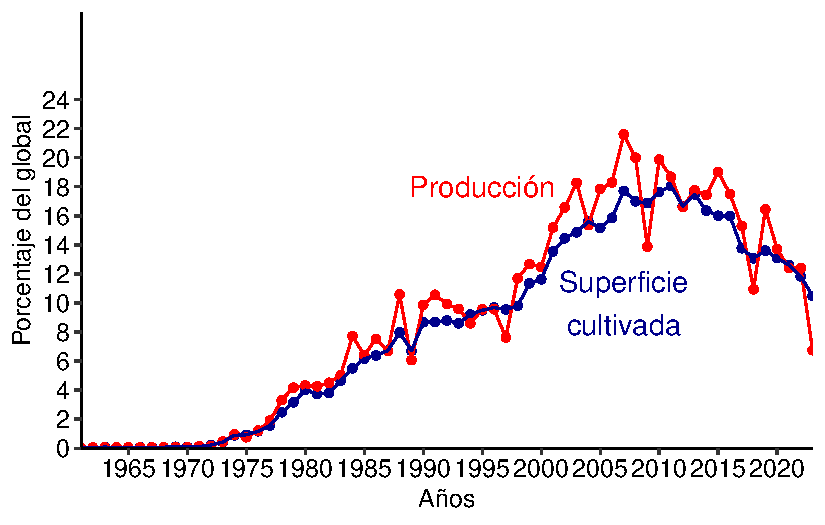
\includegraphics[width=1\textwidth,height=\textheight]{curso_R_2025_q_files/figure-pdf/unnamed-chunk-127-1.pdf}

}

\end{figure}

\hypertarget{gruxe1ficos-de-biplot-para-anuxe1lisis-multivariado}{%
\subsection{Gráficos de biplot para análisis
multivariado}\label{gruxe1ficos-de-biplot-para-anuxe1lisis-multivariado}}

Esta sección tiene por objetivo mostrar que el conocimiento de los
gráficos con ggplot2 sobrepasan al uso individual de este paquete, sino
que hay mucho otros que se basan en él para generar gráficos. Un ejemplo
de ello es el paquete \emph{factoextra} para gráficos multivariados.

Vamos a desarrollar un ejemplo donde armamos un biplot a partir de un
análisis de componentes principales (PCA). Vamos a retomar a la base de
datos ALIM, y haremos un PCA comparando la concentración de distintos
metales en los órganos, su peso seco y verdor. Para ello ejecutamos:

\begin{Shaded}
\begin{Highlighting}[]
\FunctionTok{library}\NormalTok{(factoextra);}\FunctionTok{library}\NormalTok{(FactoMineR);}\FunctionTok{library}\NormalTok{(ggrepel)}
\end{Highlighting}
\end{Shaded}

\begin{verbatim}
Warning: package 'factoextra' was built under R version 4.4.2
\end{verbatim}

\begin{verbatim}
Welcome! Want to learn more? See two factoextra-related books at https://goo.gl/ve3WBa
\end{verbatim}

\begin{verbatim}

Adjuntando el paquete: 'factoextra'
\end{verbatim}

\begin{verbatim}
The following object is masked from 'package:agricolae':

    hcut
\end{verbatim}

\begin{verbatim}
Warning: package 'FactoMineR' was built under R version 4.4.2
\end{verbatim}

\begin{Shaded}
\begin{Highlighting}[]
\NormalTok{res.pca }\OtherTok{\textless{}{-}} \FunctionTok{PCA}\NormalTok{(ALIM[, }\SpecialCharTok{{-}}\FunctionTok{c}\NormalTok{(}\DecValTok{1}\SpecialCharTok{:}\DecValTok{5}\NormalTok{)], }\AttributeTok{scale.unit =} \ConstantTok{TRUE}\NormalTok{)}
\end{Highlighting}
\end{Shaded}

\begin{figure}[H]

{\centering 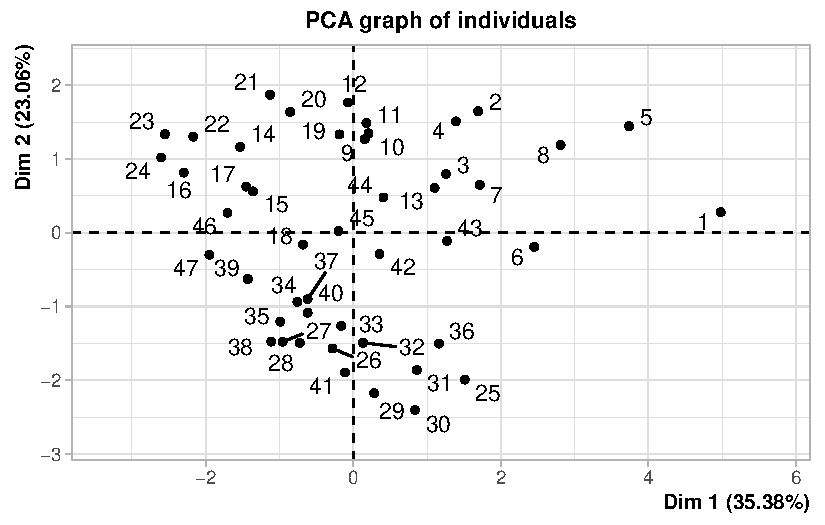
\includegraphics{curso_R_2025_q_files/figure-pdf/unnamed-chunk-128-1.pdf}

}

\end{figure}

\begin{figure}[H]

{\centering 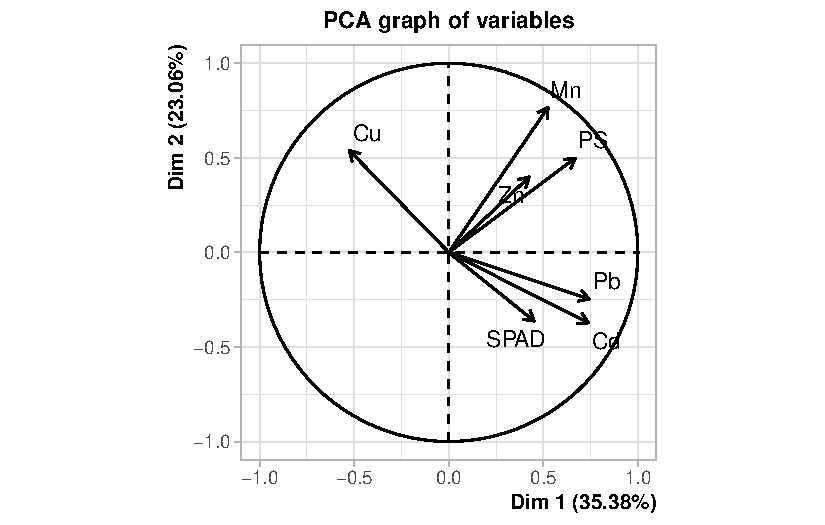
\includegraphics{curso_R_2025_q_files/figure-pdf/unnamed-chunk-128-2.pdf}

}

\end{figure}

Una vez creado el objeto de resultado de nuestro PCA, vamos a realizar
un gráfico de biplot con la función \textbf{fviz\_pca\_biplot} de
\emph{factoextra}:

\begin{Shaded}
\begin{Highlighting}[]
\NormalTok{BIPLOT }\OtherTok{\textless{}{-}} \FunctionTok{fviz\_pca\_biplot}\NormalTok{(res.pca, }
                \AttributeTok{repel =} \ConstantTok{TRUE}\NormalTok{,}
                \AttributeTok{geom.ind =} \StringTok{"point"}\NormalTok{,}
                \AttributeTok{col.var =} \StringTok{"deeppink4"}\NormalTok{, }
                \AttributeTok{col.ind =} \StringTok{"black"}\NormalTok{,}
                \AttributeTok{labelsize=}\DecValTok{5}\NormalTok{,}
                \AttributeTok{axes.linetype =} \StringTok{"blank"}\NormalTok{,}
                \AttributeTok{alpha.var=}\FloatTok{0.5}\NormalTok{,}
                \AttributeTok{title =} \ConstantTok{NULL}\NormalTok{) ; BIPLOT}
\end{Highlighting}
\end{Shaded}

\begin{figure}[H]

{\centering 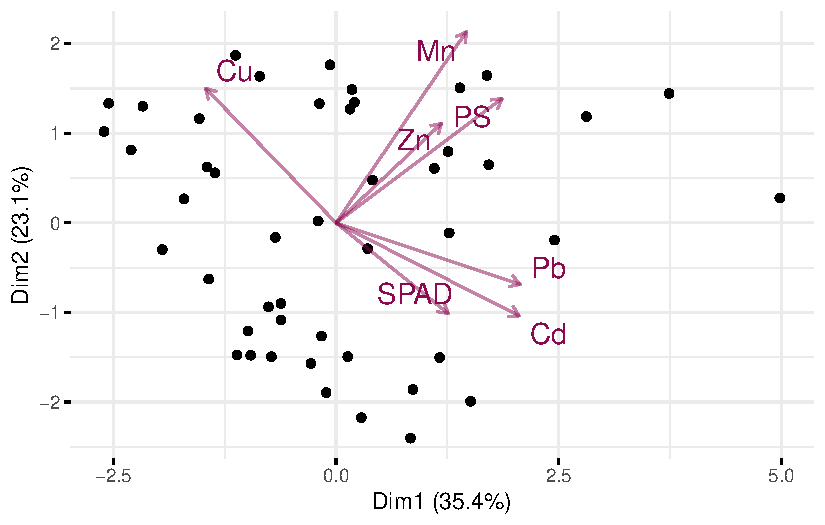
\includegraphics[width=1\textwidth,height=\textheight]{curso_R_2025_q_files/figure-pdf/unnamed-chunk-129-1.pdf}

}

\end{figure}

Ahora vamos a realizar algunas modificaciones estéticas, y a incluir una
clasificación por color según el órgano de el que se trate. Para ello
vamos a crear un objeto nuevo con los porcentajes de explicación de cada
eje:

\begin{Shaded}
\begin{Highlighting}[]
\NormalTok{VARIANCE }\OtherTok{\textless{}{-}} \FunctionTok{round}\NormalTok{(}\FunctionTok{get\_eigenvalue}\NormalTok{(res.pca)[,}\DecValTok{2}\NormalTok{], }\DecValTok{2}\NormalTok{)}


\NormalTok{BIPLOT }\SpecialCharTok{+}
  \FunctionTok{geom\_point}\NormalTok{(}\FunctionTok{aes}\NormalTok{(}\AttributeTok{col =}\NormalTok{ ALIM}\SpecialCharTok{$}\NormalTok{Organo),}\AttributeTok{size =} \DecValTok{4}\NormalTok{)}\SpecialCharTok{+}
  \FunctionTok{geom\_hline}\NormalTok{(}\AttributeTok{yintercept =} \DecValTok{0}\NormalTok{, }\AttributeTok{linetype =} \StringTok{"dotted"}\NormalTok{, }\AttributeTok{col =} \StringTok{"grey30"}\NormalTok{)}\SpecialCharTok{+}
  \FunctionTok{geom\_vline}\NormalTok{(}\AttributeTok{xintercept =} \DecValTok{0}\NormalTok{, }\AttributeTok{linetype =} \StringTok{"dotted"}\NormalTok{, }\AttributeTok{col =} \StringTok{"grey30"}\NormalTok{)}\SpecialCharTok{+}
  \FunctionTok{labs}\NormalTok{(}\AttributeTok{x =} \FunctionTok{paste}\NormalTok{(}\StringTok{"PC 1 ("}\NormalTok{, VARIANCE[[}\DecValTok{1}\NormalTok{]], }\StringTok{"\%)"}\NormalTok{),}
       \AttributeTok{y =} \FunctionTok{paste}\NormalTok{(}\StringTok{"PC 2 ("}\NormalTok{, VARIANCE[[}\DecValTok{2}\NormalTok{]], }\StringTok{"\%)"}\NormalTok{),}
       \AttributeTok{col =} \StringTok{"Órgano"}\NormalTok{) }\SpecialCharTok{+}
  \FunctionTok{scale\_y\_continuous}\NormalTok{(}\AttributeTok{expand =} \FunctionTok{c}\NormalTok{(}\DecValTok{0}\NormalTok{,}\DecValTok{0}\NormalTok{), }\AttributeTok{limits =} \FunctionTok{c}\NormalTok{(}\SpecialCharTok{{-}}\DecValTok{3}\NormalTok{,}\DecValTok{3}\NormalTok{), }
                     \AttributeTok{breaks =} \FunctionTok{seq}\NormalTok{(}\SpecialCharTok{{-}}\DecValTok{40}\NormalTok{,}\DecValTok{40}\NormalTok{, }\AttributeTok{by =} \DecValTok{1}\NormalTok{))}\SpecialCharTok{+}
  \FunctionTok{scale\_x\_continuous}\NormalTok{(}\AttributeTok{expand =} \FunctionTok{c}\NormalTok{(}\DecValTok{0}\NormalTok{,}\DecValTok{0}\NormalTok{), }\AttributeTok{limits =} \FunctionTok{c}\NormalTok{(}\SpecialCharTok{{-}}\FloatTok{5.5}\NormalTok{,}\FloatTok{5.5}\NormalTok{), }
                     \AttributeTok{breaks =} \FunctionTok{seq}\NormalTok{(}\SpecialCharTok{{-}}\DecValTok{9}\NormalTok{,}\DecValTok{9}\NormalTok{, }\AttributeTok{by =} \DecValTok{2}\NormalTok{)) }\SpecialCharTok{+}
  \FunctionTok{scale\_colour\_viridis\_d}\NormalTok{() }\SpecialCharTok{+}
\NormalTok{  THEME}
\end{Highlighting}
\end{Shaded}

\begin{figure}[H]

{\centering 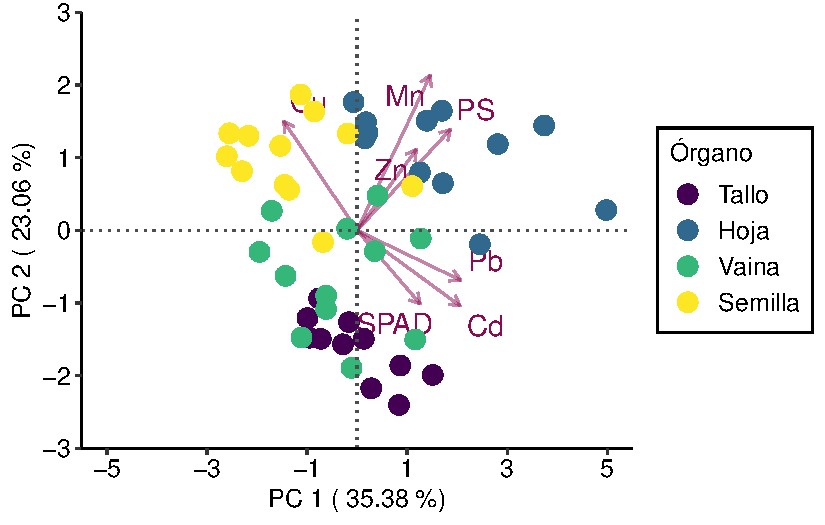
\includegraphics[width=1\textwidth,height=\textheight]{curso_R_2025_q_files/figure-pdf/unnamed-chunk-130-1.pdf}

}

\end{figure}

\href{../}{Volver al inicio}



\end{document}
